%% LyX 2.3.1-1 created this file.  For more info, see http://www.lyx.org/.
%% Do not edit unless you really know what you are doing.
\documentclass[12pt,english]{article}
\usepackage[T1]{fontenc}
\usepackage{url}
\usepackage{amsmath}
\usepackage{amsthm}
\usepackage{amssymb}
\usepackage{graphicx}
\usepackage{setspace}
\usepackage[authoryear]{natbib}
\onehalfspacing

\makeatletter

%%%%%%%%%%%%%%%%%%%%%%%%%%%%%% LyX specific LaTeX commands.
\newcommand{\noun}[1]{\textsc{#1}}
%% Because html converters don't know tabularnewline
\providecommand{\tabularnewline}{\\}

%%%%%%%%%%%%%%%%%%%%%%%%%%%%%% Textclass specific LaTeX commands.
\theoremstyle{definition}
\newtheorem{defn}{\protect\definitionname}
\theoremstyle{plain}
\newtheorem{lem}{\protect\lemmaname}
\theoremstyle{plain}
\newtheorem{prop}{\protect\propositionname}

%%%%%%%%%%%%%%%%%%%%%%%%%%%%%% User specified LaTeX commands.
%\usepackage[english]{babel}
\usepackage[scaled=.90]{helvet}
%\usepackage{mathptmx,courier}
\usepackage[a4paper, top=1.25in, left=1.25in, right=1.25in, bottom=1.25in]{geometry}
\usepackage[hidelinks]{hyperref}
\hypersetup{colorlinks=true, citecolor=BrickRed, urlcolor=BrickRed}
\usepackage{natbib}

\usepackage{array}
\usepackage[T1]{fontenc}
\usepackage{txfonts}
\usepackage{mathpazo}
\usepackage[usenames,dvipsnames]{xcolor}
%\usepackage[svgnames]{xcolor}

%\usepackage[bottom]{footmisc}
%\interfootnotelinepenalty=2147483647

\usepackage{enumerate}
\usepackage[font={large,it}]{caption}
\renewcommand{\theenumi}{\roman{enumi}}
\usepackage{graphicx}
\usepackage[export]{adjustbox}
\DeclareGraphicsExtensions{.pdf,.jpeg,.png,.eps}
\usepackage{enumitem}
\usepackage{changepage}
\strictpagecheck
\usepackage{caption}
\captionsetup{labelfont=bf,format=plain,indention=0cm,
justification=centering,singlelinecheck=false, skip=1pt}

\usepackage{booktabs}
\newcommand{\specialcell}[2][c]{%
  \begin{tabular}[#1]{@{}c@{}}#2\end{tabular}}

\author{
  Ahmad Lashkaripour \\ Indiana University
  }
\date{First Draft: May 2019 \\ This Draft: November 2020}

\usepackage{tikz}

\makeatletter
\sloppy
\makeatother
\newcounter{parentnumber}
\usepackage{multirow}
\allowdisplaybreaks
\usepackage{bbm}
\usepackage{geometry}

\makeatother

\usepackage{babel}
\providecommand{\definitionname}{Definition}
\providecommand{\lemmaname}{Lemma}
\providecommand{\propositionname}{Proposition}

\begin{document}
\title{The Cost of a Global Tariff War:\\ \emph{A Sufficient Statistics
Approach}}
\maketitle
\begin{abstract}
Tariff wars have reemerged as a serious threat to the global economy.
Yet measuring the \emph{prospective} cost of a global tariff war remains
computationally prohibitive, unless we restrict attention to a small
set of countries and industries. This paper develops a new methodology
that measures the cost of a global tariff war in one simple step as
a function of observable shares, industry-level trade elasticities,
and markup wedges. Applying this methodology to data on 44 countries
and 56 industries, I find that $(i$) the prospective cost of a global
tariff war has more-than-doubled over the past fifteen years, with
small downstream economies being the most vulnerable. $(ii)$ Meanwhile,
due to the rise of global markup distortions, the potential gains
from \emph{cooperative} tariff policies have also elevated to unprecedented
levels. 
\end{abstract}

\section{Introduction}

The global economy is entering a new era of tariffs, with many economic
leaders warning against the eminent threat of a global tariff war.
Just recently, Christine Lagarde, head of the International Monetary
Fund, labeled the escalating US-China tariff war as ``the biggest
risk to global economic growth.''\footnote{Source: \hspace{-0.65in}\url{https://www.bloomberg.com/news/articles/2019-06-09/lagarde-says-u-s-china-trade-war-looms-large-over-global-growth}} 

Concurrent with these real-world developments, there has been a growing
academic interest in measuring the cost of tariff wars. One natural
approach is the ``ex-post'' approach adopted by \citet{amiti2019impact}
and \citet{fajgelbaum2019return}. This approach, uses data on observed
tariff hikes; employs economic theory to estimate the passthrough
of tariffs onto consumer prices; and measures the welfare cost of
these \emph{already-applied} tariffs.

The evidence put forward by the ``ex-post'' approach is revealing,
but it does not speak to an outstanding policy question: \emph{what
is the prospective cost of a full-fledged global tariff war?} To answer
such ``what if'' questions, we first need to determine the non-cooperative
Nash tariff levels that will prevail under a global tariff war. The
``ex-ante'' approach undertaken by \citet{perroni2000new} and \citet{ossa2014trade}
accomplishes this exact task.\footnote{See \citet{balistreri201721st} for a recent application of the ex-ante
approach to the current US-China tariff war.} They use economic theory to estimate the Nash tariff levels that
will prevail and the welfare cost that will result from a hypothetical
(but now imminent) global tariff war. 

The ``ex-ante'' approach has been quite influential and recent methodological
advances by \citet{ossa2014trade} have made it more accessible to
researchers. Yet existing techniques are plagued with the curse of
dimensionality when applied to many countries and industries. The
current state-of-the-art technique computes the Nash tariffs using
an iterative process where each iteration performs a country-by-country
numerical optimization based on the output of the previous iterations.\footnote{See \citet{ossa2016quantitative} for a comprehensive review of the
iterative global optimization technique. Advances that have made this
technique more efficient include $(i)$ reformulating the problem
using the exact hat-algebra technique; $(ii)$ parallelizing the country-by-country
optimizations; and $(iii)$ providing analytical derivatives for the
optimization algorithm. } As the number of countries or industries grows, the computational
burden underlying this approach can raise exponentially. This is perhaps
why the current implementations of the ``ex-ante'' approach are
limited to a small set of countries and abstract from salient but
complex features of the global economy like input trade.

In this paper, I develop a simple sufficient statistics methodology
to measure the prospective cost of a global tariff war.\footnote{The sufficient statistics methodology developed here is akin to the
\citet{arkolakis2012new} methodology, and exhibits key differences
with the sufficient statistics approach popularized by \citet{chetty2009sufficient}
in the public finance literature. See Chapter 7 in \citet{costinot2014trade}
for more discussion on these differences.} My optimization-free methodology circumvents some of the main computational
challenges facing existing ``ex-ante'' techniques. This feature
allows me to uncovers the cost of a global tariff war across many
years and countries, including a long list of previously-neglected
small, emerging economies. I find that the cost of a global tariff
war has risen dramatically over the past two decades, with small downstream
economies being --by far-- the most vulnerable.

The new methodology relies on the analytical characterization of Nash
tariffs in a state-of-the-art quantitative trade model featuring multiple
industries, markup distortions, intermediate input trade, and political
economy pressures. Nash tariffs correspond to tariff levels that will
prevail in the event of a global tariff war. Prior characterizations
of Nash tariffs are impractical for my analysis, as they are limited
to \emph{partial equilibrium} or \emph{single industry-two country}
models.\footnote{See e.g., \citet{johnson1953optimum}, \citet{gros1987note}, and
\citet{felbermayr2013optimal} for a prior characterization of Nash
tariffs in two-country and single industry setups.} I, therefore, derive new analytic formulas for Nash tariffs that
are compatible with my general equilibrium, multi-country and multi-industry
analysis.\footnote{My characterization of Nash tariffs shares similarities with \citet{beshkar2017interdependence}
and \citet{lashkaripour2018scale}. The aforementioned studies analyze
\emph{unilaterally} optimal trade taxes in two-country general equilibrium
trade models. This paper analyzes many non-cooperative countries that
strategically impose tariffs against each other.} These formulas are especially advantageous as they describe Nash
tariffs as a function of observable shares and structural parameters.

Using my analytic tariff formulas and the exact hat-algebra methodology,
popularized by \citet{Dekle2007}, I can compute the Nash tariffs
and their welfare effects in one simple (optimization-free) step.
Moreover, this entire procedure can be performed with information
on only \emph{$(i)$ observable shares,} \emph{$(ii)$ industry-level}
\emph{trade elasticities}, and $(iii)$ \emph{constant industry-level
markup} \emph{wedges}. The same logic can be employed to compute the
gains from cooperative tariffs.\footnote{Specifically, I first derive an analytic formula for cooperative tariffs.
I then calibrate these formulas to data using the exact hat-algebra
technique. This procedure can be carried with knowledge of only observable
shares, trade elasticities, and markup wedges.} These are internationally coordinated tariffs that correct global
markup distortions, and are notoriously difficult to compute (\citet{ossa2016quantitative}).

The new methodology is remarkably fast: It computes the cost of a
global tariff war and the gains from future trade talks in a matter
of seconds. In comparison, optimization-based techniques may take
hours or even days, depending on the number of countries and industries
being analyzed. This improvement in speed is partly due to bypassing
the need for iterative numerical optimization. But it is also due
to a reduction in dimensionality, since analytic formulas indicate
that Nash tariffs are uniform along certain dimensions.

I apply the new methodology to the World Input-Output Database (WIOD,
\citet{timmer2012world}) from 2000 to 2014, covering 43 major countries
and 56 industries. For each country in the sample, I compute the prospective
cost of a global tariff war in each year during the 2000-2014 period.
I first perform my analysis using a baseline multi-industry \citet{Eaton2002}
model. I subsequently introduce markup distortions, political pressures,
and input trade into the baseline model to determine how these additional
factors contribute to the cost of a tariff war. May analysis delivers
four basic insights:
\begin{enumerate}
\item A global tariff war can shrink the average country's real GDP by 2.8\%.
This figure is aggravated by the increased dependence of countries
on intermediate input trade and the exacerbation of pre-existing markup
distortions. To give some perspective, the expected cost of a global
tariff war was \$1.7 trillion in 2014, when added up across all countries.
Such a cost is the equivalent of erasing South Korea from the global
economy. 
\item The prospective cost of a global tariff war has more-than-doubled
from 2000 to 2014. The rising cost is driven by two distinct forces.
First, the rise of global markup distortions, which prompts countries
to impose more-targeted (i.e., more-distortionary) Nash tariffs in
the event of a tariff war. Second, the increasing dependence of emerging
economies on intermediate input trade since 2000. 
\item Small downstream economies are the main casualties of a global tariff
war. Take Estonia, for example, where imported inputs account for
30\% of the national output inclusive of services. Due to its strong
dependence on imported inputs, 10\% of Estonia's real GDP will be
wiped out by a global tariff war. Similar losses will be incurred
by other small, downstream economies like Bulgaria, Latvia, and Luxembourg.
\item Due to the global rise of markup distortions, the gains from cooperative
tariffs have also multiplied from 2000 to 2014. Stated otherwise,
the unexplored gains from deeper trade negotiations have risen on
par with the prospective cost of a global trade war. To present some
numbers, cooperative tariffs could have added up to \$347 billion
to global GDP in 2014, up from a mere \$184 billion in 2000.
\end{enumerate}
Aside from the already-discussed methodological contribution, this
paper makes three conceptual contributions to the literature. First,
my analytic formulas for Nash tariffs highlight a previously overlooked
contributor to the cost of tariff wars. I show that Nash tariffs (in
all countries) are targeted at high-markup industries. As a result,
they shrink global output in high-markup industries below their already
sub-optimal level. These developments exacerbate pre-existing market
distortions and inflict an efficiency loss that is distinct from the
standard trade-loss emphasized in the prior literature (e.g., \citet{gros1987note}).

Second, this paper sheds new light on the winners and losers of global
tariff wars. Since \citet{johnson1953optimum}, an immense body of
literature has emphasized that country size dictates the winners (\citet{kennan2013big}).
My analysis shows that a country's dependence on imported input is
an equally-determining factor. For instance, Norway that is a net
exporter in upstream industries (due its commodity exports) can gain
from a global tariff war despite being small. These gains obviously
come at the expense of small downstream economies incurring significant
losses. These findings, though, assume that governments apply tariffs-subject-to-duty-drawbacks,
which are input-output blind by design. \citet{beshkar2020cost} look
beyond this simple case and present a more comprehensive view of how
global value chains amplify the cost of a global trade war.

Third, my approach highlights the pitfalls of data aggregation, which
is common-place in the tariff war literature. To elaborate, existing
analyses of tariff wars often restrict attention to a small set of
countries and aggregate the ``rest of the world'' into one taxing
authority. Such aggregation schemes allow researchers to handle the
computational complexities inherent to tariff war analysis. Capitalizing
on the computational efficiency of my sufficient statistics approach,
I can measure the cost of a tariff war \emph{with} and \emph{without}
such aggregation schemes. Comparing the outcomes indicates that standard
aggregation schemes overstate the loss from a tariff war quite considerably.
Simply, because they artificially assign significant market power
to ``the rest of the world.''\emph{ }

Finally, at a broader level, the approach developed here can be viewed
as a sufficient statistics methodology to quantify \emph{the gains
from trade agreements}. In that regard, it contributes to \citet{arkolakis2012new},
\citet{costinot2014trade}, and \citet{arkolakis2015elusive} who
propose sufficient statistics methodologies that quantify the gains
from trade relative to autarky in an important class of trade models.
Like the aforementioned studies, my proposed methodology quantifies
the gains from trade, but it does so relative to a world without trade
agreements as opposed to autarky. 

This paper is organized as follows. Section 2 presents the theoretical
model, based on which a sufficient statistics approach is developed
to measure the cost of a global tariff war in Section 3. Section 4
extends the methodology to compute cooperative tariffs. Section 5
presents a quantitative implementation of the methodology. Section
6 concludes.

\section{\label{sec:Theoretical-Framework}Theoretical Framework}

The present methodology applies to a wide range of quantitative trade
models. In the interest of exposition, I begin my analysis with a
\emph{baseline} multi-industry, multi-country Ricardian model that
nests the \citet{Eaton2002} and Armington models as a special case.
I subsequently extend the baseline model to account for $(a)$ political
economy pressures and profit-shifting effects \`a la \citet{ossa2014trade},
and $(b)$ intermediate input trade under duty drawbacks. 

Throughout my analysis, I consider a global economy consisting of
$i=1,...,N$ countries and $k=1,..,K$ industries, with $\mathbb{C}$
and $\mathbb{K}$ respectively denoting the set of countries and industries.
Labor is the only \emph{primary} factor of production. Each country
$i$ is populated with $\bar{L}_{i}$ workers, each of whom supplies
one unit of labor inelastically. Workers are perfectly mobile across
industries but immobile across countries. 

\subsection{Demand}

In the baseline Ricardian model, all varieties in industry $k$ are
differentiated by country of origin, with the triplet $ji,k$ denoting
a variety corresponding to origin $j$--destination $i$--industry
$k$. Under the \citet{Eaton2002} interpretation of the model, national
product differentiation of this kind can be attributed to Ricardian
specialization within industries. The representative consumer in Country
$i$ maximizes a general utility function, which yields an indirect
utility function as follows
\begin{align}
V_{i}(Y_{i},\tilde{\textbf{P}}_{i}) & =\max_{\textbf{Q}_{i}}\ \ U(\textbf{Q}_{i})\ \ \ \ \ s.t.\ \ \tilde{\textbf{P}}_{i}\cdot\textbf{Q}_{i}=Y_{i}.\label{eq: Consumer Problem}
\end{align}
In the above problem, $Y_{i}$ denotes total income; $\textbf{Q}_{i}=\{Q_{ji,k}\}$
denotes the vector of composite consumption quantities, $\tilde{\textbf{P}}_{i}=\{\tilde{P}_{ji,k}\}$
denotes the corresponding vector of \emph{``consumer''} price indexes,
and ``$\cdot$'' is the inner product operator (i.e., $\textbf{a}\cdot\textbf{b}=\sum_{i}a_{i}b_{i}$).
To avoid any confusion, I emphasize that \emph{tilde} on the price
variable is used to distinguish between (after-tax) \emph{consumer}
and (pre-tax) \emph{producer} prices. The representative consumer's
problem yields a Marshallian demand function,
\begin{equation}
Q_{ji,k}=\mathcal{Q}_{ji,k}\left(Y_{i},\tilde{\textbf{P}}_{i}\right),\label{eq: Demand}
\end{equation}
which describes optimal consumption in country $i$ as function of
income, $Y_{i}$, and consumer prices, $\tilde{\textbf{P}}_{i}$.
When analyzing optimal tariff policy in each country, several demand-side
variables play a key role. First, expenditure shares which represent
the importance of each good in the consumption basket. Second, demand
elasticities, which summarize the demand function specified under
Equation \ref{eq: Demand}. Below, I formally define these set of
variables. 
\begin{defn}
{[}\textbf{Expenditure Shares}{]}\emph{ The share of country $i$'s
expenditure on industry $k$ goods is denoted by $e_{i,k}$, and the
within-industry share of expenditure on variety $ji,k$ (origin $j$--destination
$i$--industry $k$) is denoted by $\lambda_{ji,k}$}:
\begin{align*}
e_{i,k}\equiv\frac{\tilde{\textbf{P}}_{i,k}\cdot\textbf{Q}_{i,k}}{\tilde{\textbf{P}}_{i}\cdot\textbf{Q}_{i}}=\frac{\sum_{j=1}^{N}\tilde{P}_{ji,k}Q_{ji,k}}{Y_{i}};\ \ \ \ \ \ \ \ \ \ \ \ \ \ \ \ \lambda_{ji,k}\equiv & \frac{\tilde{P}_{ji,k}Q_{ji,k}}{\tilde{\textbf{P}}_{i,k}\cdot\textbf{Q}_{i,k}}=\frac{\tilde{P}_{ji,k}Q_{ji,k}}{e_{i,k}Y_{i}}.
\end{align*}
\emph{Building on the above definitions, the unconditional expenditure
share on variety $ji,k$ ($e_{ji,k}$) and the overall share of expenditure
on goods from origin $j$ ($\lambda_{ji}$) is defined as}\vspace{-0.1in}
\[
e_{ji,k}\equiv\lambda_{ji,k}e_{i,k};\ \ \ \ \ \ \ \ \ \ \ \ \ \ \ \ \ \ \ \ \ \ \ \ \lambda_{ji}\equiv\sum_{k=1}^{K}\lambda_{ji,k}e_{i,k}.
\]
\end{defn}
Note the distinction between $e_{ji,k}$, and $\lambda_{ji,k}$. The
former concerns the share of variety $ji,k$ in total expenditure.
The latter concerns the share of expenditure on variety $ji,k$ conditional
on buying industry $k$ goods. As we will shortly, $\lambda_{ji,k}$
governs the Marshallian demand elasticities under CES preferences.
These elasticities are defined as follows for the general (not-necessarily
CES) case.
\begin{defn}
{[}\textbf{Demand Elasticities}{]} \emph{The elasticity of demand
for good $ji,k$ with respect to the price of good $ni,g$ is denoted
by}
\begin{equation}
\varepsilon_{ji,k}^{(ni,g)}\equiv\partial\ln\mathcal{Q}_{ji,k}(Y_{i},\tilde{\textbf{P}}_{i})/\partial\ln\tilde{P}_{ni,g}.\label{eq: Demand Elasticity}
\end{equation}
\emph{Correspondingly, the matrix of ``nominal'' and ``expenditure-adjusted''
demand elasticities are denoted by}
\[
\textbf{E}_{ji}^{(ni)}\equiv\left[\begin{array}{ccc}
\varepsilon_{ji,1}^{(ni,1)} & ... & \varepsilon_{ji,1}^{(ni,K)}\\
\vdots & \ddots & \vdots\\
\varepsilon_{ji,K}^{(ni,1)} & \cdots & \varepsilon_{ji,K}^{(ni,K)}
\end{array}\right];\ \ \ \ \ \ \ \ \textbf{\ensuremath{\tilde{\textbf{E}}}}_{ji}^{(ni)}\equiv\left[\begin{array}{ccc}
e_{ji,1}\varepsilon_{ji,1}^{(ni,1)} & ... & e_{ji,1}\varepsilon_{ji,1}^{(ni,K)}\\
\vdots & \ddots & \vdots\\
e_{ji,K}\varepsilon_{ji,K}^{(ni,1)} & \cdots & e_{ji,K}\varepsilon_{ji,K}^{(ni,K)}
\end{array}\right],
\]
\emph{with $\textbf{E}_{ji}\sim\textbf{E}_{ji}^{(ji)}$ denoting the
matrix of own-price elasticities of demand.}
\end{defn}
I assume that consumer preferences are well-behaved in that $\varepsilon_{ji,k}^{(ji,k)}<-1$.\footnote{The income elasticity of demand plays a less prominent role in my
analysis, so I relegate its definition to the appendix.} We can appeal to two properties of the Marshallian demand function,
namely, $(i)$ Cournot aggregation, and $(ii)$ homogeneity of degree
zero, to prove that the elasticity matrixes, $\textbf{E}_{ji}$, and
$\tilde{\textbf{E}}_{ji}$ are invertible.
\begin{lem}
The matrixes $\textbf{E}_{ji}\sim\textbf{E}_{ji}^{(ji)}$ and $\textbf{\ensuremath{\tilde{\textbf{E}}}}_{ji}\sim\textbf{\ensuremath{\tilde{\textbf{E}}}}_{ji}^{(ji)}$
are non-singular.
\end{lem}
The above lemma is formally proven in Appendix \ref{subsec: Proof Proposition-1}.
As we will see shortly, the ability to invert the elasticity matrixes
is essential for deriving sufficient statistics formulas for optimal
tariffs in each country. 

\subsection{Production}

In the baseline Ricardian model, labor is the sole factor of production
and the unit labor cost of production and transportation is invariant
to policy. Correspondingly, the ``producer'' price of composite
variety $ji,k$ can be expressed as a function of the labor wage rate
in country $j$, $w_{j}$, multiplied by the constant unit labor cost
of production, $\bar{a}_{j,k}$, and the iceberg trade cost, $\bar{\tau}_{ji,k}$
(with $\bar{\tau}_{ii,k}=1$):
\begin{equation}
P_{ji,k}=\bar{\tau}_{ji,k}\bar{a}_{j,k}w_{j}.\label{eq: Price}
\end{equation}
The \emph{bar} notation indicates that $\bar{a}_{j,k}$ and $\bar{\tau}_{ji,k}$
are invariant to policy. The ``consumer'' price, by definition,
equals the ``producer'' price times the tariff applied by country
$i$ on variety $ji,k$, namely, $t_{ji,k}$:
\begin{equation}
\tilde{P}_{ji,k}=(1+t_{ji,k})P_{ji,k}.\label{eq: Consumer Price}
\end{equation}
The invariance of $\bar{a}_{j,k}$ to policy change derives from constant
returns to scale technologies. It amounts to a flat \emph{export supply}
curve, which entails that the passthrough of taxes on to consumer
prices is complete \emph{after} we net out general equilibrium wage
effects. This assumption is consistent with ex-post studies of the
recent US-China tariff war, like \citet{amiti2019impact} and \citet{fajgelbaum2019return}.

\subsection{General Equilibrium}

Given the vector of tariffs in each country $i$, $\textbf{t}_{i}=\{t_{ji,k}\}$,
equilibrium consists of a vector of wages, $\textbf{w}=\{w_{j}\}$,
a vector of ``producer'' and ``consumer'' price indexes, $\textbf{P}_{i}=\{P_{ji,k}\}$
and $\tilde{\textbf{P}}_{i}=\{\tilde{P}_{ji,k}\}$ (as described by
Equations \ref{eq: Price} and \ref{eq: Consumer Price}), and consumption
quantities, $\textbf{Q}_{i}$, given by the Marshallian demand function
\ref{eq: Demand}, such that wage income in each country equals sales
net of taxes,\footnote{The above equation along with the representative consumer's budget
constraint, ensure that trade is balanced between countries} 
\begin{equation}
w_{i}\bar{L}_{i}=\sum_{j=1}^{N}\sum_{k=1}^{K}\left[P_{ij,k}Q_{ij,k}\right]=\sum_{j=1}^{N}\sum_{k=1}^{K}\left[\frac{1}{1+t_{ij,k}}\lambda_{ij,k}e_{j,k}Y_{j}\right]\label{eq: LMC}
\end{equation}
and total income equals the wage bill plus tariff revenue:
\begin{equation}
Y_{i}=w_{i}\bar{L}_{i}+\sum_{j\neq i}\sum_{k=1}^{K}\left[t_{ji,k}P_{ji,k}Q_{ji,k}\right]=w_{i}\bar{L}_{i}+\sum_{j\neq i}\sum_{k=1}^{K}\left[\frac{t_{ji,k}}{1+t_{ji,k}}\lambda_{ji,k}e_{i,k}Y_{i}\right].\label{eq: BC}
\end{equation}
For the reader's convenience, Table \ref{tab:Summary-of-Variables}
reports a summary of the key variables and parameters of the model. 

\paragraph*{Social Welfare.}

Provided that equilibrium is unique, all equilibrium variables can
be uniquely characterized as a function of global tariff rates, $\textbf{t}$,
and wages, $\textbf{w}$, with the latter implicitly depending on
tariffs, i.e., $\textbf{w}=\boldsymbol{w}(\textbf{t})$---see Appendix
\ref{subsec: Proof Proposition-1} for details. Social welfare in
Country $i$ can, accordingly, be expressed as follows given the indirect
utility function:
\[
W_{i}(\textbf{t}_{i},\textbf{t}_{-i};\textbf{w})\equiv V_{i}(Y_{i}(\textbf{t}_{i},\textbf{t}_{-i};\textbf{w}),\tilde{\textbf{P}}_{i}(\textbf{t}_{i},\textbf{t}_{-i};\textbf{w})).
\]
Treating tariffs in the rest of world as given (i.e., $\textbf{t}_{-i}=\bar{\textbf{t}}_{-i}$),
country $i$'s marginal welfare gain from imposing $t_{ji,k}$ can
be calculated as
\begin{equation}
\frac{\text{d}W_{i}(\textbf{t}_{i},\bar{\textbf{t}}_{-i};\textbf{w})}{\text{d}\ln(1+t_{ji,k})}=\frac{\partial W_{i}(\textbf{t}_{i},\bar{\textbf{t}}_{-i};\textbf{w})}{\partial\ln(1+t_{ji,k})}+\left(\frac{\partial W_{i}(\textbf{t}_{i},\bar{\textbf{t}}_{-i};\textbf{w})}{\partial\ln\textbf{w}}\right)_{\textbf{t}}\cdot\frac{\text{d}\ln\textbf{w}}{\text{d}\ln(1+t_{ji,k})}.\label{eq: dW}
\end{equation}
The first term in the above equation accounts for the direct effect
of tariffs on consumer prices and tariff revenues, holding $\textbf{w}$
fixed. The second term accounts for the welfare effects that are mediated
through general equilibrium wage adjustments. $\text{d}\ln\textbf{w}/\text{d}\ln(1+t_{ji,k})$
can be calculated by applying the Implicit Function Theorem to the
system of national labor market clearing conditions (Equation \ref{eq: LMC}).
Let $r_{ni}\equiv\textbf{P}_{ni}\cdot\textbf{Q}_{ni}/w_{n}L_{n}$
denote the share of origin $n$'s wage revenue from sales to destination
$i$. It is straightforward to cross-check from actual trade data
that $r_{ni}/r_{ii}\approx0$ if $n\neq i$. Stated verbally, each
individual foreign destination accounts for a negligible fraction
of country $i$'s national income.\footnote{In a sample of 44 major countries in 2014, the median country had
an $\textrm{avg}_{n\neq i}\left(r_{ni}/r_{ii}\right)=0.001$---see
Section \ref{sec:Application} for a full description of the data
behind this statistic. Also, $r_{ni}/r_{ii}\approx0$ is consistent
with the complete passthrough estimated by \citet{amiti2019impact}
and \citet{fajgelbaum2019return}, since the tariff passthrough (minus
one) is proportional to $r_{ni}$ for each exporter $n\neq i$.} This observation should come at little surprise since a substantial
fraction of national output in each country is generated in the non-traded
sector. Furthermore, the tradeable fraction of national output is
sold to many foreign destinations. Based on this observation and assigning
$w_{j}$ as the numeraire, the change in country $i$'s welfare can
be approximated as (see Appendix \ref{sec: Welfare-Approximation}):\footnote{More specifically, wage effects in Equation \ref{eq: dW} can be characterized
as
\[
\frac{\partial W_{i}(\textbf{t}_{i},\textbf{t}_{-i};\textbf{w})}{\partial\ln\textbf{w}}\cdot\frac{\text{d}\ln\textbf{w}}{\text{d}\ln(1+t_{ji,k})}=\frac{\partial W_{i}(.)}{\partial\ln w_{i}}\frac{\text{d}\ln w_{i}}{\text{d}\ln(1+t_{ji,k})}\left(1+\frac{\Psi_{i}}{\bar{\Psi}_{-i}}\frac{\bar{r}_{-ii}}{r_{ii}}\right)
\]
where $\Psi_{i}\equiv\sum_{k}\left[1+r_{ii,k}\epsilon_{k}(1-\lambda_{ii,k})\right]$,
$\overline{\Psi}_{-i}^{-1}\equiv\frac{\sum_{n\neq i}\left[\lambda_{ni}r_{ni}\Psi_{n}^{-1}\right]}{\sum_{n\neq i}\lambda_{ni}r_{ni}}$
and $\bar{r}_{-ii}=\text{avg}_{n\neq i}\left(r_{ni}\right)=\frac{\sum_{n\neq i}\left(\lambda_{ni}r_{ni}\right)}{\sum_{n\neq i}\lambda_{ni}}$.
It is immediate from actual trade data that $\bar{r}_{-ii}/r_{ii}\approx0$,
yielding Equation \ref{eq: W approx}.}
\begin{equation}
\frac{\text{d}W_{i}(\textbf{t}_{i},\bar{\textbf{t}}_{-i};\textbf{w})}{\text{d}\ln(1+t_{ji,k})}\approx\frac{\partial W_{i}(\textbf{t}_{i},\bar{\textbf{t}}_{-i};\textbf{w})}{\partial\ln(1+t_{ji,k})}+\left(\frac{\partial W_{i}(\textbf{t}_{i},\bar{\textbf{t}}_{-i};\textbf{w})}{\partial\ln w_{i}}\right)_{\textbf{t},\textbf{w}_{-i}}\frac{\text{d}\ln w_{i}}{\text{d}\ln(1+t_{ji,k})}.\label{eq: W approx}
\end{equation}
The above approximation posits that $t_{ji,k}$ can affect $W_{i}$
by raising $w_{i}$ relative to wages in the rest of world, $\textbf{w}_{-i}$.
But treating $w_{j}$ as the numeraire, the welfare effects of $t_{ji,k}$
that occur through a change in $w_{n}/w_{j}$ are zero to a first-order
approximation iff $n\neq i$ and $j$. To be clear, the above approximation
is strictly weaker than the small open economy assumption. It also
does not rule out general equilibrium wage effect altogether, which
is a common limitation of the classic trade policy literature (\citet{maggi2014international}).

In what follows, I use the above approximation to derive sufficient
statistics formulas for Nash tariffs. Appendix \ref{sec: Assumption on Size}
derives sufficient statistics formulas for Nash tariffs without the
above approximation. Computing Nash tariffs using the approximation-free
formulas will be computationally more involved, but the computed tariff
levels will be indistinguishable from the baseline levels.

\begin{table}[!tbh]
\caption{\label{tab:Summary-of-Variables}Summary of Key Variables}

\begin{onehalfspace}
\centering{}\begin{adjustwidth}{-0.5in}{-0.5in}{\renewcommand{\arraystretch}{1.15}%
\begin{tabular}{|c|c|}
\hline 
Variable & Description\tabularnewline
\hline 
\hline 
$\tilde{P}_{ji,k}$  & Consumer price index of variety $ji,k$ (origin $j$--destination
$i$--industry $k$)\tabularnewline
\hline 
$P_{ji,k}$  & Producer price index of variety $ji,k$ (origin $j$--destination
$i$--industry $k$)\tabularnewline
\hline 
$Q_{ji,k}$ & Consumption quantity/Output of variety $ji,k$ \tabularnewline
\hline 
$\chi_{ji,k}$ & Share of variety $ji,k$ in origin $j$'s total exports ($j\neq i$) \tabularnewline
\hline 
$Y_{i}$ & Total income in country $i$\tabularnewline
\hline 
$w_{i}\bar{L}_{i}$ & Wage income in country $i$ (wage$\times$population size)\tabularnewline
\hline 
$t_{ji,k}^{*}$ & Nash/Optimal tariff imposed by country $i$ on variety $ji,k$\tabularnewline
\hline 
$\bar{t}_{ji,k}$ & Applied (status-quo) tariff on variety $ji,k$\tabularnewline
\hline 
$e_{i,k}$ & Country $i$'s expenditure share on industry $k$\tabularnewline
\hline 
$\lambda_{ji,k}$ & Expenditure share on variety $ji,k$: $\lambda_{ji,k}=\tilde{P}_{ji,k}Q_{ji,k}/e_{i,k}Y_{i}$\tabularnewline
\hline 
$r_{ji,k}$ & Revenue share from variety $ji,k$: $r_{ji,k}=P_{ji,k}Q_{ji,k}/\overline{\mu}_{i}w_{i}L_{i}$\tabularnewline
\hline 
$\varepsilon_{ji,k}^{(ni,g)}$ & Price elasticity of demand: $\varepsilon_{ji,k}^{(ni,g)}=\partial\ln\mathcal{Q}_{ji,k}/\partial\ln\tilde{P}_{ni,g}$\tabularnewline
\hline 
$\epsilon_{k}$ & Constant trade elasticity under CES preferences\tabularnewline
\hline 
$\mu_{k}$ & Constant industry-level markup \tabularnewline
\hline 
$\overline{\mu}_{i}$ & Output-weighted average markup in country $i$\tabularnewline
\hline 
$\tilde{\gamma}_{nj,k}$ & Share of country $n$'s labor in \emph{origin $j$--industry $k$}'s
gross final good output\tabularnewline
\hline 
\end{tabular}} \end{adjustwidth}
\end{onehalfspace}
\end{table}

\section{Measuring the Cost of a Tariff War}

This section presents my sufficient statistics technique for measuring
the cost of a global tariff war. In the event of a global tariff war,
each country $i$ sets their vector of unilaterally optimal tariffs
$\text{t}_{i}^{*}$, given applied tariffs in the rest of the world,
$\textbf{t}_{-i}$. The unilaterally optimal tariff, $\text{t}_{i}^{*}=\boldsymbol{t}_{i}^{*}(\textbf{t}_{-i})$,
which describes country $i$'s best non-cooperative response to $\textbf{t}_{-i}$,
solves the following problem:
\[
\boldsymbol{t}_{i}^{*}(\textbf{t}_{-i})=\arg\max_{\textbf{t}_{i}}\ W_{i}\left(\textbf{t}_{i};\textbf{t}_{-i};\textbf{w}\right),\ \ \ \ \ \ \ \ \ \ \ \ \ \ \ \ \ \ \ \ (\textrm{P1})
\]
where recall that the wage vector, $\textbf{w}=\boldsymbol{w}(\textbf{t}_{i};\textbf{t}_{-i})$,
is itself an implicit function of applied tariffs all over the world.\footnote{Implicit in my analysis is the assumption that governments are disinclined
to \emph{directly} tax exports. This aversion may be driven by either
political economy or institutional resistance to export taxation.
As such, export taxes are not formally introduced in the government's
optimal policy problem (P1). } Considering the above problem, we can define the non-cooperative
Nash equilibrium that transpires in the event of global tariff war
as follows.
\begin{defn}
{[}\textbf{The Non-Cooperative Nash Equilibrium}{]} \emph{A global
tariff war corresponds to a non-cooperative Nash equilibrium in which
all countries simultaneously set their vector of optimal tariffs,
taking applied tariffs by the rest of the world as given. The Nash
tariffs, therefore, solve the following system}
\[
\begin{cases}
\textbf{t}_{1}=\boldsymbol{t}_{1}^{*}(\textbf{t}_{2},...,\textbf{t}_{N})\\
\vdots\\
\textbf{t}_{N}=\boldsymbol{t}_{N}^{*}(\textbf{t}_{1},...,\textbf{t}_{N-1})
\end{cases},
\]
\emph{where $\boldsymbol{t}_{i}^{*}(\textbf{t}_{-i})$ is the unilaterally
optimal tariff response implied by Problem (P1). }
\end{defn}
Below, I derive an analytical characterization for $\boldsymbol{t}_{i}^{*}(\textbf{t}_{-i})$
to calculate the vector of Nash tariffs, $\textbf{t}^{*}$. Before
that, let me briefly outline why calculating Nash tariffs with brute
force is plagued by the curse of dimensionality. The curse is driven
by two factors: First, the above system involves $N(N-1)K$ tariff
rates---a number than can grow exponentially as we increase the number
of countries. Second, to solve the above system numerically, one has
to solve $\textbf{t}_{i}^{*}=\boldsymbol{t}_{i}^{*}(\boldsymbol{t}_{-i})$
iteratively for all $N$ countries. In this process optimal tariffs
are first computed for each country by conducting $N$ constrained
global optimization problems, given applied (status-quo) tariffs in
the rest of the world. Then, the optimal tariffs are updated by performing
another $N$ constrained global optimizations that condition on the
optimal tariff levels obtained in the first step. This procedure is
repeated iteratively until we converge to the solution where the applied
and optimal tariff levels coincide in every country.\footnote{\citet{ossa2016quantitative} points to an alternative approach, wherein
the constrained global optimization is converted to a set of first-order
and complementary slackness conditions. Under this approach, one can
compute the Nash tariffs by solving a system of $2N+N(N-1)K$ equations.
This approach bypasses the need for iterations as described above,
but it leaves us with a problem that has significantly more free-moving
variables. So, not surprisingly, this second approach is even less
efficient than the iterative approach (see \citet{ossa2016quantitative}). }

We can circumvent these issues, by obtaining an analytical characterization
for $\boldsymbol{t}_{i}^{*}(.)$. The following proposition accomplishes
this exact goal. 
\begin{prop}
\label{prop: 1}Country $i$'s optimal non-cooperative import tariff
is uniform and characterized by the following formula\emph{
\[
t_{i}^{*}(\textbf{t}_{-i})=\frac{-1}{\sum_{j\neq i}\left[\textbf{X}_{ij}^{*}\cdot\left(\textbf{I}_{K}+\textbf{E}_{ij}^{*}+\frac{t_{j}}{1+t_{j}\lambda_{jj}^{*}}\tilde{\textbf{E}}_{jj}^{(ij)*}\right)\textbf{1}_{K}\right]},
\]
}as a function demand elasticities, $\textbf{E}$, and export shares,
$\textbf{X}$, in the counterfactual non-cooperative equilibrium (denoted
by $*$). The elements of the $K\times1$ vector of export shares,
$\textbf{X}_{ij}\equiv\left[\chi_{ij,k}\right]_{k}$, are defined
as $\chi_{ij,k}\equiv\frac{P_{ij,k}Q_{ij,k}}{\sum_{n\neq i}\textbf{P}_{in}\cdot\textbf{Q}_{in}}$.
\end{prop}
A formal proof for the above proposition is provided in Appendix \ref{subsec: Proof Proposition-1}.
The proof is involved, and invokes envelope conditions and the core
properties of the Marshallian demand function. There is, however,
a simple intuition behind the optimal tariff formula presented above.
Since the unit labor cost is constant, the only channel for country
$i$ to improve its terms-of-trade (ToT) is to raise $w_{i}$ relative
$\textbf{w}_{-i}$. The unilaterally optimal way to achieve this ToT
improvement is through a uniform tariff that distorts domestic consumption
as little as possible.\footnote{The uniformity of unilaterally optimal tariffs in a \emph{two-country}
Ricardian model was first established by \citet{opp2010tariff} and
subsequently extended by \citet{costinot2015comparative}. \citet{beshkar2020cost}
show that the uniformity results hold under input-output linkages
as far as export taxes are available to the government.} Also, note that (by the Lerner symmetry) a uniform tariff is akin
to a uniform export tax, which is itself akin to a markup on $w_{i}$
in foreign (non-$i$) markets.\footnote{The equivalence between uniform import and export taxes is a manifestation
of the Lerner symmetry. The aforementioned symmetry is often articulated
in the context of a two-country model. But the same arguments apply
to a multi-country setup subject to the welfare approximation in \ref{eq: W approx}.
Relatedly, we can re-formulate the optimal tariff specified by Proposition
1, so that is corresponds to the optimal mark-down of a multi-product
monopsonist. Such a reformulation simply involves using the wage in
country $i$ as the numeraire.} Accordingly, the optimal tariff formula resembles the optimal monopoly
markup on $w_{i}$ across all foreign destination markets.

\subsubsection*{Computing Nash Tariffs using Proposition 1}

We can employ Proposition 1 to measure the prospective cost of a global
tariff war without performing the iterative optimization procedure
highlighted earlier. But to get there, we first need to impose additional
structure on the utility function, $U_{i}(.)$. One commonly-used
specification in the quantitative trade literature is the Cobb-Douglas-CES
specification. Namely,

\begin{equation}
U_{i}(\boldsymbol{Q}_{i})=\prod_{k}\left(\sum_{i}\bar{\varsigma}_{ji,k}Q_{ji,k}^{\rho_{k}}\right)^{e_{i,k}/\rho_{k}},\label{eq: CES-CD Assumption}
\end{equation}
where $\bar{\varsigma}_{ji,k}$ is a structural demand shifter. Adopting
the above parametrization, the within-industry expenditure shares
assume the following formulation:
\begin{equation}
\lambda_{ji,k}=\frac{\bar{\varsigma}_{ji,k}\tilde{P}_{ji,k}^{-\epsilon_{k}}}{\sum_{n=1}^{N}\left(\varsigma_{ni,k}\tilde{P}_{ni,k}^{-\epsilon_{k}}\right)},\label{eq: lambda}
\end{equation}
where $\epsilon_{k}\equiv\rho_{k}/(\rho_{k}-1)$ denotes the \emph{industry-level
trade elasticity}. Under this specification, the cross-price elasticities
of demand between varieties from different industries collapse to
zero, while the remaining elasticities are fully characterized by
$\lambda_{ji,k}$'s and $\epsilon_{k}$'s:
\begin{equation}
\varepsilon_{ij,k}^{(ij,k)}=-1-\epsilon_{k}\left(1-\lambda_{ij,k}\right);\ \ \ \ \ \ \ \ \ \ \ \ \ \ \varepsilon_{nj,k}^{(ij,k)}=\epsilon_{k}\lambda_{ij,k};\ \ \ \ \ \ \ \ \ \ \ \ \ \varepsilon_{ij,k}^{(ij,g)}=0.\label{eq: epsilon}
\end{equation}
Plugging the above equations into the optimal tariff formula (characterized
by Proposition \ref{prop: 1}) yields
\begin{equation}
t_{i}^{*}(\textbf{t}_{-i})=\frac{1}{\sum_{k}\sum_{j\ne i}\left(\chi_{ij,k}^{*}\epsilon_{k}\left[1-(1-\delta_{j,k}^{*})\lambda_{ij,k}^{*}\right]\right)},\label{eq: t* CES PC}
\end{equation}
where $\delta_{j,k}\equiv\frac{t_{j}\lambda_{jj,k}e_{j,k}}{1+t_{j}\lambda_{jj}}$
accounts for the general equilibrium effect of country $i$'s tariff
on country $j$'s tariff revenue. To compute the Nash equilibrium,
we can employ the hat-algebra notation, whereby $\hat{x}\equiv x^{*}/x$
denotes the change in variable $x$ when tariffs are elevated from
their applied rate to the Nash rate. Observing that by definition
$\lambda_{ji,k}^{*}=\hat{\lambda}_{ji,k}\lambda_{ji,k}$, the Nash
tariff rate implied by Equation \ref{eq: t* CES PC} can be expressed
as
\begin{equation}
t_{i}^{*}=\frac{1}{\sum_{k}\sum_{j\ne i}\left(\chi{}_{ij,k}^{*}\epsilon_{k}\left[1-(1-\delta{}_{j,k}^{*})\hat{\lambda}{}_{ij,k}\lambda_{ij,k}\right]\right)},\label{eq: t* hat-algebra}
\end{equation}
where $\delta_{j,k}^{*}$ and $\chi_{ij,k}^{*}$ are respectively
given by
\[
\delta_{j,k}^{*}\equiv\frac{t_{j}^{*}\hat{\lambda}_{jj,k}\lambda_{jj,k}e_{j,k}}{1+t_{j}^{*}\hat{\lambda}_{jj}\lambda_{jj}},\ \ \ \ \ \ \ \ \ \ \ \ \chi_{ij,k}^{*}=\frac{\frac{1}{1+t_{j}^{*}}\hat{\lambda}_{ij,k}\lambda_{ij,k}e_{j,k}Y_{j}\hat{Y}_{j}}{\sum_{\jmath\neq i}\sum_{g}\frac{1}{1+t_{\jmath}^{*}}\hat{\lambda}_{i\jmath,k}\lambda_{i,k}e_{\jmath,k}Y_{\jmath}\hat{Y}_{\jmath}}.
\]
Capitalizing on the multiplicatively-separable structure of the CES
demand system, $\hat{\lambda}_{ji,k}$ can be itself expressed as
follows:
\[
\hat{\lambda}_{ji,k}=\frac{\left[(\widehat{1+t_{ji,k}})\hat{w}_{j}\right]^{-\epsilon_{k}}}{\sum_{n=1}^{N}\left(\lambda_{ni,k}\left[(\widehat{1+t_{ni,k}})\hat{w}_{n}\right]^{-\epsilon_{k}}\right)}=\frac{\left[\left(\frac{1+t_{i}^{*}}{1+\bar{t}_{ji,k}}\right)\hat{w}_{j}\right]^{-\epsilon_{k}}}{\sum_{n=1}^{N}\left(\lambda_{ni,k}\left[\left(\frac{1+t_{i}^{*}}{1+\bar{t}_{ni,k}}\right)\hat{w}_{n}\right]^{-\epsilon_{k}}\right)},
\]
where $\bar{t}_{ji,k}$ denotes the applied (status-quo) tariff on
good $ji,k$. Using the same logic, we can express the equilibrium
conditions specified by Equations \ref{eq: LMC} and \ref{eq: BC}
in hat-algebra notation. Solving the optimal tariff formula (Equation
\ref{eq: t* hat-algebra}) alongside these equilibrium conditions,
determines the Nash tariffs and their welfare effects in one simple
step. The following proposition outlines this claim. 
\begin{prop}
\label{prop: 2}If preferences are described by functional form \ref{eq: CES-CD Assumption},
the Nash tariffs, $\{t_{i}^{*}\}$, and their effect on wages, $\{\hat{w}_{i}\}$,
and total income, $\{\hat{Y}_{i}\}$, can be solved as a solution
to the following system:
\[
\hspace{-0.1in}\begin{cases}
t_{i}^{*}=\frac{1}{\sum_{j\neq i}\sum_{k}\left(\chi{}_{ij,k}^{*}\epsilon_{k}\left[1-(1-\delta_{j,k}^{*})\hat{\lambda}_{ij,k}\lambda_{ij,k}\right]\right)} & [\textrm{optimal tariff}]\\
\chi_{ij,k}^{*}=\frac{\frac{1}{1+t_{j}^{*}}\hat{\lambda}_{ij,k}\lambda_{ij,k}e_{j,k}Y_{j}\hat{Y}_{j}}{\sum_{\jmath\neq i}\sum_{g}\frac{1}{1+t_{\jmath}^{*}}\hat{\lambda}_{i\jmath,k}\lambda_{i,k}e_{\jmath,k}Y_{\jmath}\hat{Y}_{\jmath}};\ \ \ \ \ \ \ \ \ \delta_{j,k}^{*}\equiv\frac{t_{j}^{*}\hat{\lambda}_{jj,k}\lambda_{jj,k}e_{j,k}}{1+t_{j}^{*}\hat{\lambda}_{jj}\lambda_{jj}} & [\textrm{export shares and \ensuremath{\delta}}]\\
\hat{\lambda}_{ji,k}=\frac{\left[(\widehat{1+t_{ji,k}})\hat{w}_{j}\right]^{-\epsilon_{k}}}{\sum_{n=1}^{N}\left(\lambda_{ni,k}\left[(\widehat{1+t_{ni,k}})\hat{w}_{n}\right]^{-\epsilon_{k}}\right)};\ \ \ \ \ \ \ \ \ \widehat{1+t_{ji,k}}=\frac{1+t_{i}^{*}}{1+\bar{t}_{ji,k}} & [\textrm{expenditure shares}]\\
\hat{w}_{i}w_{i}\bar{L}_{i}=\sum_{k}\sum_{j}\left[\frac{1}{1+t_{j}^{*}}\hat{\lambda}_{ij,k}\lambda_{ij,k}e_{j,k}\hat{Y}_{j}Y_{j}\right] & [\textrm{wage bill = sales net of taxes}]\\
Y_{i}\hat{Y}_{i}=\hat{w}_{i}w_{i}\bar{L}_{i}+\sum_{k}\sum_{j\neq i}\left[\frac{t_{i}^{*}}{1+t_{i}^{*}}\hat{\lambda}_{ji,k}\lambda_{ji,k}e_{i,k}\hat{Y}_{i}Y_{i}\right] & [\textrm{income = wage bill + tax rev.}]
\end{cases}.
\]
Importantly, solving the above system requires information on only
$(i)$ industry-level trade elasticities, $\epsilon_{k}$; $(ii)$
applied tariffs, $\bar{t}_{ji,k}$, $(iii)$ observable shares, $\lambda_{ji,k}$
and $e_{i,k}$; and $(iii)$ national income, $Y_{i}$.\footnote{Wage income can be inferred from $\bar{t}_{ji,k}$, $\lambda_{ji,k}$,
$e_{i,k}$, and $Y_{i}$ as $w_{i}\bar{L}_{i}=Y_{i}\left(1-\sum_{k,j}\frac{\lambda_{ji,k}e_{i,k}}{1+\bar{t}_{ji,k}}\right)$.}
\end{prop}
Proposition 2 is significant from a computational standpoint. The
system specified by the above proposition involves $3N$ independent
equations and unknowns---namely, $N$ Nash tariff rates, $\{t_{i}^{*}\}$,
$N$ wage changes, $\{\hat{w}_{i}\}$, and $N$ income changes, $\{\hat{Y}_{i}\}$.
Solving this system requires information on a set of observable or
estimable \emph{sufficient statistics}. Namely, observable applied
tariffs ($\bar{t}_{ji,k}$), expenditure shares ($\lambda_{ji,k}$
and $e_{i,k}$), and national income data, which are typically reported
in standard datasets, as well as estimated values for industry-level
trade elasticities ($\epsilon_{k}$) that are attainable with standard
techniques.

Before moving forward, let us compare the procedure outlined by Proposition
2 to the standard approach that computes Nash tariffs using iterative
numerical optimization. Each iteration in the standard approach performs
$N$ numerical optimizations over $2N+(N-1)K$ free-moving variables.
Proposition 2 not only shrinks the number of tariff variables to be
computed, it also lets us bypass numerical optimization altogether.
As such, it is remarkably faster than the standard optimization-based
procedure--- a point I will elaborate more on in Section \ref{sec:Application}.

The solution to the system specified by Proposition \ref{prop: 2}
immediately pins down the prospective cost of a global tariff war
for each country $i$ as
\[
\%\Delta\textrm{Real GDP}_{i}=\hat{Y}_{i}/\prod_{k=1}^{K}\left(\hat{\tilde{P}}_{i,k}^{e_{i,k}}\right),
\]
where $\hat{\tilde{P}}_{i,k}=\sum_{n=1}^{N}\left(\lambda_{ni,k}\left[(\widehat{1+t_{ni,k}})\hat{w}_{n}\right]^{-\epsilon_{k}}\right)^{-1/\epsilon_{k}}$
denotes the CES price index. In the following sections, I discuss
how the above methodology extends to richer frameworks that accommodate
political pressures, profit-shifting effects, and intermediate input
trade. Later, in Section \ref{sec:Application}, I use Proposition
\ref{prop: 2} and the subsequent propositions to quantify the cost
of a global tariff war.

\subsection{\label{subsec: Krugman Model}Accounting for Markup Distortions and
Political Pressures}

In the Ricardian model, the market equilibrium is efficient and Nash
tariffs only internalize the terms-of-trade gains from trade restriction.
Ideally, we should also account for pre-existing markup distortions,
which give rise to profit-shifting motives behind tariff imposition.
After accounting for profits, we can also introduce political economy
pressures into the model. 

To introduce these two channels, I consider a generalized multi-industry
\citet{Krugman1980} model with restricted entry that nests \citet{ossa2014trade}
as a special case. In this extension, firms enjoy market power and
collect profits. As such, tariffs can induce a profit-shifting externality
that was absent in the baseline model. Moreover, as in \citet{grossman1994protection},
governments can assign different weights to profits collected in different
industries in response to political pressures. For the sake of exposition,
I start with the case where governments assign the same political
weight to all industries. I subsequently discuss how introducing political
pressures modifies the baseline results. 

The generalized Krugman model extends the Ricardian model in two dimensions.
First, on the demand side, each composite country-level variety aggregates
over differentiated firm-level varieties indexed by $\omega$,
\[
Q_{ji,k}=\left(\int_{\omega\in\Omega_{j,k}}q_{ji,k}(\omega)^{\frac{\sigma_{k}}{\sigma_{k}-1}}d\omega\right)^{\frac{\sigma_{k}-1}{\sigma_{k}}},
\]
where $\sigma_{k}>1$ and $\Omega_{j,k}$ denotes the set of firms
serving industry $k$ from origin $j$. Noting the above specification,
the Ricardian model can be viewed as a special case of the generalized
Krugman model where $\sigma_{k}\rightarrow\infty$. 

The second difference concerns the supply side. Each industry $k$
in country $j$ hosts a fixed number of firms, $\bar{M}_{j,k}$, that
compete under monopolistic competition and charge a constant optimal
markup over marginal cost. This distinction aside, each firm employs
labor as the sole factor of production, with $\bar{\tau}_{ji,k}\bar{a}_{j,k}(\omega)$
denoting the constant unit labor cost of production and transportation
facing firm $\omega$ (in origin $j$--industry $k$). Since firms
incur no fixed marketing costs, the heterogeneity in $\bar{a}_{j,k}(\omega)$'s
is inconsequential to my optimal tariff analysis.\footnote{As I will discuss later in Section \ref{subsec:Discussion}, the present
framework is isomorphic to one where $a_{j,k}(\omega)$s have a Pareto
distribution and the fixed marketing costs is paid in terms of labor
in the destination country. }

Combining these features, the \emph{producer} price index of composite
variety $ji,k$ can be expressed as a function the labor wage rate
in country $j$, $w_{j}$, the average unit labor cost of production
and transportation, $\bar{a}_{j,k}=\left(\int_{\omega\in\Omega_{j,k}}\bar{a}_{j,k}(\omega)^{1-\sigma_{k}}d\omega\right)^{1/(1-\sigma_{k})}$,
the number of firms located in country $j$, $\bar{M}_{j,k}$, and
the constant markup wedge, $\mu_{k}=\sigma_{k}/(\sigma_{k}-1)$. In
particular,
\[
P_{ji,k}=\mu_{k}\bar{\tau}_{ji,k}\bar{a}_{i,k}\bar{M}_{j,k}^{-\mu_{k}}w_{j}.
\]
Correspondingly, the \emph{consumer} price index is given by $\tilde{P}_{ji,k}=(1+t_{ji,k})P_{ji,k}$.
Equilibrium in the generalized Krugman model has a similar definition
as the Ricardian model, except that total income in each country equals
the sum of the wage bill plus profits, $\bar{\mu}_{i}w_{i}L_{i}$,
and tariff revenues:
\begin{equation}
Y_{i}=\bar{\mu}_{i}w_{i}\bar{L}_{i}+\sum_{j\neq i}\sum_{k}t_{ji,k}P_{ji,k}Q_{ji,k}=\overline{\mu}_{i}w_{i}\bar{L}_{i}+\sum_{j\neq i}\sum_{k}\frac{t_{ji,k}}{1+t_{ji,k}}\lambda_{ji,k}e_{i,k}Y_{i},\label{eq: Yi MC}
\end{equation}
where $\overline{\mu}_{i}$ denotes the output-weighted average markup
in country $i$:
\[
\overline{\mu}_{i}=\frac{\sum_{k=1}^{K}\sum_{j=1}^{N}P_{ij,k}Q_{ij,k}}{\sum_{k=1}^{K}\sum_{j=1}^{N}\frac{1}{\mu_{k}}P_{ij,k}Q_{ij,k}}.
\]
In the above setup, country $i$'s tariffs can deliver two types of
welfare gains. First, as in the Ricardian model, tariffs can inflate
country $i$'s wage relative to the rest of the world. Second, tariffs
can correct allocative inefficiency in country $i$, which is crudely
measured by the output-weighted variance of markups across industries.\footnote{Note that if markups are positive but uniform across industries, the
market allocation is efficient. So, inefficiency in the generalized
Krugman model is purely driven by markup heterogeneity across industries.
See \citet{hsieh2009misallocation} for a detailed discussion on how
to calculate the economy's distance from the efficiency frontier.} Specifically, if $\textrm{Var}_{k}(\mu_{k}-\overline{\mu}_{i})>0$
there is suboptimal output in high-$\mu$ industries, which can be
partially corrected by restricting imports in high-markup (high-$\mu$)
industries. Such restrictions, though, inflict a negative profit-shifting
externality on the rest of the world. Despite this added complexity
introduced by markup distortions, the optimal tariff response of each
country can be analytically characterized in terms of reduced-form
demand elasticities and observable shares. This claim is outlined
by the following proposition.\footnote{The vector operator $\oslash$ denotes element-wise division: $\textbf{a}\oslash\textbf{b}=\left[a_{i}/b_{i}\right]_{i}$.
As before, the optimal non-cooperative tariff response maximizes welfare
given applied tariffs in the rest of the world, as specified by Problem
(P1). Also, note that the formula specified by Proposition 3 assumes
a unitary income elasticity of demand. See Online Appendix A for a
formal proof. }
\begin{prop}
\label{prop: 3}Under the generalized Krugman model, country $i$'s
optimal import tariff is characterized by the following formula:\emph{
\begin{align*}
\textbf{1}+\textbf{t}_{i}^{*} & (\textbf{t}_{-i})=(1+t_{i}^{*})\textbf{1}_{(N-1)K}\oslash\left(\textbf{1}+\textbf{E}_{-ii}^{*-1}\ \textbf{E}_{-ii}^{(ii)*}\ \left[1-\frac{\mu_{k}}{\overline{\mu}_{i}}\right]_{k}\right),
\end{align*}
}as a function of demand elasticities, $\textbf{E}$, constant markup
wedges, $\mu$, and export shares, $\textbf{X}$, in the counterfactual
equilibrium (denoted by $*$); with the uniform component of tariff
given by \emph{$t_{i}^{*}=1/\sum_{j\neq i}\left[\textbf{X}_{ij}^{*}\cdot\left(\textbf{I}_{K}+\textbf{E}_{ij}^{*}+\frac{t_{j}}{1+t_{j}\lambda_{jj}^{*}}\tilde{\textbf{E}}_{jj}^{(ij)*}\right)\textbf{1}_{K}\right]$.}
\end{prop}
As in the baseline model, the above proposition can be used to measure
the cost of a global tariff war provided that we impose additional
structure on preferences. Specifically, assume that preferences have
a Cobb-Douglas-CES parameterization as in Equation \ref{eq: CES-CD Assumption}.
Proposition \ref{prop: 3} implies that country $i$'s Nash tariff
is uniform across exporters and given by
\begin{equation}
1+t_{i,k}^{*}=\left[1+\frac{1}{\sum_{g}\sum_{j\neq i}\left(\chi_{ij,g}^{*}\epsilon_{g}\left[1-(1-\delta_{j,g}^{*})\lambda_{ij,g}^{*}\right]\right)}\right]\frac{1+\epsilon_{k}\lambda_{ii,k}^{*}}{1+\frac{\overline{\mu}_{i}}{\mu_{k}}\epsilon_{k}\lambda_{ii,k}^{*}},\label{eq: t* Krugman}
\end{equation}
where $\delta_{j,g}^{*}\equiv\frac{t_{j,g}\lambda_{jj,g}^{*}e_{j,g}}{1+\sum_{g}t_{j,g}\lambda_{jj,g}^{*}e_{j,g}}$.
To provide a brief intuition, the uniform tariff component in bracket
corresponds to the optimal markup on $w_{i}$ (or markdown on $\textbf{w}_{-i}$),
which is applied uniformly to all exported (or imported) goods. The
intuition behind this component is similar to that provided in the
baseline case. The second component, which is industry-specific, accounts
for country $i$'s incentive to restore allocative efficiency in the
local economy. Correspondingly, the non-uniform tariff component restricts
imports in industries that exhibit an above-average markup (i.e.,
$\mu_{k}>\overline{\mu}_{i}$), but subsidizes imports in industries
that exhibit a below average markup (i.e., $\mu_{k}<\overline{\mu}_{i}$).\footnote{The industry-specific term is an artifact of governments not having
access to first-best domestic subsidies. Faced by this restriction
on their policy space, they resort to tariffs as a second-best policy
for correcting allocative efficiency (see \citet{lashkaripour2018scale}).} As such, the non-uniform tariff component imposes an additional profit-shifting
externality on the rest of the world that was absent in the baseline
Ricardian model.

Proposition \ref{prop: 3} uncovers a crucial point: When all countries
simultaneously protect their high-$\mu$ industries, global output
in these industries shrinks below its already sub-optimal level. As
a result, a full-fledged tariff war exacerbates misallocation in the
global economy in a way that was absent in the competitive baseline
model. Later, when I map the model to data, it will become apparent
that the cost of exacerbated misallocation is comparable to pure of
cost of trade reduction in the event of a full-fledged tariff war.

Moving forward, we can appeal to Equation \ref{eq: t* Krugman} in
order to compute the Nash tariffs and the welfare cost associated
with them in one simple step as a function of only observable shares
and structural elasticities. The following proposition formally outlines
this point. 
\begin{prop}
\label{prop: 4}If preferences are described by functional form \ref{eq: CES-CD Assumption},
the Nash tariffs, $\{t_{i,k}^{*}\}$, and their effect on wages, $\{\hat{w}_{i}\}$,
and total income, $\{\hat{Y}_{i}\}$, can be solved as a solution
to the following system:
\[
\begin{cases}
1+t_{i,k}^{*}=\left[1+\frac{1}{\sum_{j\neq i}\sum_{k}\left(\chi{}_{ij,k}^{*}\epsilon_{k}\left[1-(1-\delta_{j,k}^{*})\hat{\lambda}_{ij,k}\lambda_{ij,k}\right]\right)}\right]\frac{1+\epsilon_{k}\hat{\lambda}_{ii,k}\lambda_{ii,k}}{1+\frac{\overline{\mu}_{i}^{*}}{\mu_{k}}\epsilon_{k}\hat{\lambda}_{ii,k}\lambda_{ii,k}} & [\textrm{optimal tariff}]\\
\chi_{ij,k}^{*}=\frac{\frac{1}{1+t_{j}^{*}}\hat{\lambda}_{ij,k}\lambda_{ij,k}e_{j,k}Y_{j}\hat{Y}_{j}}{\sum_{\jmath\neq i}\sum_{g}\frac{1}{1+t_{\jmath}^{*}}\hat{\lambda}_{i\jmath,k}\lambda_{i,k}e_{\jmath,k}Y_{\jmath}\hat{Y}_{\jmath}};\ \ \ \ \ \ \ \ \ \delta_{j,k}^{*}\equiv\frac{t_{j,k}^{*}\hat{\lambda}_{jj,k}\lambda_{jj,k}e_{j,k}}{1+\sum_{k}t_{j,k}^{*}\hat{\lambda}_{jj,k}\lambda_{jj,k}e_{j,k}} & [\textrm{export shares and \ensuremath{\delta}}]\\
\hat{\lambda}_{ji,k}=\frac{\left[(\widehat{1+t_{ji,k}})\hat{w}_{j}\right]^{-\epsilon_{k}}}{\sum_{n=1}^{N}\left(\lambda_{ni,k}\left[(\widehat{1+t_{ni,k}})\hat{w}_{n}\right]^{-\epsilon_{k}}\right)};\ \ \ \ \ \ \ \ \ \widehat{1+t_{ji,k}}=\frac{1+t_{i,k}^{*}}{1+\bar{t}_{ji,k}} & [\textrm{expenditure shares}]\\
\hat{w}_{i}w_{i}\bar{L}_{i}=\sum_{k}\sum_{j}\left[\frac{1}{\mu_{k}(1+t_{j,k}^{*})}\hat{\lambda}_{ij,k}\lambda_{ij,k}e_{j,k}\hat{Y}_{j}Y_{j}\right] & [\textrm{wage bill = sales net of taxes}]\\
\overline{\mu}_{i}^{*}=\sum_{k}\sum_{j}\left[\frac{1}{(1+t_{j,k}^{*})}\hat{\lambda}_{ij,k}\lambda_{ij,k}e_{j,k}\hat{Y}_{j}Y_{j}\right]/\hat{w}_{i}w_{i}\bar{L}_{i} & [\textrm{average markup}]\\
\hat{Y}_{i}Y_{i}=\overline{\mu}_{i}^{*}\hat{w}_{i}w_{i}\bar{L}_{i}+\sum_{k}\sum_{j\neq i}\left(\frac{t_{i,k}^{*}}{1+t_{i,k}^{*}}\hat{\lambda}_{ji,k}\lambda_{ji,k}e_{i,k}\hat{Y}_{i}Y_{i}\right) & [\textrm{income = wage bill + tax rev.}]
\end{cases}
\]
Importantly, solving the above system requires information on only
$(i)$ industry-level trade elasticities and markup wedges, $\epsilon_{k}$
and $\mu_{k}$; $(ii)$ applied tariffs, $\bar{t}_{ji,k}$, $(iii)$
observable shares, $\lambda_{ji,k}$ and $e_{i,k}$; and $(iii)$
national income, $Y_{i}$.\footnote{Wage income can be inferred from $\bar{t}_{ji,k}$, $\lambda_{ji,k}$,
$e_{i,k}$, and $Y_{i}$, as $w_{i}\bar{L}_{i}=\sum_{k}\sum_{n}\frac{\lambda_{in,k}e_{n,k}Y_{n}}{\mu_{k}(1+\bar{t}_{in,k})}$.}
\end{prop}
Compared to the baseline Ricardian model, the above system involves
$N(K+2)$ unknowns, namely, $NK$ Nash tariff rates, $\{t_{i,k}\}$;
$N$ wage changes, $\{\hat{w}_{i}\}$; and $N$ income changes, $\{\hat{Y}_{i}\}$.
Also, in addition to data on $\bar{t}_{ji,k}$, $\lambda_{ji,k}$,
$e_{i,k}$, and $Y_{i}$; and estimates for $\epsilon_{k}$, we need
estimates for industry-level markup wedge, $\mu_{k}$, in order to
solve the above system. Once the system is solved, the solution immediately
pins down the prospective cost of a tariff war for each country as
\[
\%\Delta\textrm{Real GDP}_{i}=\hat{Y}_{i}/\prod_{k=1}^{K}\left(\hat{\tilde{P}}_{i,k}^{e_{i,k}}\right),
\]
where $\hat{\tilde{P}}_{i,k}=\sum_{n=1}^{N}\left(\lambda_{ni,k}\left[(\widehat{1+t_{ni,k}})\hat{w}_{n}\right]^{-\epsilon_{k}}\right)^{-1/\epsilon_{k}}$
denotes the change in \emph{destination $i$--industry $k$}'s CES
price index.

\paragraph*{Introducing Political Pressures.}

To introduce political pressures, I follow \citeauthor{ossa2014trade}'s
\citeyearpar{ossa2014trade} adaptation of \citet{grossman1994protection}.
His approach builds on the fact that under the Cobb-Douglas-CES utility,
social welfare in Country $i$ can be expressed as $W_{i}\equiv V_{i}(.)=Y_{i}/\tilde{P}_{i}$,
where $\tilde{P}_{i}=\prod_{k}\left(\sum_{j}\tilde{P}_{ji,k}^{-\epsilon_{k}}\right)^{-e_{i,k}/\epsilon_{k}}$
is the aggregate consumer price index. Instead of the government in
country $i$ maximizing the social welfare, it maximizes a politically-adjusted
welfare function:
\[
W_{i}=\frac{Y_{i}}{\tilde{P}_{i}}+\sum_{k,j}\left[\left(\theta_{i,k}-1\right)\frac{\mu_{k}w_{i}L_{i,k}}{\tilde{P}_{i}}\right]=\sum_{k}\left[\frac{\theta_{i,k}\mu_{k}w_{i}L_{i,k}}{\tilde{P}_{i}}\right]+\sum_{j,k}\left[\frac{t_{ji,k}P_{ji,k}Q_{ji,k}}{\tilde{P}_{i}}\right],
\]
which assigns a political weight $\theta_{i,k}\in\mathbb{R}_{+}$
to industry $k$, with the sum of weights normalized to one: $\frac{\sum_{k=1}^{K}\theta_{i,k}}{K}=$1.
As shown in Appendix \ref{sec: App. Political Economy}, Propositions
\ref{prop: 3} and \ref{prop: 4} characterize the Nash tariffs and
their effects in the political setup with no further qualification
other than $\mu_{k}$ and $\overline{\mu}_{i,k}$ being replaced in
all the formulas with politically-adjusted counterparts. Namely,
\[
\mu_{i,k}^{\mathcal{P}}=\theta_{i,k}\mu_{k},\ \ \ \ \ \ \ \ \ \ \ \ \ \overline{\mu}_{i}^{\mathcal{P}}=\frac{\sum_{k=1}^{K}\sum_{j=1}^{N}P_{ij,k}Q_{ij,k}}{\sum_{k=1}^{K}\sum_{j=1}^{N}\frac{1}{\theta_{i,k}\mu_{k}}P_{ij,k}Q_{ij,k}}.
\]
So, to calibrate the model to data under political pressures, it suffices
to estimate $\theta_{i,k}$, update the markup values, and perform
the procedure under Proposition \ref{prop: 4} with the new politically-adjusted
markup values.

Before moving forward, it is useful to discuss how political pressures
moderate or magnify the cost of a tariff war. If political pressures
favor high-$\mu$ industries, then Nash tariffs will be targeted even
more intensively towards high-$\mu$ industries. As such, politically-motivated
Nash tariffs will drag the global economy further away from its efficiency
frontier compared to non-political (baseline) Nash tariffs. Conversely,
if political pressures favor low-$\mu$ industries, politically-motivated
Nash tariffs will be less distortionary than the non-political Nash
tariffs---see Appendix \ref{sec: App. Political Economy} for further
discussion.

\subsection{Intermediate Input Trade with Duty Drawbacks}

This section introduces input trade into the baseline Ricardian model
with the assumption that tariffs are subject to ``duty drawbacks.''
The drawback condition corresponds to tariffs being applied on imported
goods net of their re-exported content. As detailed in Online Appendix
F, duty drawbacks are offered by governments in most major economies.\footnote{Among the countries included in my quantitative analysis in Section
\ref{sec:Application}, all with the exception of Russia offer duty
drawbacks. \citet{michalopoulos1999trade} documents that all the
major developing countries aside from Singapore, Honk Kong, Benin,
Ivory Coast, and the Dominican Republic offer duty drawbacks. Though,
under somewhat different implementation schemes.} In the US, for instance, duty drawbacks have been an integral part
of the tariff scheme since 1789. So, it is reasonable to assume that
non-cooperative governments will maintain their voluntarily-adopted
duty drawbacks in the event of a tariff war.\footnote{As noted in Online Appendix F, claims about the prevalence of duty
drawbacks are subject to two caveats: First, in some countries the
duty drawback scheme requires that firms formally apply for a tariff
rebate, which leads to a significant fraction of the duty drawback
value going unclaimed. Second, some countries offer a \emph{fixed}
drawback scheme, wherein all exporters receive a tariff rebate irrespective
of how much tariffed inputs they use. The fixed drawback scheme, by
design, taxes a subset of exporters and subsidizes the others---see
Online Appendix F.}

Duty drawbacks are also necessary to make the present extension compatible
with the baseline model. They afford governments the ability to impose
tariffs without taxing exports in a subset of industries. To be more
specific, recall my baseline assumption that governments are averse
to taxing exports on an industry-specific basis. Based on this assumption,
the baseline non-cooperative optimal policy problem (P1) excluded
export taxes. Duty drawbacks in the present extension of Problem (P1),
maintain the government's ability to apply tariffs without taxing
(a subset of) exports. Absent duty drawbacks, a tariff on intermediate
inputs will, by construction, tax exporters that use tariffed inputs---see
\citet{beshkar2020cost}.\footnote{This issue is strictly different from the Lerner symmetry, wherein
a uniform import tariff acts as a uniform (across-the-board) tax on
all exports. } As detailed in Online Appendix C, the optimal tariff formula derived
under duty drawbacks can be alternatively derived from a revised version
of problem (P1) where governments are afforded the liberty to tax
exports but they assign an infinitely-negative weight to export tax
revenues.

With the above background, let me proceed to the presentation of the
extended model, which I call the \emph{IO model} hereafter. To present
the IO model, let us temporarily abstract from tariffs. Production
in each country combines labor and intermediate input varieties sourced
from various international suppliers using a Cobb-Douglas aggregator.
Assuming that the \emph{final} and \emph{intermediate} version of
a given good are priced similarly, the price index of composite variety
$ji,k$ can be expressed as
\begin{equation}
P_{ji,k}=\bar{\tau}_{ji,k}\bar{a}_{j,k}w_{j}^{\gamma_{j,k}}\prod_{\ell,g}P_{\ell j,g}^{\bar{\alpha}_{j,k}^{\ell,g}},\label{eq: Raw Price IO}
\end{equation}
where $\gamma_{j,k}=1-\sum_{\ell,g}\bar{\alpha}_{j,k}^{\ell,g}$,
with $\bar{\alpha}_{j,k}^{\ell,g}$ denoting the constant share of\emph{
origin $\ell$--industry $g$ }inputs in the production of \emph{origin
$j$--industry $k$ }output. It is straightforward to verify that
(from a welfare standpoint) the IO model is isomorphic to a reformulated
model where $(i)$ instead of intermediate inputs crossing the borders,
the production of final goods employs labor from various locations,
and $(ii)$ only final consumption goods (denoted by $\mathcal{C}$)
are traded internationally. In this \emph{reformulated IO model},
the price index of a final good variety $ji,k$ can be expressed as
\begin{equation}
P_{ji,k}^{\mathcal{C}}=\bar{\tau}_{ji,k}\tilde{\bar{a}}_{j,k}\prod_{\ell=1}^{N}w_{\ell}^{\tilde{\gamma}_{\ell j,k}},\label{eq: Producer Price IO}
\end{equation}
where $\tilde{\bar{a}}_{j,k}$ is a weighted geometric average of
constant unit labor costs ($\bar{a}_{j,k}$s), while $\tilde{\gamma}_{\ell j,k}$
denotes the share country $\ell$'s labor in the production of \emph{origin
$j$--industry $k$'s }final good. The $NK\times K$ matrix of labor
shares, $\boldsymbol{\tilde{\gamma}}=[\tilde{\gamma}_{\ell j,k}]_{j\times k,\ell}$,
can be derived in terms of the input-output (IO) shares as follows,\footnote{Equation \ref{eq: gamma equation} can be obtained by applying the
Implicit Function Theorem to Equation \ref{eq: Raw Price IO}.}
\begin{equation}
\boldsymbol{\tilde{\gamma}}=\left(\textbf{I}_{NK}-\textbf{A}\right)^{-1}\boldsymbol{\gamma},\label{eq: gamma equation}
\end{equation}
where $\textbf{A}\equiv[\bar{\alpha}_{j,k}^{\ell,g}]_{j\times k,\ell\times g}$
is the $NK\times NK$ global IO matrix; and $\boldsymbol{\gamma}$
is a $NK\times K$ matrix composed of origin$\times$industry-specific
nominal labor shares:
\[
\boldsymbol{\gamma}\equiv\mathrm{diag}\left(\boldsymbol{\gamma}_{i}\right)=\left[\begin{array}{ccc}
\boldsymbol{\gamma}_{1} & \textbf{0} & \textbf{0}\\
\vdots & \ddots & \vdots\\
\textbf{0} & \textbf{0} & \boldsymbol{\gamma}_{N}
\end{array}\right];\ \ \ \ \ \ \ \ \ \ \boldsymbol{\gamma}_{i}\equiv\left[\begin{array}{c}
\gamma_{i,1}\\
\vdots\\
\gamma_{i,K}
\end{array}\right]
\]
Let me provide a brief intuition behind the price formulation specified
by Equation \ref{eq: Producer Price IO}. There are two equivalent
ways to interpret variety $ji,k$'s production process. One where
production employs intermediate inputs produced with labor from various
countries, indexed by $\ell$. Another, where final good production
directly employs labor from various origins indexed by $\ell$. Equation
\ref{eq: Producer Price IO} corresponds to this latter interpretation.
It is also straightforward to check that $\sum_{\ell=1}^{N}\tilde{\gamma}_{\ell j,k}=1$
for all $j$ and $k$. 

Now, let us switch to the case where tariffs are applied with duty
drawbacks. The drawback scheme ensures that tariffs do not propagate
through input-output network. Or, put differently, tariffs with drawbacks
are akin to a tariff applied on the traded final goods in the \emph{reformulated}
IO model. Accordingly, from the lens of the reformulated IO model,
the consumer price index of the traded final goods can be expressed
as
\begin{equation}
\tilde{P}_{ji,k}^{\mathcal{C}}=(1+t_{ji,k})\bar{\tau}_{ji,k}\tilde{\bar{a}}_{j,k}\prod_{\ell=1}^{N}w_{\ell}^{\tilde{\gamma}_{\ell j,k}}.\label{eq: Price IO}
\end{equation}
Equilibrium in the reformulated IO model assumes a definition that
is analogous to that of the baseline Ricardian model. Specifically,
given the vector of national tariffs, $\textbf{t}_{i}$, equilibrium
consists of a vector of wages, $\textbf{w}$; a vector of producer
and consumer price indexes for final goods, $\textbf{P}_{i}^{\mathcal{C}}=\{P_{ji,k}^{\mathcal{C}}\}$
and $\tilde{\textbf{P}}_{i}^{\mathcal{C}}=\{\tilde{P}_{ji,k}^{\mathcal{C}}\}$
(Equations \ref{eq: Producer Price IO} and \ref{eq: Price IO});
and consumption quantities, $\textbf{Q}_{i}^{\mathcal{C}}$, given
by the demand function $Q_{ji,k}^{\mathcal{C}}=\mathcal{Q}_{ji,k}(Y_{i},\tilde{\textbf{P}}_{i}^{\mathcal{C}})$,
which derives from utility-maximization (\ref{eq: Consumer Problem})
subject to total income equaling wage income plus tariff revenue:
\begin{equation}
Y_{i}=w_{i}\bar{L}_{i}+\sum_{j\neq i}\sum_{k}t_{ji,k}P_{ji,k}^{\mathcal{C}}Q_{ji,k}^{\mathcal{C}}=w_{i}\bar{L}_{i}+\sum_{j\neq i}\sum_{k}\frac{t_{ji,k}}{1+t_{ji,k}}\lambda_{ji,k}^{\mathcal{C}}e_{i,k}^{\mathcal{C}}Y_{i}.\label{eq: BC IO}
\end{equation}
Equilibrium also requires that labor markets clear in that total wage
income in country $i$ is equal to the sum country's labor compensation
from global sales:
\begin{equation}
w_{i}\bar{L}_{i}=\sum_{k}\sum_{n}\tilde{\gamma}_{in,k}P_{ni,k}^{\mathcal{C}}Q_{ni,k}^{\mathcal{C}}=\sum_{k}\sum_{n}\frac{\tilde{\gamma}_{in,k}}{1+t_{in,k}}\lambda_{in,k}^{\mathcal{C}}e_{n,k}^{\mathcal{C}}Y_{n}.\label{eq: LMC IO}
\end{equation}
Before moving forward, let me summarize the \emph{reformulated} IO
model one last time. Production in each economy employs labor from
various locations to produce traded final goods, indexed by $\mathcal{C}$.
Trade in final goods is subject to regular tariffs. In terms of welfare
implications, the reformulated IO model is isomorphic to our original
IO model where production employs local labor plus intermediate inputs,
but with tariffs applied subject to duty drawbacks. Note that if tariffs
were not subjected to drawbacks, they will multiply through input-output
linkages and break the isomorphism between the original and reformulated
IO models.

In the above setup, we can first show that the optimal tariff is uniform.
Though, the optimal rate takes into account the input-output structure.
A uniform tariff that inflates $w_{i}$ (relative to $\textbf{w}_{-i}$)
can now affect the entire schedule of producer prices in all origin
countries. To keep track of these linkages, define the $NK\times K$
matrix $\tilde{\boldsymbol{\Gamma}}_{i}$ as
\[
\tilde{\boldsymbol{\Gamma}}_{i}\equiv\textbf{1}_{1\times K}\otimes\left[\frac{\tilde{\gamma}_{in,g}}{\tilde{\gamma}_{ii,g}}\right]_{n\times g}=\textbf{1}_{1\times K}\otimes\left[\begin{array}{c}
\frac{\tilde{\gamma}_{i1,1}}{\tilde{\gamma}_{ii,1}}\\
\vdots\\
\frac{\tilde{\gamma}_{iN,K}}{\tilde{\gamma}_{ii,K}}
\end{array}\right]
\]
where $\textbf{1}_{1\times K}$ is a row vector of ones and $\otimes$
denotes the Kronecker product. Noting the above definitions, we can
once again characterize the optimal tariff in each country as a function
of observable shares and reduced-form demand elasticities. The following
proposition outlines this claim.
\begin{prop}
\label{prop: Optimal tariff IO}Country $i$'s optimal tariff (with
duty drawbacks) is uniform and can be characterized in terms of reduced-form
demand elasticities and value-added export shares as\emph{
\[
t_{i}^{*}(\textbf{t}_{-i})=\frac{-1}{\sum_{j\neq i}\left[\boldsymbol{\Phi}_{ij}^{*}\cdot\left(\textbf{I}_{K}+\textbf{E}_{ij}^{*}\tilde{\boldsymbol{\Gamma}}_{i}+\frac{\bar{t}_{j}}{1+\bar{t}_{j}e_{jj}}\tilde{\textbf{E}}_{jj}^{*}\tilde{\boldsymbol{\Gamma}}_{i}\right)\textbf{1}_{K}\right]}.
\]
}The $K\times1$ vector $\boldsymbol{\Phi}_{ij}=\left[\phi_{ij,k}\right]_{k}$
is composed of value added export shares, which are defined as $\phi_{ij,k}\equiv\frac{\tilde{\gamma}_{ii,k}P_{ij,k}^{\mathcal{C}}Q_{ij,k}^{\mathcal{C}}}{\sum_{j\neq i}\sum_{g}\tilde{\gamma}_{ii,g}P_{ij,k}^{\mathcal{C}}Q_{ij,k}^{\mathcal{C}}}$.
\end{prop}
The intuition behind uniformity is that duty drawbacks prevent tariffs
from propagating through the input-output network. So, to a first-order
approximation, country $i$'s tariffs can improve its terms-of-trade
only by inflating $w_{i}$ relative to $\textbf{w}_{-i}$.\footnote{Without duty drawbacks, tariffs can propagate through the input-output
network and indirectly tax exports. So, when export banned are but
countries posses export market power, optimal tariffs will be non-uniform
as they attempt to mimic export taxes---see \citet{beshkar2020cost}. } Unlike the baseline Ricardian model, though, Nash tariff levels internalize
country $i$'s dependence on imported intermediate inputs. A strong
dependence on imported inputs, which amounts to having a low $\tilde{\gamma}_{ii,k}$,
leads to less export market power and lower optimal/Nash tariffs.
I will elaborate more on this issue in Section \ref{sec:Application}
when the model is calibrated to data.

Under Cobb-Douglas-CES preference, Proposition \ref{prop: Optimal tariff IO}
indicates that country $i$'s Nash tariffs are given by the following
formula:
\begin{equation}
t_{i}^{*}=\frac{1}{\sum_{j\neq i}\sum_{k}\left[\phi_{ij,k}^{*}\epsilon_{k}\left(1-\left(1-\delta_{j,k}^{*}\right)\sum_{n}\frac{\tilde{\gamma}_{in,k}}{\tilde{\gamma}_{ii,k}}\lambda_{nj,k}^{\mathcal{C}*}\right)\right]}\label{eq: t* IO Model}
\end{equation}
where $\delta_{j,k}^{*}\equiv\frac{t_{j}^{*}\lambda_{jj,k}^{\mathcal{C}*}e_{j,k}}{1+t_{j}^{*}\lambda_{jj}^{\mathcal{C}*}}$.
Using the above formula, we can once again invoke the multiplicatively-separable
nature of the CES demand system and the hat-algebra notation ($\hat{x}=x^{*}/x$)
to compute the Nash tariffs under input trade. This procedure requires
that we solve the above tariff formula in combination with the equilibrium
conditions specified under Equations \ref{eq: BC IO} and \ref{eq: LMC IO}.
Doing so computes the cost of a global tariff war in one step with
data on trade elasticities and observable shares. The following proposition
presents this result.
\begin{prop}
\label{prop: 6}If preferences are described by functional form \ref{eq: CES-CD Assumption},
the Nash tariffs, $\{t_{i}^{*}\}$, and their effect on wages, $\{\hat{w}_{i}\}$,
and total income, $\{\hat{Y}_{i}\}$, can be solved as a solution
to the following system:
\[
\begin{cases}
t_{i}^{*}=\frac{1}{\sum_{j\neq i}\sum_{k}\left[\phi_{ij,k}^{*}\epsilon_{k}\left(1-\left(1-\delta_{j,k}^{*}\right)\sum_{n}\frac{\tilde{\gamma}_{in,k}}{\tilde{\gamma}_{ii,k}}\hat{\lambda}_{nj,k}^{\mathcal{C}}\lambda_{nj,k}^{\mathcal{C}}\right)\right]} & [\textrm{optimal tariff}]\\
\phi_{ij,k}^{*}=\frac{\frac{\tilde{\gamma}_{ii,k}}{1+t_{j}^{*}}\hat{\lambda}_{ij,k}^{\mathcal{C}}\lambda_{ij,k}^{\mathcal{C}}e_{j,k}\hat{Y}_{j}Y_{j}}{\sum_{n\neq i}\sum_{k}\frac{\tilde{\gamma}_{ii,k}}{1+t_{n}^{*}}\hat{\lambda}_{in,k}^{\mathcal{C}}\lambda_{in,k}^{\mathcal{C}}e_{n,k}\hat{Y}_{n}Y_{n}},\ \ \ \ \ \ \ \ \ \delta_{j,k}^{*}\equiv\frac{t_{j}^{*}\hat{\lambda}_{jj,k}^{\mathcal{C}}\lambda_{jj,k}^{\mathcal{C}}e_{j,k}}{1+t_{j}^{*}\hat{\lambda}_{jj}^{\mathcal{C}}\lambda_{jj}^{\mathcal{C}}} & [\textrm{value-added shares and \ensuremath{\delta}}]\\
\hat{\lambda}_{ji,k}^{\mathcal{C}}=\frac{\left[(\widehat{1+t_{ji,k}})\prod_{\ell}\hat{w}_{\ell}^{\tilde{\gamma}_{\ell j,k}}\right]^{-\epsilon_{k}}}{\sum_{n=1}^{N}\left(\lambda_{ni,k}^{\mathcal{C}}\left[(\widehat{1+t_{ni,k}})\prod_{\ell}\hat{w}_{\ell}^{\tilde{\gamma}_{\ell n,k}}\right]^{-\epsilon_{k}}\right)},\ \ \ \ \ \ \ \ \ \widehat{1+t_{ji,k}}=\frac{1+t_{i,k}^{*}}{1+\bar{t}_{ji,k}} & [\textrm{expenditure shares}]\\
\hat{w}_{i}w_{i}\bar{L}_{i}=\sum_{k}\sum_{j}\left[\frac{1}{1+t_{j}^{*}}\hat{\lambda}_{ij,k}^{\mathcal{C}}\lambda_{ij,k}^{\mathcal{C}}e_{j,k}\hat{Y}_{j}Y_{j}\right] & [\textrm{wage bill = sales net of taxes}]\\
\hat{Y}_{i}Y_{i}=\hat{w}_{i}w_{i}\bar{L}_{i}+\sum_{k}\sum_{j\neq i}\left(\frac{t_{i}^{*}}{1+t_{i}^{*}}\hat{\lambda}_{ji,k}^{\mathcal{C}}\lambda_{ji,k}^{\mathcal{C}}e_{i,k}\hat{Y}_{i}Y_{i}\right) & [\textrm{income = wage bill + tax rev.}]
\end{cases}
\]
Importantly, solving the above system requires information on only
$(i)$ industry-level trade elasticities, $\epsilon_{k}$; $(ii)$
applied tariffs, $\bar{t}_{ji,k}$, $(iii)$ observable shares, $\lambda_{ji,k}^{\mathcal{C}}$,
$e_{i,k}$, and $\bar{\alpha}_{j,k}^{n,g}$; and $(iii)$ net national
income, $Y_{i}$.
\end{prop}
The system specified by Proposition \ref{prop: 6} involves the same
set of unknowns as the baseline Ricardian model. However, solving
it requires international data on ``final'' good expenditure to
determine $\lambda_{ji,k}^{\mathcal{C}}$ $e_{i,k}^{\mathcal{C}}$,
and $Y_{i}$. It also requires data on the global input-output table,
$\textbf{A}$, to determine the domestic value-added shares, $\tilde{\gamma}_{ii,k}$'s,
through Equation \ref{eq: gamma equation}.\footnote{$Y_{i}$ in this setup has a slightly different interpretation than
national expenditure. More specifically, it denotes total spending
on only final goods, which is still a readily observable variable.
Moreover, solving the system specified by Proposition 6 requires information
on total wage income, $w_{i}L_{i}$, which can be uniquely inferred
from $\lambda_{ji,k}^{\mathcal{F}}$, $\beta_{i,k}^{\mathcal{F}}$,
$Y_{i}$, and $\tilde{\gamma}_{i,k}(i)$.} Once we solve the above system, the cost of a global tariff war can
be calculated as $\%\Delta\textrm{Real GDP}_{i}=\hat{Y}_{i}/\prod_{k}\left(\hat{\tilde{P}}_{i,k}^{\mathcal{C}}\right)^{e_{i,k}}$,
where $\hat{\tilde{P}}_{i,k}^{\mathcal{C}}=\sum_{n=1}^{N}\left(\lambda_{ni,k}\left[(\widehat{1+t_{ni,k}})\prod_{\ell}\hat{w}_{\ell}^{\tilde{\gamma}_{\ell n,k}}\right]^{-\epsilon_{k}}\right)^{-1/\epsilon_{k}}$
denotes the change in the CES price index of final goods in the reformulated
IO model.

\subsection{\label{subsec: Unified-Model}Integrated Model}

As a final extension, I combine markup distortions and intermediate
input trade into one integrated model. As before, the integrated model
can be converted into a model where the production of final goods
employs labor from multiple origins, paying a compounded markup on
the wage rate. The producer prices can, correspondingly, be formulated
as follows:
\[
P_{ji,k}^{\mathcal{C}}=\tilde{\mu}_{i,k}^{\mathcal{C}}\bar{\tau}_{ji,k}\tilde{\bar{a}}_{j,k}\prod_{\ell=1}^{N}w_{\ell}^{\tilde{\gamma}_{\ell j,k}},
\]
where $\tilde{\mu}_{i,k}^{\mathcal{C}}$ is the compounded markup
associated with \emph{origin $j$--industry $k$ }final goods and
$\tilde{\gamma}_{ij,k}$ is given by Equation \ref{eq: gamma equation}.\footnote{State formally, the vector $\boldsymbol{\tilde{\mu}}\equiv\left[\tilde{\mu}_{i,k}\right]_{i\times k}$
can be calculated as
\begin{equation}
\boldsymbol{\tilde{\mu}}=\left(\textbf{I}_{NK}-\textbf{A}\right)^{-1}\left(\textbf{1}_{N}\otimes\boldsymbol{\mu}\right),\label{eq: mu_tilde equation}
\end{equation}
where $\boldsymbol{\mu}\equiv\left[\mu_{k}\right]_{k}$ is a $K\times1$
vector of industry-level markups.} Final goods are, then, traded subject to import tariffs, such that
$\tilde{P}_{ji,k}^{\mathcal{C}}=(1+t_{ji,k})P_{ji,k}^{\mathcal{C}}$.
Under this reformulation of the model, total income in each country
is $Y_{i}=\overline{\mu}_{i}w_{i}\bar{L}_{i}+\sum_{k}\sum_{j\neq i}\left(t_{ji,k}P_{ji,k}^{\mathcal{C}}Q_{ji,k}^{\mathcal{C}}\right)$,
where $\overline{\mu}_{i}$ denotes the average markup that accrues
to economy $i$ from the sales of final goods:\footnote{The implicit assumption here is that profits are collected by a global
fund \`a la \citet{Chaney2008}, and distributed among countries
in accordance to their value-added share in output.}
\[
\overline{\mu}_{i}=\frac{\sum_{k}\sum_{j}\sum_{n}\left(\text{\ensuremath{\tilde{\gamma}}}_{ij,k}P_{jn,k}^{\mathcal{C}}Q_{jn,k}^{\mathcal{C}}\right)}{\sum_{k}\sum_{j}\sum_{n}\left(\frac{\text{\ensuremath{\tilde{\gamma}}}_{ij,k}}{\tilde{\mu}_{j,k}^{\mathcal{C}}}P_{jn,k}^{\mathcal{C}}Q_{jn,k}^{\mathcal{C}}\right)}.
\]
The optimal tariffs, in the integrated model, internalize both markup
distortions and input trade. Under Cobb-Douglas-CES preferences and
duty drawbacks, the optimal tariff on good $ji,k$ can be characterized
as follows (see Online Appendix D):
\begin{equation}
1+t_{ji,k}^{*}=\left[\frac{1+\epsilon_{k}\lambda_{ii,k}^{\mathcal{C}*}}{1+\left[1-\tilde{\gamma}_{ii,k}\left(1-\frac{\bar{\mu}_{i}^{*}}{\tilde{\mu}_{i,k}^{\mathcal{C}}}\right)\right]\epsilon_{k}\lambda_{ii,k}^{\mathcal{C}*}}\right]\left(1+\bar{t}_{i}^{*}-[1-\frac{\bar{\mu}_{i}^{*}}{\tilde{\mu}_{j,k}^{\mathcal{C}}}]\text{\ensuremath{\tilde{\gamma}}}_{ij,k}\right),\label{eq: t*  Integrated Model}
\end{equation}
where the uniform tariff component $\bar{t}_{i}^{*}$ is described
by Equation.\footnote{To be specific: $\bar{t}_{i}^{*}=1/\sum_{j\neq i,k}\left[\phi_{ij,k}^{*}\epsilon_{k}\left(1-\left(1-\delta_{j,k}^{*}\right)\sum_{n}\frac{\tilde{\gamma}_{in,k}}{\tilde{\gamma}_{ii,k}}\lambda_{nj,k}^{*}\right)\right]$.}
To offer some intuition, a tariff on good $ji,k$ pursues two objectives
in the integrated model: First, improving country $i$'s terms-of-trade,
primarily through inflating $w_{i}$ relative to $\textbf{w}_{-i}$.
Second, restoring allocative efficiency in the local economy as a
second-best policy measure. Both of these effects were also present
in the generalized Krugman model. Unlike that model, however, a tariff
on good $ji,k$ now internalizes country $i$'s claims to profits
in the rest of the world. Restoring allocative efficiency through
profit shifting is, thus, less effective under input trade. I will
elaborate on this point later in Section \ref{sec:Application} when
the model is mapped to data. 

\subsection{\label{subsec:Discussion}Discussion:\emph{ Cost Channels and Extensions}}

To take stock, I presented a new methodology to compute the cost of
a global tariff war in one optimization-free step as function of $(i)$
observable shares, $(ii)$ applied tariffs, $(iii)$ industry-level
trade elasticities, and $(iv)$ and industry-level markup wedges.
Moreover, my theory identified two distinct avenues through which
a tariff war inflicts a cost on the global economy:
\begin{enumerate}
\item pure trade reduction, the importance of which depends on a country's
dependence on imported inputs, and
\item the exacerbation of pre-existing markup distortions as a result of
non-cooperative profit-shifting incentives. 
\end{enumerate}
Granted, some readers may share \citeauthor{krugman1997should}'s
\citeyearpar{krugman1997should} skepticism that governments do not
necessarily set Nash tariffs with the objective to non-cooperatively
maximize national welfare. This type of skepticism, however, does
not pose a problem for the present methodology. Instead, the methodology
is flexible enough to accommodate arbitrary preferences towards protection.
For instance, if we believe that governments arbitrarily assign a
higher weight to the agricultural sector, the present methodology
can easily account for that.

That being said, let me discuss a few possible concerns with the above
methodology. Some of these concerns are easy to address, but some
others are more consequential and actually apply to the broader literature
on this topic.

A first concern is my assumption on restricted entry. This assumption
was adopted in line with \citet{ossa2014trade}, with the justification
that it makes the model amenable to the introduction of political
pressures. But what happens if we replace the \emph{restricted entry}
assumption with \emph{free entry}? It is easy to verify that the optimal
tariff formulas will remain intact. But the predicted losses from
a tariff war can be quite different, and presumably larger under free
entry--see \citet{lashkaripour2018scale} for a similar discussion
but in the context of unilateral trade taxes. 

A second concern is my abstraction from firm-selection effects. This
concern is misplaced if we believe that the firm-level productivity
distribution is Pareto and that the fixed marketing cost is paid in
terms of labor in the destination country. In this\emph{ }particular
but standard case, the heterogeneous firm model with selection effects
becomes isomorphic to the generalized Krugman model introduced in
Section \ref{subsec: Krugman Model}.\footnote{\citet{kucheryavyy2015external} establish this isomorphism under
free entry. But the same isomorphism argument applies readily to the
case of restricted entry.} Beyond this particular case, the concern is not easy to address.
Mostly, because producing analytic formulas for Nash tariffs becomes
increasingly difficult under arbitrary selection effects.\footnote{\citet{costinot2016micro} have made significant headway in this direction.
They characterize the optimal firm-level trade policy under general
firm-selection effects.}

A third and perhaps more serious concern, is that my analysis overlooks
dynamic adjustment costs. This concern applies to a broader literature
that employs static trade models when analyzing tariff wars. For instance,
by imposing balanced trade, my analysis inevitably overlooks the dynamic
losses or gains from trade rebalancing. Recently, several papers in
the international macroeconomics literature, including \citet{balistreri2018quantifying},
\citet{barattieri2018protectionism}, and \citet{bellora2019shooting},
have used dynamic models to quantify these adjustments costs. The
general consensus arising from these studies is that dynamic adjustment
costs are non-trivial.

\section{\label{sec: Cooperative-Tariffs}Cooperative Tariffs}

Until now, I have focused on a global tariff war characterized by
non-cooperative Nash tariffs. In this section I switch attention to
cooperative tariffs that maximize global rather than national welfare.
Such tariffs can be supported as the outcome of a Nash bargaining
game with lump-sum transfers between counties. As such, cooperative
tariffs inform us of the potential gains from further trade talks.
Stated formally, the vector of cooperative tariffs, $\textbf{t}^{\star}$,
is determined by the following problem:\footnote{The above formulation of the cooperative tariff problem is akin to
\citet{ossa2019quantitative}, since the global gains from cooperation
are assumed to redistributable with international transfers.}
\[
\textbf{t}^{\star}=\arg\max_{\textbf{t}}\ \sum_{i=1}^{N}W_{i}\left(\textbf{t};\textbf{w}\right)\ \ \ \ \ \ \ \ \ \ \ \ \ \ \ \ (\textrm{P2}),
\]
As noted by \citet{ossa2016quantitative}, computing cooperative tariffs
is even more burdensome than Nash tariffs, because \emph{``all countries'
tariffs have to be chosen at the same time.''} However, following
the same logic presented earlier, this computational burden can be
bypassed with the aid of analytic formulas for cooperative tariffs. 

Based on the first welfare theorem, the Ricardian model with or without
input trade yields an efficient market equilibrium. So, it follows
trivially that $\textbf{t}^{\star}=\textbf{0}$ in the aforementioned
models. In the generalized Krugman model, however, the market equilibrium
is inefficient and cooperative tariffs can help restore efficiency
to some degree. As proven in Online Appendix E, the cooperative tariff
on goods imported by country $i$ in industry $k$ can be formulated
as

\begin{equation}
1+t_{ji,k}^{\star}=1+t_{i,k}^{\star}=\frac{\epsilon_{k}\lambda_{ii,k}+1}{\epsilon_{k}\lambda_{ii,k}+\frac{\mu_{k}}{\overline{\mu}}},\label{eq: Cooperative Tariff}
\end{equation}
where $\overline{\mu}=\sum_{n}\left(\overline{\mu}_{n}w_{n}\bar{L}_{n}\right)/\sum_{n}\left(w_{n}L_{n}\right)$
denotes the output-weighted average global markup. The above formula
indicates that cooperative tariffs subsidize high-markup imports.
More so in low-$\epsilon_{k}\lambda_{ii,k}$ markets where imported
goods are less substitutable with domestic varieties. The derivation
of the above formula invokes two intermediate results: First, an envelope
result whereby $\partial\sum_{i=1}^{N}\left(W_{i}\left(\textbf{t};\textbf{w}\right)\right)/\partial\textbf{w}=0$.
Second, a well-known result that global profits are a constant share
of global revenue under Cobb-Douglas-CES preferences. 

To gain further intuition, note that the first-best cooperative policy
in the generalized Krugman model consists of domestic subsidies (equal
to $1/\mu_{k}$) that restore marginal-cost-pricing (\citet{lashkaripour2018scale}).
If first-best domestic subsidies are inapplicable due to political
and institutional barriers, it is optimal to use import tariffs to
mimic them. The cooperative tariffs characterized by Equation \ref{eq: Cooperative Tariff}
achieve this objective. Accordingly, in the limit where $\epsilon_{k}\lambda_{ii,k}\rightarrow0$
and foreign varieties do not compete with domestic alternatives, the
cooperative tariff formula collapses to the inverse markup rate: $1+t_{i,k}^{\star}=1/\mu_{k}$.

The fact that cooperative tariffs are non-zero suggests that there
are potentially large gains from future trade talks. As such, the
true cost of non-cooperative behavior exceeds the pure cost of a global
tariff (which was implied by Proposition \ref{prop: 4}). Recalling
that $\textbf{t}^{*}$ denotes the vector of non-cooperative Nash
tariffs, the true cost of non-cooperation can be calculated as follows
\begin{align*}
\textrm{True Cost of Non-Cooperation} & =\sum_{i=1}^{N}\left(W_{i}\left(\textbf{t}^{\star};\textbf{w}^{\star}\right)\right)-\sum_{i=1}^{N}\left(W_{i}\left(\textbf{t}^{*};\textbf{w}^{*}\right)\right),\\
 & =\underbrace{\sum_{i=1}^{N}\left(W_{i}\left(\textbf{t}^{\star};\textbf{w}^{\star}\right)-\bar{W}_{i}\right)}_{\textrm{gains from future trade talks}}+\underbrace{\sum_{i=1}^{N}\left(\bar{W}_{i}-W_{i}\left(\textbf{t}^{*};\textbf{w}^{*}\right)\right)}_{\textrm{cost of a global tariff war}},
\end{align*}
where $\bar{W}_{i}$ denotes country $i$'s welfare under the status
quo. Following the same logic presented earlier, we can combine the
cooperative tariff formula specified under Equation \ref{eq: Cooperative Tariff}
with equilibrium conditions to compute the ``true cost of non-cooperation''
in one \emph{optimization-free} step (see Online Appendix E for details).
The next section performs these calculations using actual trade and
production data from many countries and over many years. 

\section{\label{sec:Application}Quantitative Implementation}

In this section, I employ Propositions \ref{prop: 2}, \ref{prop: 4},
and \ref{prop: 6} to compute the prospective cost of a tariff war
for 43 major economies and to study how this cost has evolved over
time. To solve the system specified by Propositions \ref{prop: 2}
and \ref{prop: 4}, I need data on the full matrix of industry-level
bilateral trade values, $X_{ji,k}\equiv P_{ji,k}Q_{ji,k}$ and applied
tariffs, $\bar{t}_{ji,k}$. Knowing these values, I can determine
total expenditure, $Y_{i}=\sum_{j}\sum_{k}X_{ji,k}$; wage revenue,
$w_{i}\bar{L}_{i}=\sum_{j}\sum_{k}X_{ij,k}/(1+\bar{t}_{ij,k})$; as
well as expenditure shares, $e_{i,k}=\sum_{j}\left(X_{ji,k}\right)/Y_{i}$
, and $\lambda_{ji,k}=X_{ji,k}/e_{i,k}Y_{i}$.\footnote{In the case of Proposition 4 we need information on non-tariff revenue,
which can be similarly calculated as $\bar{\mu}_{i}w_{i}L_{i}=\sum_{j}\sum_{k}X_{ij,k}/(1+\bar{t}_{ij,k})$. } To solve the system specified by Proposition \ref{prop: 6}, I also
need data on ``final'' good trade and the global IO matrix, $\textbf{A}$.
Below, I describe how the required data is collected from different
sources.

\paragraph*{Data on Trade Values and IO Shares.}

Data on bilateral trade values are taken from the 2016 release of
the World Input-Output Database (WIOD, see \citet{timmer2012world}).
The dataset spans years 2000 to 2014, covering 43 countries (plus
an aggregate of the rest of the world) and 56 industries. The 43 countries
featured in the WIOD are listed in the first column of Table \ref{tab: welfare-cost}.
Following \citet{costinot2014trade}, I group the industries into
16 industrial categories, assuming that industries belonging to the
same category are governed by the same trade elasticity parameter---the
details of this categorization and the list of industries is provided
in Table \ref{tab: CP estimation} of the appendix.

Solving the system specified by Propositions \ref{prop: 6} requires
two additional data points. First, I need the full matrix of final
good trade values, $\{X_{ji,k}^{\mathcal{C}}\}$, which is readily
reported in each version of the WIOD. Second, I need data on international
IO shares in order to construct the labor share matrix, $\boldsymbol{\tilde{\gamma}}$,
based on Equation \ref{eq: gamma equation}. For each country, the
WIOD reports IO shares at the industry-level. With this information,
I can construct the variety-level IO shares, $\bar{\alpha}_{j,k}^{n,g}$,
as the variety-level expenditure share, $\lambda_{ji,k}$, times the
reported industry-level input share. Country $i$'s wage revenue and
total final good expenditure can be respectively calculated as $w_{i}\bar{L}_{i}=\sum_{j}\sum_{n}\sum_{k}\tilde{\gamma}_{ij,k}X_{jn,k}^{\mathcal{C}}$
and $Y_{i}=\sum_{i}\sum_{k}X_{ji,k}^{\mathcal{C}}$. With information
on $Y_{i}$, I can immediately calculate the final good expenditure
shares as $e_{i,k}^{\mathcal{C}}=\sum_{j}(X_{ji,k}^{\mathcal{C}})/Y_{i}$
and $\lambda_{ji,k}^{\mathcal{C}}=X_{ji,k}^{\mathcal{C}}/e_{i,k}^{\mathcal{C}}Y_{i}$.

Importantly, to make the WIOD data compatible with theory, I need
to purge it from trade imbalances. This adjustment is necessary, because
Propositions \ref{prop: 2}, \ref{prop: 4}, and \ref{prop: 6} implicitly
assume that trade is balanced. Applying these propositions to imbalanced
data would, therefore, identify the sum of the $(i)$ tariff war cost,
and $(ii)$ trade balancing cost. Hence, to recover the pure cost
of a global tariff war, I follow the methodology in \citet{Dekle2007}
to purge the data from underlying trade imbalances.

\paragraph*{Data on Applied Tariffs.}

To evaluate Propositions \ref{prop: 2}, \ref{prop: 4}, and \ref{prop: 6},
I also need information on applied tariffs for each of the countries
and industries in the WIOD sample. For this purpose, I use data on
applied tariffs from the United Nations Statistical Division, Trade
Analysis and Information System (UNCTAD-TRAINS). The UNCTAD-TRAINS
for 2014 covers 31 two-digit (in ISIC rev.3) sectors, 185 importers,
and 243 export partners. In line with \citet{caliendo2015tariff},
I assign the \emph{simple tariff line average} of the \emph{effectively
applied tariff} (AHS) to $\bar{t}_{ji,k}$. When tariff data are missing
in a given year, I use tariff data for the nearest available year,
giving priority to earlier years. To aggregate the UNCTAD-TRAINS data
into individual WIOD industries, I closely follow the methodology
outlined in \citet{kucheryavyy2015external}. Finally, I have to deal
with the fact that individual European Union (EU) member countries
are not represented in the UNCTAD-TRAINS data during the 2000-2014
period. To deal with this issue, I rely on the fact that the EU itself
is featured as a reporter; and the fact that intra-EU trade is subject
to zero tariffs while all EU members impose a common external tariff
on non-members.

\paragraph*{Industry-Level Trade Elasticities.}

I estimate the industry-level trade elasticities, $\{\epsilon_{k}\}$,
with data on aggregate trade flows, $\{X_{ji,k}\}$, and applied tariff
rates, $\bar{t}_{ji,k}$. To this end, I choose 2014 as the baseline
year and employ the triple-difference methodology developed by \citet{caliendo2014estimates}
to estimate a trade elasticity for each of the WIOD industry categories
in my analysis. Further details regarding the estimation procedure
are provided in Online Appendix G. The estimated trade elasticities
are also reported in Table \ref{tab: CP estimation} of the appendix.\footnote{I normalize the trade elasticity for the service sector to $10$,
which is in between the two normalizations proposed by \citet{costinot2014trade}.}

In the case of the generalized Krugman model, I need mutually-consistent
estimates for the constant industry-level markup wedges and the trade
elasticities. Attaining such estimates requires micro-level data,
and is not possible with the macro-level data reported by the WIOD.
Considering this, I borrow the estimated $\mu_{k}$ and $\epsilon_{k}$'s
from \citet{lashkaripour2018scale} for each of the WIOD industries
in my analysis. These adopted values are reported in Table 3 of the
online appendix. To maintain transparency, I also assume equal political
economy weights for all industries, which is motivated by \citeauthor{ossa2016quantitative}'s
\citeyearpar{ossa2016quantitative} point that \emph{``average optimal
tariffs and their average welfare effects are quite similar with and
without political economy pressures.''} The reason behind this apparent
insignificance is that \emph{``political economy pressures are more
about the intranational rather than the international redistribution
of rents.''}\footnote{As noted earlier, there are specific cases where political economy
pressures magnify the efficiency loss resulting from a tariff war.
One example is when governments assign higher political economy weights
to high-profit (high-$\mu$) industries, which leads to more distortionary
Nash tariffs. } 

\subsection{The Cost of a Global Tariff War for Different Nations}

Table \ref{tab: welfare-cost} reports $(i)$ the computed Nash tariff
levels, as well as $(ii)$ the per-cent loss in real GDP as a result
of the tariff war for various countries and under various modeling
assumptions. Recall that in the baseline Ricardian model, tariffs
are targeted solely at improving a country's wage relative to the
rest of the world. The Nash tariffs are, as a result, uniform and
stand around 40\% for the average economy. The heterogeneity in Nash
tariffs across countries is driven primarily by the average trade
elasticity underlying a country's exports. For instance, the Nash
tariffs are significantly lower for Australia, Norway, and Russia
who predominantly export primary commodities that are subject to high
trade elasticities. 

\begin{table}
\caption{\label{tab: welfare-cost}The welfare cost of a tariff war (year 2014)}

\begin{adjustwidth}{-0.75in}{0in}
\begin{tabular}{lccccccccc} \toprule &  \multicolumn{2}{c}{ \specialcell{Baseline Model} } && \multicolumn{2}{c}{\specialcell{Baseline + distortions} } && \multicolumn{2}{c}{\specialcell{Baseline + distortions + IO} } \\ \addlinespace[3pt] \cline{2-3} \cline{5-6} \cline{8-9} \addlinespace[3pt] Country & Nash Tariff & \specialcell{\%$\Delta$ Real GDP} && Nash Tariff & \specialcell{\%$\Delta$ Real GDP} && Nash Tariff & \specialcell{\%$\Delta$ Real GDP} \\ \midrule 
AUS & 14.1\% & -1.38\% && 34.3\% & -1.15\% && 41.9\% & -0.68\% \\ AUT & 45.7\% & -2.82\% && 45.3\% & -3.61\% && 45.1\% & -2.41\% \\ BEL & 55.9\% & -3.27\% && 40.6\% & -4.23\% && 51.6\% & -3.58\% \\ BGR & 37.1\% & -3.24\% && 31.3\% & -3.46\% && 32.1\% & -5.73\% \\ BRA & 98.2\% & -0.50\% && 41.4\% & -0.85\% && 46.4\% & -0.57\% \\ CAN & 21.0\% & -2.37\% && 29.8\% & -2.03\% && 26.4\% & -2.76\% \\ CHE & 51.9\% & -1.97\% && 29.8\% & -2.35\% && 41.5\% & -0.74\% \\ CHN & 40.7\% & -0.35\% && 39.3\% & -0.59\% && 78.5\% & -0.43\% \\ CYP & 12.5\% & -3.48\% && 18.5\% & -2.39\% && 19.4\% & -5.79\% \\ CZE & 49.3\% & -2.85\% && 49.4\% & -4.09\% && 59.2\% & -3.36\% \\ DEU & 59.1\% & -0.96\% && 63.0\% & -1.94\% && 67.0\% & 0.16\% \\ DNK & 59.3\% & -2.31\% && 30.8\% & -3.11\% && 44.4\% & -3.07\% \\ ESP & 59.9\% & -1.45\% && 48.7\% & -1.71\% && 58.0\% & -1.27\% \\ EST & 28.4\% & -4.18\% && 26.0\% & -4.85\% && 50.6\% & -5.15\% \\ FIN & 31.4\% & -1.75\% && 65.8\% & -2.54\% && 57.5\% & -1.23\% \\ FRA & 51.8\% & -1.73\% && 37.7\% & -1.89\% && 54.0\% & -1.61\% \\ GBR & 27.9\% & -2.03\% && 31.1\% & -1.34\% && 28.0\% & -2.77\% \\ GRC & 12.5\% & -2.81\% && 30.6\% & -2.14\% && 20.9\% & -4.77\% \\ HRV & 38.3\% & -3.12\% && 29.6\% & -3.16\% && 36.6\% & -3.70\% \\ HUN & 52.7\% & -4.23\% && 41.8\% & -5.56\% && 65.6\% & -3.74\% \\ IDN & 54.1\% & -0.99\% && 43.1\% & -1.52\% && 59.0\% & -0.45\% \\ IND & 49.6\% & -0.90\% && 41.4\% & -1.13\% && 55.3\% & -0.68\% \\ IRL & 117.7\% & -1.42\% && 26.0\% & -5.17\% && 39.0\% & -4.47\% \\ ITA & 49.8\% & -0.78\% && 62.1\% & -1.38\% && 50.6\% & -0.65\% \\ JPN & 44.9\% & -0.53\% && 47.1\% & -0.87\% && 75.6\% & -0.23\% \\ KOR & 43.6\% & -1.22\% && 42.5\% & -1.99\% && 89.3\% & 0.61\% \\ LTU & 31.8\% & -4.00\% && 33.1\% & -4.44\% && 43.6\% & -3.74\% \\ LUX & 12.0\% & -6.33\% && 17.6\% & -4.55\% && 12.9\% & -19.47\% \\ LVA & 26.0\% & -3.16\% && 25.3\% & -2.89\% && 27.0\% & -6.79\% \\ MEX & 39.7\% & -2.42\% && 39.9\% & -2.25\% && 68.8\% & -0.85\% \\ MLT & 12.4\% & -5.45\% && 19.9\% & -3.95\% && 15.8\% & -14.09\% \\ NLD & 37.1\% & -4.19\% && 30.0\% & -4.09\% && 50.7\% & -0.29\% \\ NOR & 17.2\% & -2.05\% && 38.9\% & -2.07\% && 55.7\% & 1.15\% \\ POL & 46.4\% & -2.67\% && 38.5\% & -2.70\% && 53.2\% & -3.29\% \\ PRT & 27.3\% & -2.49\% && 28.7\% & -1.93\% && 47.5\% & -2.19\% \\ ROU & 32.8\% & -2.56\% && 29.7\% & -2.03\% && 42.5\% & -2.84\% \\ RUS & 12.2\% & -2.54\% && 33.7\% & -1.88\% && 55.4\% & 0.43\% \\ SVK & 41.5\% & -4.48\% && 41.6\% & -4.36\% && 66.3\% & -4.06\% \\ SVN & 46.3\% & -3.26\% && 40.1\% & -3.79\% && 46.3\% & -3.31\% \\ SWE & 38.5\% & -1.95\% && 49.1\% & -2.37\% && 57.1\% & 0.10\% \\ TUR & 45.6\% & -1.28\% && 48.9\% & -1.91\% && 46.3\% & -1.50\% \\ TWN & 35.4\% & -2.35\% && 29.7\% & -3.05\% && 87.8\% & 1.52\% \\ USA & 43.6\% & -0.76\% && 39.7\% & -0.56\% && 38.3\% & -1.10\% \\  \addlinespace[3pt] \textbf{Average} & 40.5\%  & -2.42\% && 37.5\% & -2.63\% && 48.9\% & -2.81\% \\ \bottomrule \end{tabular} 
\end{adjustwidth}
\end{table}
From the perspective of the baseline Ricardian model, the average
country loses 2.4\% of its real GDP in the event of a tariff war.
These losses are driven by pure trade reduction. Even though the losses
are quite heterogeneous, all countries lose without exception, with
smaller countries being the most affected due to their greater reliance
on trade and limited market power.

Once we account for markup distortions, Nash tariffs are no longer
uniform as they include two components: a \emph{terms-of-trade-driven}
component as well as a \emph{profit-shifting} component. The \emph{profit-shifting}
component taxes imports in high-markup industries but subsidies imports
in low markup industries. The Nash tariffs average around 37\% across
all countries and industries. Even though the average Nash tariffs
is lower than in the baseline case, the predicted losses from a global
tariff war is on average higher, standing around 2.6\% of the real
GDP. 

The magnification of cost under markup distortions relates the point
raised in Section \ref{subsec:Discussion}: A global tariff war inflicts
two types of inefficiency in the presence of pre-existing markup distortions:
$(i)$ an efficiency loss that is driven purely by trade reduction,
and $(ii)$ an efficiency loss due to the exacerbation of pre-exiting
markup distortions. To be specific: output in high-markup industries
is already sub-optimal prior to the tariff war. In the event of the
tariff war, countries impose tariffs that (on average) tax high-markup
industries, thereby lowering global output in these industries and
dragging the global economy further away from its efficiency frontier.
While all countries lose from these developments, economies like Korea
and Taiwan that are net exporters in high-markup industries experience
the greatest efficiency loss.\footnote{It should be noted that using tariffs as a profit-shifting device
is an artifact of first-best domestic taxes being unavailable to the
governments---see \citet{lashkaripour2018scale} for a more detailed
discussion.}

Accounting for input trade magnifies the Nash tariffs and their corresponding
cost to yet another level. It also reveals that some countries are
significantly more exposed to the cost than in the baseline case.
Somewhat surprisingly, countries like Brazil, Norway, and Indonesia
even gain --though modestly-- from a tariff war. These gains, however,
come at a significant cost to other economies like Greece, Estonia,
or Portugal. More surprisingly, these supposed winners are not the
largest economies by any account. Instead, they are economies that
are less dependent on imported inputs. On the flip side, the major
losers are also small economies that rely heavily on imported intermediate
inputs---a point I come back to in Subsection \ref{subsec: Dependence on GVC}. 

Aside from dependence on imported inputs, national exposure to a global
tariff war is determined by two primary factors:
\begin{enumerate}
\item Overall dependence on international trade, which is measured by the
share of imports in gross national expenditure and the degree to which
imported goods are substitutable with domestic alternatives; and
\item Tariff concessions given under existing agreements, i.e., the extent
of tariff liberalization undertaken by a country relative to the Nash
benchmark. 
\end{enumerate}
Figure \ref{fig: BoC} sheds light on the second factor from the lens
of the integrated model that accounts for both markup distortions
and input trade. The radial graph presented under Figure \ref{fig: BoC}
plots the tariff revenues each country could have collected from its
trading partners under the non-cooperative Nash equilibrium. These
potential revenues, however, have been capitulated to maintain the
cooperative equilibrium that currently prevails. Evidently, countries
like Japan and Korea have given more tariff concession than they have
received. As such, these countries are less exposed to the cost of
a global tariff war than, say, Canada or Brazil who are net receivers
of tariff concessions.

Before concluding this section, let me address a standard question
often thrown at this type of analysis: \emph{How believable are these
numbers?} To get a ``rough'' answer, we can contrast the present
numbers with those following the only documented full-fledged tariff
war in history. Namely, the tariff war triggered by the Smoot-Hawley
Tariff Act of 1930. The tariffs that were imposed during this documented
tariff war averaged around 50\%, a number strikingly close to the
numbers reported in Table \ref{tab: welfare-cost}.\footnote{See \citet{bagwell2004economics} for more details regarding the tariff
war that followed the Smoot-Hawley Tariff Act.} Despite this stark resemblance, one should still keep in mind that
the models considered here overlook many relevant cost channels. So,
the present results should be ultimately interpreted with great caution. 

\begin{figure}[tbh]
\caption{\label{fig: BoC}Tariff concessions undertaken to avoid a global tariff
war }
\vspace*{-0.3in}

\begin{centering}
\hspace*{-0.6in}
\includegraphics[scale=0.75]{Fig_1}
\par\end{centering}
\noindent\begin{minipage}[t]{1\columnwidth}%
\emph{\footnotesize{}Note: }{\footnotesize{}The source of the data
is the 2014 WIOD. The underlying model is the integrated model from
Section \ref{subsec: Unified-Model}. Each arrow in the radial graph
depicts the millions of dollars forgone in tariff revenues on trading
partners to maintain the current state of global cooperation. }%
\end{minipage}
\end{figure}

\subsection{The Cost of a Global Tariff War Over Time}

A key advantage of the present approach is its remarkable computational
speed, which I detail later in this section. Building on this advantage,
I employ my methodology to compute the cost of a global tariff war
under different modeling specifications and across many years, so
far as data availability permits---that would be from 2000 to 2014
in the case of the WIOD data. 

Figure \ref{fig: Cost over time} displays the final results. For
every year, the cost of a tariff war to the global economy is calculated
as the change in real global GDP. To calculate this change, I use
yearly data on constant real GDP from the Penn World Tables. I multiply
and add the per-cent loss in real GDP for each country by its constant
real GDP level in that year. I perform this task starting from the
baseline Ricardian model and subsequently introduce pre-existing markup
distortions and input trade into the analysis.

\begin{figure}
\caption{\label{fig: Cost over time}The prospective cost of a tariff war over
time}

\centering{}
\includegraphics[scale=0.7]{Fig_2}
\end{figure}
Based on Figure \ref{fig: Cost over time}, the prospective cost of
a tariff war has multiplied from 2000 to 2014. Especially so, if we
account for input and the exacerbation of markup distortions by a
tariff war. To provide numbers, if we account for the exacerbation
of markup distortions, the prospective cost has nearly doubled from
\$676 billion in 2000 to around \$1,448 billion in 2014.\footnote{In terms of percentages, the cost of a global tariff war has increase
from 1.9\% to 2.6\% of real GDP for the average country.} If we account for input trade, the prospective cost has more-than-doubled
from \$684 billion to \$1,662 billion. This rise is driven by three
separate developments:
\begin{enumerate}
\item The increased openness of small economies to foreign trade. This development
perhaps explains why the cost of a tariff war has multiplied over
time even from the lens of the baseline Ricardian model.
\item The increased specialization of small, developing countries in high-profit
(high-$\mu$) industries. In light of this development, these countries
are more inclined to erect tariffs for profit-shifting motives in
the non-cooperative equilibrium. As such, Nash tariffs have become
more distortionary. This factor can explain the divergence between
the losses predicted with and without accounting for markup distortions.
\item The increased dependence of individual economies on the imported inputs.
This factor, explains why the model with input trade predicts a more
dramatic rise in the cost of a tariff war compared to the baseline
model.
\end{enumerate}
In any case, the present analysis indicates that given the current
state of the global economy, the prospective cost of a global tariff
war seems higher than ever. To give some perspective, the cost of
a global tariff war was \$1,696 billion in 2014 once we account for
both input trade and markup distortions. Such a loss is the equivalent
of erasing South Korea from the global economy.

Before concluding this section, let me uncover some details about
the computational efficiency of the new methodology. To this end,
Table \ref{tab: Computational-Speed} compares the computational speed
of the new methodology to the standard optimization-based methodology
in \citet{ossa2014trade}. While the new analysis includes more than
6-times as many countries, it calculates the non-cooperative Nash
tariffs 1440-times faster and the cooperative tariffs 12,000-times
faster. As noted earlier, this remarkable improvement in efficiency
is driven by $(1)$ a reduction in the dimensionality of the optimal
policy problem, and $(2)$ bypassing numerical optimization altogether. 

\begin{table}
\caption{\label{tab: Computational-Speed}Computational Speed: New vs. Optimization-Based
Approach}

\resizebox{1\textwidth}{!}{\begin{tabular}{lccccc} 
\toprule 
            & \# countries & \# industries &  Nash tariffs  & Cooperative tariffs \\ 
\midrule  
\citet{ossa2014trade}  & $N=7$ & $K=33$ & 96 minutes & 50 hours \\
	 \addlinespace
New approach & $N=44$ & $K=56$ & 4 seconds & 15 seconds \\
\bottomrule \vspace{-0.15in}
\end{tabular}}
\noindent\begin{minipage}[t]{1\columnwidth} \begin{spacing}{0.8} {\footnotesize \emph{Note:} The computational times associated with \citet{ossa2014trade} are based on the figures reported in the article's replication file: \url{https://doi.org/10.3886/E112717V1}. The  computational times reported for the new approach developed in this paper are based on a \noun{Mac} machine with the following specifications: Intel Core i7 @2.8 GHz processor, with 4 physical cores, and 16 GB of RAM. Both approaches are implemented in \noun{Matlab}.}
\end{spacing} \end{minipage}

\end{table}

\subsection{\label{subsec: Dependence on GVC}Dependence on Imported Inputs}

The present analysis provides a glimpse into how international supply
chains have exposed some countries more than ever to a global tariff
war. To make this point formally, let me fix ideas by using the baseline
Ricardian model as a conceptual benchmark. In this baseline, a country's
market power is driven by its monopoly over differentiated varieties
produced with local labor. Now, introduce input trade into the mix.
In that case, local labor will account for a smaller fraction of a
country's differentiated output the more it specializes in downstream
industries. Input trade, therefore, diminishes a downstream economy's
market power vis-\`a-vis the rest of the world. That is, a downstream
economy's tariffs have a relatively small effect on its terms-of-trade,
as measured by its wage relative to the rest of the world. On the
flip side, the relative market power of upstream economies will be
multiplied (in relative terms) by input trade. 

To demonstrate this point from the lens of the calibrated model, Figure
\ref{fig: dependence on IO} plots the national-level cost of a global
tariff war against national-level dependence on imported inputs. The
dependence index (assigned to the x-axis) is measured as one minus
a trade-weighted average of $\tilde{\gamma}_{ii,k}$'s. Roughly speaking,
this index tells us what percentage of a country's output is comprised
of foreign (non-local) labor content. 

\begin{figure}
\caption{\label{fig: dependence on IO}Cost of tariff war vs. Dependence on
imported imputs}

\centering{}
\includegraphics[scale=1.35]{Fig_3}
\end{figure}
It is evident from Figure \ref{fig: dependence on IO} that small
downstream economies like Malta and Luxembourg, which depend more
heavily on imported inputs, experience the greatest losses from a
global tariff war. This outcome is aligned with my above assertion
that input trade diminishes relative market power for downstream economies.
By contrast, a country like Norway that exports predominantly in upstream
industries (like crude oil) can even gain from a global tariff war
due to its upstream position in the global supply chain.

On a broader level, the above arguments qualify an old belief that
large countries can win a tariff war, whereas small countries always
lose (\citet{johnson1953optimum}). My analysis indicates that a country's
dependence on input trade is as important of a factor as its size.
consider again the case of Norway, which gains around 1.3\% in the
event of a tariff war once we account for input trade. By every account,
Norway is a small economy. However, it exports primarily in upstream
industries like Oil. Based on \citeauthor{johnson1953optimum}'s \citeyearpar{johnson1953optimum}
theory, Norway should lose from a tariff war, and the baseline Ricardian
model that neglects input trade confirms this view. But this prediction
is overturned, as soon as we account for the global input-output structure.

It should be noted once again that these results hinge on countries
providing duty drawbacks in the event of a tariff war. As noted earlier,
duty drawbacks are voluntarily adopted by many countries and reflect
the government's aversion to export taxation. So, there is no reason
to believe they will be disposed of if a tariff war escalates. Anyhow,
without duty drawbacks, tariffs can mimic \emph{industry-level} export
taxes, providing governments with an additional avenue to manipulate
their terms-of-trade. Accordingly, the welfare cost of a global tariff
war may be higher in the absence of duty drawbacks. By accounting
for these additional cost channels, \citet{beshkar2020cost} provide
a more comprehensive view of tariff wars in the presence of global
value chains.

\subsection{Data Aggregation Can Distort the Estimated Cost}

As noted in the Introduction, existing analyses of tariff wars often
restrict their attention to a limited sample of countries. This is
done by aggregating smaller countries into a single taxing authority
that is labeled the rest of the world (ROW). This aggregation scheme
is often adopted to overcome the computational complexities inherent
to tariff war analysis.\footnote{See \citet{ossa2016quantitative} for an overview of this literature.
To give specific examples, \citet{perroni2000new} and \citet{ossa2014trade}
aggregate the data into 6 economies and an aggregate of the ROW. Note,
however, that they aggregate EU member countries into one taxing authority
and the ROW only includes non-EU countries. }

Capitalizing on the computational efficiency of my sufficient statistics
approach, I can test if such aggregation schemes pose a problem. To
this end, I re-do my analysis with aggregated data, which is restricted
to Brazil, China, Germany, Great Britain, France, Italy, India, Japan,
and the United States. The remaining 34 countries (in the aggregated
data) are lumped with the ROW and treated as one taxing authority. 

Figure \ref{fig: Aggregation Bias} compares the welfare losses computed
using the \emph{non-aggregated} sample to those computed using the
\emph{aggregated} sample. Evidently, aggregating the data overstates
the cost of a tariff war. There is a simple intuition behind this
outcome. Aggregating many countries into the ROW, gives the ROW an
artificially high degree of market power. As a result, the ROW imposes
artificially high Nash tariffs that inflict a large welfare loss on
other (non-aggregated) economies. By adopting the sufficient statistics
approach developed here, researchers can avoid such data aggregation
and the bias that accompanies it.

\begin{figure}
\caption{\label{fig: Aggregation Bias}\% Loss from a Tariff War: with and
without aggregation}

\centering{}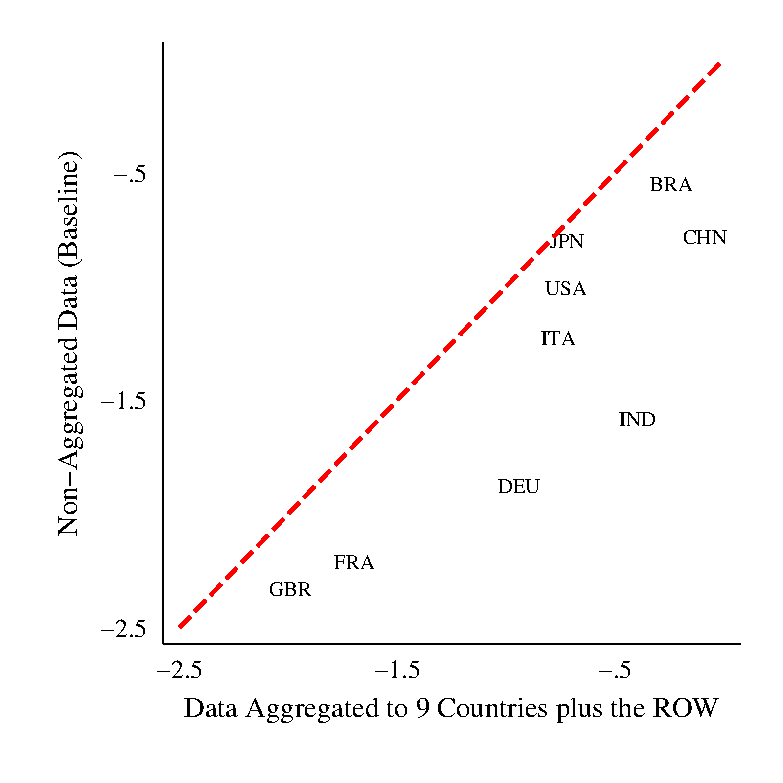
\includegraphics[scale=0.65]{Fig_4}
\end{figure}

\subsection{The Gains from Cooperative Tariffs}

The gains from cooperative tariffs can be calculated with the same
data and logic used to measure the cost of a tariff war. This procedure
capitalizes on the cooperative tariff formula specified by Equation
\ref{eq: Cooperative Tariff}. More details about implementation are
provided in Online Appendix E. As reported in Table \ref{tab: Computational-Speed},
this procedure is remarkably fast and (like the tariff war analysis)
can be seamlessly performed on data from multiple years. Without this
procedure, however, the cost of computing cooperative tariffs can
be prohibitively high given the number of countries and industries
in my analysis. 

Following the discussion in Section \ref{sec: Cooperative-Tariffs},
the gains from cooperative tariffs can be interpreted as the potential
gains from further trade talks. Figure \ref{fig: gains-from-cooperation}
plots these gains for the 2000-2014 period. The results indicate that
the potential gains from further trade talks (measured in terms of
constant real GDP) have multiplied, increasing from \$184 billion
in 2000 to \$347 billion in 2014.\footnote{In terms of percentages, the gains from cooperative tariffs have increase
from 0.21\% to 0.46\% of real GDP for the average country.} This rise is indicative of two developments: First, markup distortions
have worsened in the global economy. Second, due to the rise in international
trade, trade policies have become a more effectives second-best policy
at correcting markup distortions. This rise also suggests that the
opportunity cost of non-cooperative tariff policies has elevated to
unprecedented levels. By adopting a non-cooperative approach countries
not only expose themselves to retaliation, but also miss out on the
unexploited-but-sizable benefits of further cooperation.

\begin{figure}
\caption{\label{fig: gains-from-cooperation}The gains from cooperative tariffs
over time}

\centering{}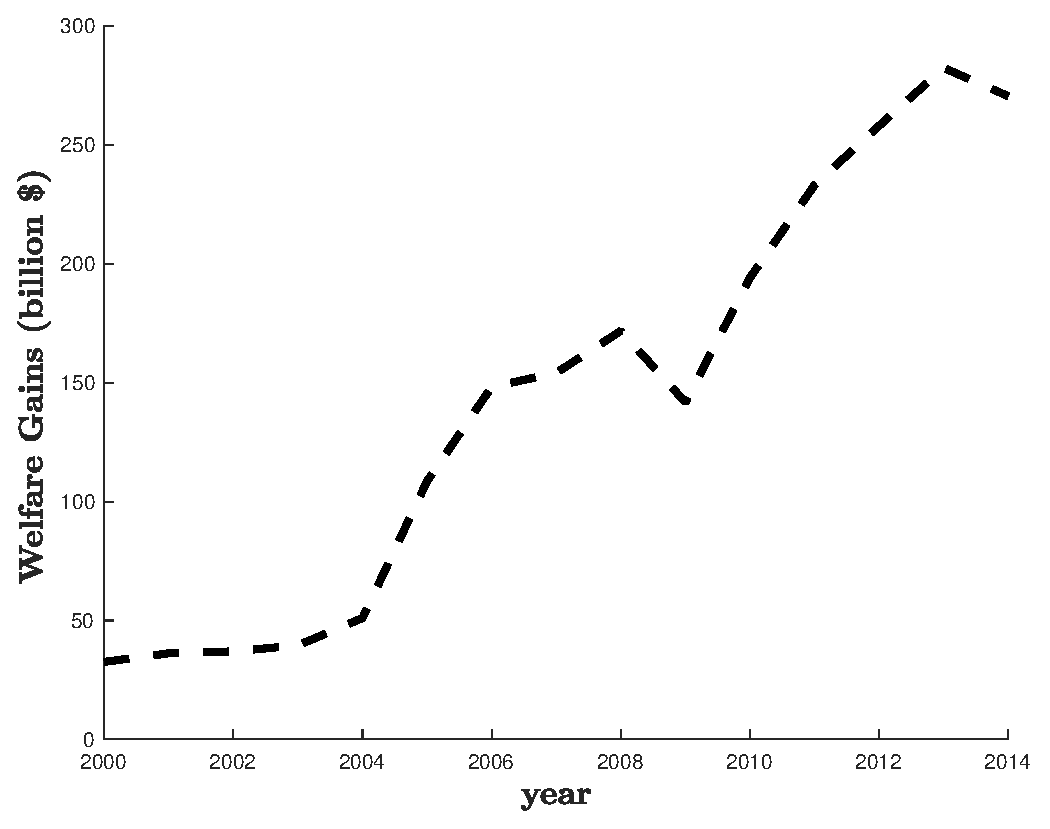
\includegraphics[scale=0.55]{Fig_5}
\end{figure}

\section{Concluding Remarks}

Building on recent advances in quantitative trade theory, I developed
a simple, sufficient statistics methodology to compute the prospective
cost of a full-fledged global tariff war. My proposed methodology
has two basic advantages. First, it derives analytic formulas for
Nash tariffs, delivering a more than 1000-fold increase in computational
speed relative to standard optimization-based approaches. Second,
it can be easily extended to account for salient features of the global
economy like input trade and pre-existing markup distortions.

I applied the new methodology to data spanning many countries, industries,
and years. This application uncovered patterns that are crucial to
the ongoing discourse surrounding trade policy: $(i)$ The prospective
cost of a global tariff war has more-than-doubled over the past 15
years; $(ii)$ a significant fraction of the cost associated with
a full-fledged tariff war is due to the exacerbation of already-existing
markup distortions; $(iii)$ small downstream economies are the most
vulnerable to a now-imminent global tariff war; and $(iv)$ \emph{cooperative}
tariffs have become a more effective tool at correcting rising markup
distortions in the global economy.

Moving forward, a natural next step is to apply the proposed methodology
to an even broader set of countries and industries using richer, confidential
data. Previously, such applications were partially impeded by computational
burden; but practitioners can employ the present methodology to circumvent
this particular obstacle. Another avenue for future research is to
extend the methodology, itself, by incorporating multiple factors
of production and other short-run adjustment costs.

\bibliographystyle{chicago}
\bibliography{Trade_War}

\let\normalsize\small 


\appendix
\newpage\small \newgeometry{left=0.75in, right=0.75in, top=1in, bottom=1in}

\section{\label{subsec: Proof Proposition-1}Proof of Proposition 1}

\subsection*{Step \#1: Express Equilibrium Variables as function of $\tilde{\textbf{P}}_{i}$,
$\textbf{w}$, and $\textbf{t}_{-i}$}

The first step of the proof is to express equilibrium variables (e.g.,
$Q_{ji,k}$, $Y_{i}$, etc.) as a function of $(1)$ the vector of
consumer prices in country $i$,
\begin{equation}
\tilde{\textbf{P}}_{i}\equiv\left\{ \tilde{P}_{ji,k}\right\} _{j,k}=\left\{ P_{1i,1},...P_{Ni,1},....,P_{1i,K},...P_{Ni,K}\right\} ;\label{eq: P_i}
\end{equation}
which recall $i$ is the country we are characterizing the unilaterally
optimal policy for;$(2)$ the vector of national-level wage rates
all over the world,
\[
\textbf{w}=\left\{ w_{1},...,w_{N}\right\} ;
\]
and $(3)$ the vector of applied tariffs in the rest of world excluding
country $i$,
\[
\textbf{t}_{-i}=\left\{ \textbf{t}_{1},...,\textbf{t}_{i-1},\textbf{t}_{i+1},...,\textbf{t}_{N}\right\} ,
\]
where $\textbf{t}_{j}=\left\{ t_{1j,1},...t_{Nj,1},....,t_{1j,K},...t_{Nj,K}\right\} $
is the vector of tariff rates applied by country $j\neq i$. Considering
the above notation, we can immediately establish the following result. 
\begin{lem}
\label{lem: Step 1}All equilibrium outcomes (excluding $\tilde{\textbf{P}}_{i}$
and $\textbf{w}$) can be uniquely determined as a function of $\textbf{t}_{-i}$,
$\tilde{\textbf{P}}_{i}$, and $\textbf{w}$.
\end{lem}
\begin{proof}
The proof follows from solving all equilibrium conditions excluding
the equilibrium expression for consumer prices, $\tilde{P}_{ji,k}$
(which pins down $\tilde{\textbf{P}}_{i}$), and the country-specific
balanced trade condition (which pins down $\textbf{w}$). Stated formally,
we need to solve the following system treating $\textbf{t}_{-i}$,
$\tilde{\textbf{P}}_{i}$, and $\textbf{w}$ as given:
\begin{align*}
P_{j\ell,k} & =a_{j\ell,k}w_{j};\ \ \ \ \ \ \ \ \ \tilde{P}_{j\iota,k}=(1+t_{j\iota,k})P_{j\iota,k}\ \ \ \iota\neq i,\ \ \ \ \ \ \ \ \ \ \ \ \ [\textrm{competitive pricing}]\\
Q_{j\ell,k} & =\mathcal{D}_{j\ell,k}(Y_{\ell},\tilde{P}_{1\ell,1},...\tilde{P}_{N\ell,1},...,\tilde{P}_{1\ell,K},...,\tilde{P}_{N\ell,K})\ \ \ \ \ \ \ \ \ \ \ \ \ [\textrm{optimal consumption}]\\
Y_{\ell}= & w_{\ell}L_{\ell}+\sum_{j\neq\ell,}\sum_{k}\left[\left(\tilde{P}_{j\ell,k}-P_{j\ell,k}\right)Q_{j\ell,k}\right]\ \ \ \ \ \ \ \ \ \ \ \ \ \ [\textrm{income = wage bill + tax revenue}]
\end{align*}
Since there is a unique equilibrium, the above system is exactly identifies
in that it uniquely determines $P_{j\ell,k}$, $Q_{j\ell,k}$, and
$Y_{\ell}$ as a function of $\textbf{t}_{-i}$, $\tilde{\textbf{P}}_{i}$,
and $\textbf{w}$ .
\end{proof}
Following Lemma \ref{lem: Step 1}, we can express total income in
country $i$, $Y_{i}$, as well as the entire demand schedule in that
country as follows:
\[
Y_{i}\equiv Y_{i}(\tilde{\textbf{P}}_{i},\textbf{t}_{-i};\textbf{w});\ \ \ \ \ \ \ \ \ \ \ Q_{ji,k}\equiv Q_{ji,k}(\tilde{\textbf{P}}_{i},\textbf{t}_{-i};\textbf{w})=\mathcal{Q}_{ji,k}\left(Y_{i}(\tilde{\textbf{P}}_{i},\textbf{t}_{-i};\textbf{w}),\tilde{\textbf{P}}_{i}\right).
\]
Recall that $\mathcal{Q}_{ji,k}(.)$ denotes the Marshallian demand
function facing variety $ji,k$. Observing the above representation,
my main objective is to reformulate country $i$'s policy problem
as one where the government chooses $\tilde{\textbf{P}}_{i}$ (as
opposed to directly choosing tariff rates) taking $\textbf{t}_{-i}$
as given. This reformulation, though, needs to take into account that
$\textbf{w}$ is an equilibrium outcome that implicitly depends on
$\textbf{t}_{-i}$ and $\tilde{\textbf{P}}_{i}$. To track this constraint,
define the $(\tilde{\textbf{P}}_{i},\textbf{t}_{-i};\textbf{w})$
combinations that are feasible as follows. 
\begin{defn}
A combination $(\tilde{\textbf{P}}_{i},\textbf{t}_{-i};\textbf{w})$
is \textbf{ \emph{feasible}} iff given $\tilde{\textbf{P}}_{i}$
and $\textbf{t}_{-i}$, the vector of wages, $\textbf{w}$, satisfies
the balanced trade condition in every country $\ell\in\mathbb{C}$.
More specifically, observing that $P_{jn}=\bar{\tau}_{jn,k}\bar{a}_{j,k}w_{j}$:\footnote{The bar notation indicates that $\bar{\tau}_{jn,k}$ and $\bar{a}_{j,k}$
are constant structural variables.}
\[
(\tilde{\textbf{P}}_{i},\textbf{t}_{-i};\textbf{w})\in\mathbb{F}\ \ \ \Longleftrightarrow\ \ \ \sum_{j\neq n}\sum_{k=1}^{K}\left[\bar{\tau}_{jn,k}\bar{a}_{j,k}w_{j}Q_{jn,k}(\tilde{\textbf{P}}_{i},\textbf{t}_{-i};\textbf{w})-\bar{\tau}_{nj,k}\bar{a}_{n,k}w_{n}Q_{nj,k}(\tilde{\textbf{P}}_{i},\textbf{t}_{-i};\textbf{w})\right]=0.
\]
Equipped with the above definition, we can now proceed with the reformulation
of the optimal policy problem (P1).
\end{defn}

\subsection*{Step \#2: Reformulate the Optimal Tariff Problem}

Recall the optimal tariff problem (P1) from Section \ref{sec:Theoretical-Framework}.
The next intermediate result shows that country $i$'s optimal tariff
problem can be cast as on where the government chooses the optimal
vector of consumer prices in the local economy instead directly choosing
the vector of tariffs.
\begin{lem}
\label{lem: Step 2}Country $i$'s vector of optimal tariffs, $\textbf{t}_{i}$,
can be determined by solving the following problem:\emph{
\[
\max_{\tilde{\textbf{P}}_{i}}\ \ W_{i}(\tilde{\textbf{P}}_{i},\textbf{t}_{-i};\textbf{w})\equiv V_{i}(Y_{i}(\tilde{\textbf{P}}_{i},\textbf{t}_{-i};\textbf{w}),\tilde{\textbf{P}}_{i})\ \ \ \ \ s.t.\ \ (\tilde{\textbf{P}}_{i},\textbf{t}_{-i};\textbf{w})\in\mathbb{F}\ \ \ \ \ \ \ (\widetilde{\textrm{P1}})
\]
}
\end{lem}
\begin{proof}
The proof proceeds in two steps. First, I show that the policy space
afforded to the government under the price vector, $\tilde{\textbf{P}}_{i}$,
is identical to that afforded under the tariff vector, $\textbf{t}_{i}=\{t_{ji,k}\}_{j\neq i,k}$.
Second, I show that the optimal choice w.r.t. $\tilde{\textbf{P}}_{i}$
implicitly and uniquely pins down the optimal choice w.r.t. $\textbf{t}_{i}$. 

\textbf{Step (a)} To set stage for the first step, note that $\textbf{t}_{i}$
is composed of $(N-1)K$ elements, whereas $\tilde{\textbf{P}}_{i}=\left\{ \tilde{\textbf{P}}_{1i},...,\tilde{\textbf{P}}_{ii},...,\tilde{\textbf{P}}_{Ni}\right\} $
is composed of $NK$ elements: namely, $(N-1)K$ import prices, $\tilde{\textbf{P}}_{-ii}$,
plus $K$ domestic prices, $\tilde{\textbf{P}}_{ii}$. Below, I show
that --because markets are competitive-- the optimal policy should
never tax good $ii,k$. This claim requires that I establish the following:
\[
\frac{\text{d}W_{i}(\tilde{\textbf{P}}_{i},\textbf{t}_{-i};\textbf{w})}{\text{d}\ln\tilde{\textbf{P}}_{ii}}=0\ \ \Longleftrightarrow\ \ \tilde{\textbf{P}}_{ii}=\textbf{P}_{ii},
\]
which entails that the optimal choice w.r.t. $\tilde{\textbf{P}}_{ii}$
of is equal to the producer price. If that is true, adding $\tilde{\textbf{P}}_{ii}$
to the government's policy choice set does not afford the government
more policy space than if the government was directly setting tariffs,
$\textbf{t}_{i}$. To prove this above claim, we can invoke the chain
rule to produce the following expression (recalling that $\tilde{\textbf{P}}_{-ii}\equiv\tilde{\textbf{P}}_{i}-\left\{ \tilde{\textbf{P}}_{ii}\right\} $):
\begin{align}
\frac{\text{d}W_{i}(.)}{\text{d}\ln\tilde{\textbf{P}}_{ii}}= & +\frac{\partial V_{i}(Y_{i},\tilde{\textbf{P}}_{i})}{\partial\ln\tilde{\textbf{P}}_{ii}}+\frac{\partial V_{i}(Y_{i},\tilde{\textbf{P}}_{i})}{\partial Y_{i}}\left(\frac{\partial Y_{i}}{\partial\ln\tilde{\textbf{P}}_{ii}}\right)_{\textbf{w},\ \textbf{t}_{-i},\ \tilde{\textbf{P}}_{-ii}}+\left(\frac{\partial W_{i}(.)}{\partial\textbf{w}}\right)_{\textbf{t}_{-i},\ \tilde{\textbf{P}}_{i}}\left(\frac{\text{d}\textbf{w}}{\text{d}\ln\tilde{\textbf{P}}_{ii}}\right)_{\textbf{t}_{-i},\ \tilde{\textbf{P}}_{-ii}}.\label{eq: dW/dP_ii}
\end{align}
By Roy's identity, the first term on the right-hand side can be formulated
as
\[
\hspace{-0.75in}[\textrm{Roy's identity}]\ \ \ \ \ \ \ \ \ \ \ \ \ \ \ \ \ \ \ \ \frac{\partial V_{i}(Y_{i},\tilde{\textbf{P}}_{i})}{\partial\ln\tilde{\textbf{P}}_{ii}}=-\tilde{\textbf{P}}_{ii}\cdot\textbf{Q}_{ii},
\]
where the operator ``$\cdot$'' corresponds to the inner product
of two vectors. The second term on the right-hand side in Equation
\ref{eq: dW/dP_ii} can be determined by taking a derivative w.r.t.
$\tilde{\textbf{P}}_{ii}$ from the balanced budget condition, $Y_{i}=w_{i}L_{i}+\sum_{j=1}^{N}\left(\tilde{\textbf{P}}_{ji}-\textbf{P}_{ji}\right)\cdot\textbf{Q}_{ji}$,
which yields\footnote{To be clear: $\sum_{j=1}^{N}\left(\tilde{\textbf{P}}_{ji}-\textbf{P}_{ji}\right)\cdot\textbf{Q}_{ji}=\sum_{j=1}^{N}\sum_{k=1}^{K}\left[\left(\tilde{P}_{ji,k}-P_{ji,k}\right)Q_{ji,k}\right]$
by definition of the inner product operator, ``$\cdot$''.}
\[
\frac{\partial V_{i}(Y_{i},\tilde{\textbf{P}}_{i})}{\partial Y_{i}}\left(\frac{\partial Y_{i}}{\partial\ln\tilde{\textbf{P}}_{ii}}\right)_{\textbf{w},\ \textbf{t}_{-i},\ \tilde{\textbf{P}}_{-ii}}=\tilde{\textbf{P}}_{ii}\cdot\textbf{Q}_{ii}+\left(\tilde{\textbf{P}}_{ii}-\textbf{P}_{ii}\right)\cdot\left(\frac{\partial\textbf{Q}_{ii}}{\partial\ln\tilde{\textbf{P}}_{ii}}\right)_{\textbf{w},\ \textbf{t}_{-i},\ \tilde{\textbf{P}}_{-ii}}.
\]
The last term on the right-hand side of Equation \ref{eq: dW/dP_ii}
is also equal to zero: $\left(\frac{\text{d}\textbf{w}}{\text{d}\ln\tilde{\textbf{P}}_{ii}}\right)_{\textbf{t}_{-i},\ \tilde{\textbf{P}}_{-ii}}=0$,
since demand is homogenous of degree zero. Combining these expressions
and plugging them back into Equation \ref{eq: dW/dP_ii} establishes
that
\[
\frac{\text{d}W_{i}(.)}{\text{d}\ln\tilde{\textbf{P}}_{ii}}=\left(\tilde{\textbf{P}}_{ii}-\textbf{P}_{ii}\right)\cdot\left(\frac{\partial\textbf{Q}_{ii}}{\partial\ln\tilde{\textbf{P}}_{ii}}\right)_{\textbf{w},\ \textbf{t}_{-i},\ \tilde{\textbf{P}}_{i}-\left\{ \tilde{\textbf{P}}_{ii}\right\} }=0\ \ \Longleftrightarrow\ \ \tilde{\textbf{P}}_{ii}=\textbf{P}_{ii}.
\]

\textbf{Step (b)} It is straightforward to verify that there is
a one-to-one correspondence between the optimal choice w.r.t. $\tilde{\textbf{P}}_{-ii}\equiv\tilde{\textbf{P}}_{i}-\left\{ \tilde{\textbf{P}}_{ii}\right\} $
and $\textbf{t}_{i}$. More specifically the optimal choice w.r.t.
$\tilde{\textbf{P}}_{-ii}$ implicitly pins down the entire vector
of optimal tariffs as
\[
\left\{ 1+t_{1i,1}^{*},...,1+t_{Ni,1}^{*},...,1+t_{1i,K}^{*},...,1+t_{Ni,K}^{*}\right\} =\left\{ \frac{\tilde{P}_{1i,1}^{*}}{P_{1i,1}},...,\frac{\tilde{P}_{Ni,1}^{*}}{P_{Ni,1}},...,\frac{\tilde{P}_{1i,K}^{*}}{P_{1i,K}},...,\frac{\tilde{P}_{Ni,K}^{*}}{P_{Ni,K}}\right\} .
\]
Put differently, there is always unique vector of tariffs that can
implement the optimal import price vector, $\tilde{\textbf{P}}_{-ii}^{*}$.
Together, Steps $(i)$ and $(ii)$ establish the equivalence between
Problems (P1) and ($\widetilde{\textrm{P1}}$).
\end{proof}

\subsection*{Step \#3: Solving the System of F.O.C.'s Associated with $\widetilde{\textrm{P1}}$}

This step derives and solves the system of F.O.C.s associated with
Problem $\widetilde{\textrm{P1}}$. I will adopt the dual approach
in this process, which relies heavily on Marshallian demand elasticities.
So, to fix ideas and avoid any confusion later on, I formally define
these elasticities in the following.

\paragraph*{Notation A {[}\emph{Marshallian} Demand Elasticities{]}}

\emph{Let }$Q_{ji,k}\equiv\mathcal{Q}_{ji,k}(Y_{i},\tilde{\textbf{P}}_{i})$
\emph{denote the Marshallian demand function facing variety $ji,k$.
This demand function is characterized by the following reduced-form
demand elasticities:
\[
[\textrm{price elasticity}]\ \ \ \ \varepsilon_{ji,k}^{(ni,g)}\equiv\frac{\partial\ln\mathcal{Q}_{ji,k}(Y_{i},\tilde{\textbf{P}}_{i})}{\partial\ln\tilde{P}_{ni,g}}
\]
\[
[\textrm{income elasticity}]\ \ \ \ \eta_{ji,k}\equiv\frac{\partial\ln\mathcal{Q}_{ji,k}(Y_{i},\tilde{\textbf{P}}_{i})}{\partial\ln Y_{i}},
\]
where }$\tilde{\textbf{P}}_{i}$ \emph{corresponds to the entire of
vector of consumer prices in market $i$ as specified by \ref{eq: P_i}.
Recall} \emph{from the main text that }$V(Y_{i},\tilde{\textbf{P}}_{i})$\emph{
denotes the indirect utility associated with the Marshallian demand
function,} $\mathcal{Q}_{ji,k}(Y_{i},\tilde{\textbf{P}}_{i})$\emph{.}

The general equilibrium problem we are analyzing has many free-moving
components. So, when taking partial derivative it is important to
specify the variables that are being held constant. At the same, I
would like to maintain a compact notation. So, for future reference,
the following clarifies my choice of notation w.r.t. partial derivatives.

\paragraph*{Notation B {[}Partial derivatives{]}}

\emph{Since the vector of tariffs in the rest of the world,} $\textbf{t}_{-i}$\emph{,
is treated as given and the elements of }$\tilde{\textbf{P}}_{i}$\emph{
are treated as policy choices, the partial derivative of variable
}$x\equiv x(\tilde{\textbf{P}}_{i},\textbf{t}_{-i};\textbf{w})$\emph{
w.r.t. }$\tilde{P}_{ji,k}\in\tilde{\textbf{P}}_{i}$\emph{ should
be interpreted as a partial derivative holding }$\textbf{t}_{-i}$
\emph{and }$\tilde{\textbf{P}}_{i}-\left\{ \tilde{P}_{ji,k}\right\} $\emph{
fixed. Namely,}
\[
\frac{\partial x}{\partial\ln\tilde{P}_{ji,k}}\equiv\left(\frac{\partial x}{\partial\ln\tilde{P}_{ji,k}}\right)_{\tilde{\textbf{P}}_{i}-\left\{ \tilde{P}_{ji,k}\right\} ,\ \textbf{t}_{-i}};\ \ \ \ \ \ \ \ \ \ \ \left(\frac{\partial x(.)}{\partial\ln\tilde{P}_{ji,k}}\right)_{\textbf{w}}\equiv\left(\frac{\partial x(.)}{\partial\ln\tilde{P}_{ji,k}}\right)_{\textbf{w},\ \tilde{\textbf{P}}_{i}-\left\{ \tilde{P}_{ji,k}\right\} ,\ \textbf{t}_{-i}}.
\]
Considering Lemma \ref{lem: Step 2} and the notation outlined above,
we can write the system of F.O.C.'s underlying Problem $\widetilde{\textrm{P1}}$
as
\[
\nabla_{\tilde{\textbf{P}}_{i}}W_{i}(\tilde{\textbf{P}}_{i},\textbf{t}_{-i};\textbf{w})=\textbf{0}.
\]
Using the cain rule, the F.O.C. w.r.t. $\tilde{P}_{ji,k}\in\tilde{\textbf{P}}_{i}$,
in particular, can be stated as follows:
\begin{align}
\frac{\text{d}W_{i}(.)}{\text{d}\ln\tilde{P}_{ji,k}} & =\frac{\partial V_{i}(.)}{\partial\ln\tilde{P}_{ji,k}}+\frac{\partial V_{i}(.)}{\partial Y_{i}}\left(\frac{\partial Y_{i}}{\partial\ln\tilde{P}_{ji,k}}\right)_{\textbf{w}}+\left(\frac{\partial W_{i}(.)}{\partial\ln\textbf{w}}\right)_{\tilde{\textbf{P}}_{i}}\cdot\frac{\text{d}\ln\textbf{w}}{\text{d}\ln\tilde{P}_{ji,k}}\nonumber \\
 & =\frac{\partial V_{i}}{\partial Y_{i}}\left(\frac{\partial V_{i}(.)}{\partial\ln\tilde{P}_{ji,k}}\left(\frac{\partial V_{i}}{\partial Y_{i}}\right)^{-1}+\left(\frac{\partial Y_{i}}{\partial\ln\tilde{P}_{ji,k}}\right)_{\textbf{w}}+\left(\frac{\partial W_{i}(.)}{\partial\ln\textbf{w}}\right)_{\tilde{\textbf{P}}_{i}}\cdot\frac{\text{d}\ln\textbf{w}}{\text{d}\ln\tilde{P}_{ji,k}}\left(\frac{\partial V_{i}}{\partial Y_{i}}\right)^{-1}\right)=0\label{eq: FOC (fh,k)}
\end{align}
To elaborate, the first two terms in Equation \ref{eq: FOC (fh,k)}
correspond to the change in $W_{i}$ holding $\textbf{w}$ fixed.
The last term accounts for general equilibrium wage effects. In particular,
$\left(\partial W_{i}(.)/\partial\ln\textbf{w}\right)_{\tilde{\textbf{P}}_{i}}$
corresponds to the pure effect of wages, $\textbf{w}$, on welfare,
$W_{i}$, holding all elements of $\tilde{\text{P}}_{i}$ and $\textbf{t}_{-i}$
fixed. The term $\text{d}\ln\textbf{w}/\text{d}\ln\tilde{P}_{ji,k}$
corresponds to the change in $\textbf{w}$ in response to a change
in $\tilde{P}_{ji,k}$ (holding $\textbf{t}_{-i}$ \emph{and }$\tilde{\textbf{P}}_{i}-\left\{ \tilde{P}_{ji,k}\right\} $\emph{
}fixed). Following Lemma \ref{lem: Step 2}, $\text{d}\ln\textbf{w}/\text{d}\ln\tilde{P}_{ji,k}$
is pinned down by the \emph{balanced trade condition}.

The first term in Equation \ref{eq: FOC (fh,k)}, which reflects the
direct effect of prices on welfare, can be characterized using Roy's
identity. Specifically noting that $V_{i}(.)\equiv V_{i}(Y_{i},\tilde{\textbf{P}}_{i})$,
the optimal consumption choice entails that
\begin{equation}
[\textrm{Roy's identity}]\ \ \ \ \ \ \ \ \ \ \left(\frac{\partial V_{i}(.)}{\partial Y_{i}}\right)^{-1}\frac{\partial V_{i}(.)}{\partial\ln\tilde{P}_{ji,k}}=-\tilde{P}_{ji,k}Q_{ji,k}.\label{eq: Price Effect}
\end{equation}
The second term in Equation \ref{eq: FOC (fh,k)}, which encompasses
income effects holding $\textbf{w}$ fixed, can be determined by taking
a partial derivative w.r.t. to the balanced budget condition, which
can be expressed as follows given that $t_{ni,g}=\tilde{P}_{ni,g}-P_{ni,g}$:
\begin{align}
Y_{i}=w_{i}L_{i}+\sum_{n\neq i,}\sum_{g=1}^{K}\left[\left(\tilde{P}_{ni,g}-P_{ni,g}\right)Q_{ni,g}\right] & .\label{eq: Budget Constraint}
\end{align}
Observe that $\tilde{P}_{in,g}\in\tilde{\textbf{P}}_{i}$ for all
$ni,g$ and that $P_{ni,g}=\bar{\tau}_{ni,g}\bar{a}_{n,g}w_{n}$.
Taking the partial derivative of Equation \ref{eq: Budget Constraint}
w.r.t. $\tilde{P}_{ji,k}$ yields the following expression
\begin{equation}
\left(\frac{\partial Y_{i}(\tilde{\textbf{P}}_{i},\textbf{t}_{-i};\textbf{w})}{\partial\ln\tilde{P}_{ji,k}}\right)_{\textbf{w}}=\tilde{P}_{ji,k}Q_{ji,k}+\sum_{n\neq i}\sum_{g}\left[\left(\tilde{P}_{ni,g}-P_{ni,g}\right)Q_{ni,g}\left(\frac{\partial\ln Q_{ni,g}(.)}{\partial\ln\tilde{P}_{ji,k}}\right)_{\textbf{w}}\right],\label{eq: Income Effect}
\end{equation}
where the optimality of final demand entails that adjustments to demand
are regulated by the Marshallian demand elasticities:
\begin{align*}
\left(\frac{\partial\ln Q_{ni,g}(.)}{\partial\ln\tilde{P}_{ji,,k}}\right)_{\textbf{w}}=\frac{\partial\ln\mathcal{Q}_{ni,g}(Y_{i},\tilde{\textbf{P}}_{i})}{\partial\ln\tilde{P}_{ji,k}} & +\frac{\partial\ln\mathcal{Q}_{ni,g}(Y_{i},\tilde{\textbf{P}}_{i})}{\partial\ln Y_{i}}\left(\frac{\partial Y_{i}(.)}{\partial\ln\tilde{P}_{ji,k}}\right)_{\textbf{w}}=\varepsilon_{ni,g}^{(ji,k)}+\eta_{ni,g}\left(\frac{\partial Y_{i}(.)}{\partial\ln\tilde{P}_{ji,k}}\right)_{\textbf{w}}.
\end{align*}
Plug the above expression back into Equation \ref{eq: Income Effect}
and use the inner product ``$\cdot$'' and vector calculus to economize
on the notation. We can, thus, express the direct income effects (featured
in Equation \ref{eq: FOC (fh,k)}) as follows
\[
\left(\frac{\partial Y_{i}(\tilde{\textbf{P}}_{i},\textbf{t}_{-i};\textbf{w})}{\partial\ln\tilde{P}_{ji,k}}\right)_{\textbf{w}}=\tilde{P}_{ji,k}Q_{ji,k}+\sum_{n\neq i}\left[\left(\tilde{\textbf{P}}_{ni}-\textbf{P}_{ni}\right)\cdot\textbf{Q}{}_{ni}\odot\left(\boldsymbol{\varepsilon}_{ni}^{(ji,k)}+\boldsymbol{\eta}_{ni}\left(\frac{\partial Y_{i}(.)}{\partial\ln\tilde{P}_{ji,k}}\right)_{\textbf{w}}\right)\right],
\]
where $\boldsymbol{\varepsilon}_{ni}^{(ji,k)}\equiv\left[\varepsilon_{ni,g}^{(ji,k)}\right]_{g}$
is a $K\times1$ vector denoting the price elasticity of all imported
varieties from origin $n$ w.r.t. $\tilde{P}_{ji,k}$, $\boldsymbol{\eta}_{ni}\equiv\left[\eta_{ni,g}\right]_{g}$
is a $K\times1$ vector denoting the income elasticity of demand facing
these varieties. The operator $\odot$ represents element-wise multiplication:
$\text{a}\odot\textbf{b}=[a_{i}b_{i}]_{i}$. 

Assign wage in country $j$ as the numeraire: $w_{j}=1$. The last
term in Equation \ref{eq: FOC (fh,k)} can be decomposed as
\[
\frac{\partial W_{i}(.)}{\partial\ln\textbf{w}}\frac{\text{d}\ln\textbf{w}}{\text{d}\ln\tilde{P}_{ji,k}}\left(\frac{\partial V_{i}}{\partial Y_{i}}\right)^{-1}=\left[\left(\frac{\partial W_{i}}{\partial\ln w_{i}}\right)_{\textbf{w}_{-i}}\frac{\text{d}\ln w_{i}}{\text{d}\ln\tilde{P}_{ji,k}}+\left(\frac{\partial W_{i}}{\partial\ln\textbf{w}_{-i}}\right)_{w_{i}}\cdot\frac{\text{d}\ln\textbf{w}_{-i}}{\text{d}\ln\tilde{P}_{ji,k}}\right]\left(\frac{\partial V_{i}}{\partial Y_{i}}\right)^{-1}
\]
Following the discussion in Appendix \ref{sec: Welfare-Approximation},
after assigning $w_{j}$ as the numeriare, $\left(\frac{\partial W_{i}}{\partial\ln\textbf{w}_{-i}}\right)_{w_{i}}\cdot\frac{\text{d}\ln\textbf{w}_{-i}}{\text{d}\ln\tilde{P}_{ji,k}}=0$
to a first-order approximation if $r_{ni,k}/r_{ii,k}\approx0$ for
$n\neq i$. So, by choice of numeraire, we can treat $\bar{\textbf{w}}_{-i}$
as fixed hereafter---see Appendix \ref{sec: Assumption on Size}
for a derivation of optimal tariffs without this approximation. Importantly,
though, the choice of $\tilde{P}_{ji,k}$ has a non-trivial effect
on the ratio of $w_{i}$ relative to $\textbf{w}_{-i}$. This effect,
which is represented by $\text{d}\ln w_{i}/\text{d}\ln\tilde{P}_{ji,k}$,
can be evaluated by applying the Implicit Function Theorem to the
balanced trade condition in country $i$,
\begin{align*}
\mathrm{T}_{i}(\tilde{\textbf{P}}_{i},\textbf{t}_{-i};w_{i},\textbf{w}_{-i})\equiv & \sum_{n\neq i}\left[\textbf{P}_{ni}\cdot\textbf{Q}_{ni}-\textbf{P}_{in}\cdot\textbf{Q}_{in}\right]\\
= & \sum_{k}\sum_{n\ne i}\left[\bar{\tau}_{ni,k}\bar{a}_{n,k}w_{n}Q_{ni,k}(\tilde{\textbf{P}}_{i},\textbf{t}_{-i};\textbf{w})-\bar{\tau}_{in,k}\bar{a}_{i,k}w_{i}Q_{in,k}(\tilde{\textbf{P}}_{i},\textbf{t}_{-i};\textbf{w})\right]=0
\end{align*}
while treating $\textbf{w}_{-i}=\bar{\textbf{w}}_{-i}$ as given.
This step yields the following equation
\begin{equation}
\left(\frac{\text{d}\ln w_{i}}{\text{d}\ln\tilde{P}_{ji,k}}\right)_{\bar{\textbf{w}}_{-i}}=\dfrac{-\left(\frac{\partial\mathrm{T}_{i}(\tilde{\textbf{P}}_{i},\textbf{t}_{-i};w_{i},\bar{\textbf{w}}_{-i})}{\partial\ln\tilde{P}_{ji,k}}\right)_{\textbf{w}}}{\left(\frac{\partial\mathrm{T}_{i}(\tilde{\textbf{P}}_{i},\textbf{t}_{-i};w_{i},\bar{\textbf{w}}_{-i})}{\partial\ln w_{i}}\right)_{\bar{\textbf{w}}_{-i}}}=\frac{-\sum_{n\neq i}\left[\textbf{P}_{ni}\cdot\left(\frac{\partial\ln\textbf{Q}_{ni}(.)}{\partial\ln\tilde{P}_{ji,k}}\right)_{\textbf{w}}\right]}{\left(\frac{\partial\mathrm{T}_{i}(\tilde{\textbf{P}}_{i},\textbf{t}_{-i};w_{i},\bar{\textbf{w}}_{-i})}{\partial\ln w_{i}}\right)_{\bar{\textbf{w}}_{-i}}}.\label{eq: dw/dP PC}
\end{equation}
The second line follows from the fact that $\left(\frac{\partial\ln Q_{in,g}(.)}{\partial\ln\tilde{P}_{ji,k}}\right)_{\textbf{w}}=0$
if $n\neq i$. That is, if we fix the vector of wages, $\textbf{w}$,
the choice of $\tilde{P}_{ji,k}$ has no effect on the demand schedule
in the rest of the world. The only way the effect of $\tilde{P}_{ji,k}$
travels to foreign markets is through its effect on $\textbf{w}$.
Define the importer-wide term,
\[
\bar{\tau}_{i}\equiv\frac{\frac{\partial W_{i}(.)/\partial\ln w_{i}}{\partial V_{i}(.)/\partial Y_{i}}}{\left(\partial\mathrm{T}_{i}(.)/\partial\ln w_{i}\right)_{\bar{\textbf{w}}_{-i}}},
\]
and note that $\bar{\tau}_{i}$ does not feature an industry-specific
subscript. Using Equation \ref{eq: dw/dP PC} and the definition for
$\bar{\tau}_{i}$, the last term in F.O.C. (Equation \ref{eq: FOC (fh,k)})
become{\footnotesize{}s
\begin{align}
\left(\frac{\partial W_{i}}{\partial\ln\textbf{w}}\right)_{\tilde{\textbf{P}}_{i}}\cdot\frac{\text{d}\ln\textbf{w}}{\text{d}\ln\tilde{P}_{ji,k}} & \left(\frac{\partial V_{i}}{\partial Y_{i}}\right)^{-1}=\frac{\partial W_{i}}{\partial\ln w_{i}}\frac{\text{d}\ln w_{i}}{\text{d}\ln\tilde{P}_{ji,k}}\left(\frac{\partial V_{i}}{\partial Y_{i}}\right)^{-1}=-\bar{\tau}_{i}\left(\frac{\partial\mathrm{T}_{i}(.)}{\partial\ln\tilde{P}_{ji,k}}\right)_{\textbf{w}}\nonumber \\
 & =-\bar{\tau}_{i}\sum_{n\neq i}\left[\textbf{P}_{ij}\cdot\left(\frac{\partial\ln\textbf{Q}_{ij}(.)}{\partial\ln\tilde{P}_{ji,k}}\right)_{\textbf{w}}\right]=-\bar{\tau}_{i}\sum_{n\neq i}\left[\textbf{P}_{ni}\cdot\textbf{Q}{}_{ni}\odot\left(\boldsymbol{\varepsilon}_{-ii}^{(ji,k)}+\boldsymbol{\eta}_{-ii}\left(\frac{\partial Y_{i}(.)}{\partial\ln\tilde{P}_{ji,k}}\right)_{\textbf{w}}\right)\right].\label{eq: Wage Effect}
\end{align}
}Plugging Equations \ref{eq: Income Effect}, \ref{eq: Price Effect},
and \ref{eq: Wage Effect} back into the F.O.C. specified by Equation
\ref{eq: FOC (fh,k)}), yields the following necessary condition for
optimality:
\begin{align*}
\sum_{n\neq i}\left[\left(\tilde{\textbf{P}}_{ni,g}-(1+\bar{\tau}_{i})\textbf{P}_{ni,g}\right)\cdot\textbf{Q}_{ni}\odot\boldsymbol{\varepsilon}_{ni}^{(ji,k)}\right]+\sum_{n\neq i}\left[\left(\tilde{\textbf{P}}_{ni,g}-(1+\bar{\tau}_{i})\textbf{P}_{ni,g}\right)\cdot\textbf{Q}_{ni}\odot\boldsymbol{\eta}_{ni}\right]\left(\frac{\partial Y_{i}}{\partial\ln\tilde{P}_{ji,k}}\right)_{\textbf{w}} & =0
\end{align*}
Given that demand is homogeneous of degree zero, it is immediate that
the solution to the above system should satisfy
\begin{equation}
\sum_{n\neq i}\left[\left(\tilde{\textbf{P}}_{ni,g}-(1+\bar{\tau}_{i})\textbf{P}_{ni,g}\right)\cdot\textbf{Q}_{ni}\odot\boldsymbol{\varepsilon}_{ni}^{(ji,k)}\right]=0\ \ \ \ \ \ \forall ji,k\neq ii,k.\label{eq: FOC PC}
\end{equation}
To solve the above system of equations, we can be stated in matrix
form as follows (refer to Section \ref{sec:Theoretical-Framework}
for the definition of $e_{ni,k}$)
\[
\underbrace{\left[\begin{array}{ccccccc}
e_{1i,1}\varepsilon_{1i,1}^{(1i,1)} & \cdots & e_{Ni,}\varepsilon_{Ni,1}^{(1i,1)} & \cdots & e_{1i,K}\varepsilon_{1i,K}^{(1i,1)} & \cdots & e_{Ni,K}\varepsilon_{Ni,K}^{(1i,1)}\\
\vdots & \ddots &  & \ddots &  & \ddots & \vdots\\
e_{1i,1}\varepsilon_{1i,1}^{(Ni,K)} & \cdots & e_{Ni,}\varepsilon_{Ni,1}^{(Ni,K)} & \cdots & e_{1i,K}\varepsilon_{1i,K}^{(Ni,K)} & \cdots & e_{Ni,K}\varepsilon_{Ni,K}^{(Ni,K)}
\end{array}\right]}_{\tilde{\textbf{E}}_{i}}\left[\begin{array}{c}
1-\left(1+\bar{\tau}_{i}\right)\frac{P_{1i,1}}{\tilde{P}_{1i,k}^{*}}\\
\vdots\\
1-\left(1+\bar{\tau}_{i}\right)\frac{P_{Ni,K}}{\tilde{P}_{Ni,K}^{*}}
\end{array}\right]=\textbf{0}.
\]
The final step is to show that the unique solution to the above system
is the trivial solution. The following lemma establishes this property.
\begin{lem}
Matrix $\textbf{E}_{i}$ is non-singular, so that $\textbf{E}_{i}\textbf{X}_{(N-1)K\times1}=0$
$\Longleftrightarrow$ $\textbf{X}_{(N-1)K\times1}=0$.
\end{lem}
\begin{proof}
Following Proposition 2.E.2 in \citet{mas1995microeconomic} the Marshallian
demand elasticities satisfies the Cournot aggression. So, observing
that $\varepsilon_{ji,k}^{(ji,k)}<-1$ and $\varepsilon_{ji,k}^{(ni,g)}>0$,
we can deduce the following:
\[
[\textrm{Cournot aggregation}]\ \ \ \ \ \ \ e_{ji,k}+\sum_{n}\sum_{g}e_{ni,g}\varepsilon_{ni,g}^{(ji,k)}=0\ \ \Longrightarrow\ \ \mid e_{ji,k}\varepsilon_{ji,k}^{(ji,k)}\mid=e_{ji,k}+\sum_{n\neq i}\sum_{g}\mid e_{ni,g}\varepsilon_{ni,g}^{(ji,k)}\mid
\]
Since, by definition, there exists a $ji,k$ for which $e_{ji,k}>0$,
the matrix $\textbf{E}_{i}$ is strictly diagonally dominant, i.e.,
\[
\exists\ jk\ \colon\ \left|\left[\textbf{E}_{i}\right]_{jk,jk}\right|>\sum_{ng\in\mathbb{N\times\mathbb{K}}-\left\{ jk\right\} }\left|\left[\textbf{E}_{i}\right]_{jk,ng}\right|
\]
The L\`evy-Desplanques Theorem (\citet{horn2012matrix}), therefore,
ensures that $\textbf{\textbf{E}}_{i}$ is non-singular. The non-singularity
of $\textbf{\textbf{E}}_{i}$ trivially implies that the unique solution
to the system, $\textbf{E}_{i}\textbf{X}_{(N-1)K\times1}=0$, is the
trivial solution, $\textbf{X}_{(N-1)K\times1}=0$.
\end{proof}
Following Lemma 4, the unique solution that satisfies the system of
F.O.C.s associated with $\widetilde{\textrm{P1}}$ is $1-\left(1+\bar{\tau}_{i}\right)\frac{P_{ji,1}}{\tilde{P}_{ji,k}^{*}}=0$
for all $j\neq i$ and $k$. Noting from Lemma \ref{lem: Step 2}
that $\tilde{P}_{ji,k}^{*}/P_{ji,k}=1+t_{ji,k}^{*}$, the unique solution
to the system of F.O.C.'s characterizing the optimal tariff problem
(P1) is a uniform tariff equal to $\bar{\tau}_{i}$:
\begin{equation}
t_{ji,k}^{*}=t_{i}^{*}=\bar{\tau}_{i},\ \ \ \ \ \ \ \ \ \ \ \ \ \ \ \ \forall j\neq i,\ \ k.\label{eq: t*}
\end{equation}


\subsection*{Step \#4: Characterizing $\bar{\tau}_{i}$}

The final step in characterizing the optimal tariff is to determine,
$\bar{\tau}_{i}$, which recall is defined as
\begin{equation}
\bar{\tau}_{i}\equiv\frac{\frac{\left(\partial W_{i}(.)/\partial\ln w_{i}\right)_{\bar{\textbf{w}}_{-i}}}{\partial V_{i}(.)/\partial Y_{i}}}{\left(\partial\mathrm{T}_{i}(.)/\partial\ln w_{i}\right)_{\bar{\textbf{w}}_{-i}}}\sim\frac{\frac{\left(\partial W_{i}(.)/\partial\ln w_{i}\right)_{\tilde{\textbf{P}}_{i},\textbf{t}_{-i},\bar{\textbf{w}}_{-i}}}{\partial V_{i}(.)/\partial Y_{i}}}{\left(\partial\mathrm{T}_{i}(.)/\partial\ln w_{i}\right)_{\tilde{\textbf{P}}_{i},\textbf{t}_{-i},\bar{\textbf{w}}_{-i}}}.\label{eq: tau_i}
\end{equation}
The numerator in Equation \ref{eq: tau_i} can characterized along
the following steps{\footnotesize{}
\begin{align*}
\hspace{-0.25in}\frac{\left(\partial W_{i}(.)/\partial\ln w_{i}\right)_{\tilde{\textbf{P}}_{i},\textbf{t}_{-i},\bar{\textbf{w}}_{-i}}}{\partial V_{i}(.)/\partial Y_{i}} & =\frac{\partial V_{i}(.)/\partial Y_{i}}{\partial V_{i}(.)/\partial Y_{i}}\left(\frac{\partial Y_{i}}{\partial\ln w_{i}}\right)_{\tilde{\textbf{P}}_{i},\textbf{t}_{-i},\bar{\textbf{w}}_{-i}}=w_{i}L_{i}-\left(\frac{\partial}{\partial\ln w_{i}}\sum_{n}\left(\tilde{\textbf{P}}_{ni}-\textbf{P}_{ni}\right)\cdot\textbf{Q}_{ni}\right)_{\tilde{\textbf{P}}_{i},\textbf{t}_{-i},\bar{\textbf{w}}_{-i}}\\
\hspace{-0.25in} & =w_{i}L_{i}-\textbf{P}_{ii}\cdot\textbf{Q}_{ii}+\sum_{j\neq i}\left[\left(\tilde{\textbf{P}}_{ji}-\textbf{P}_{ji}\right)\cdot\left(\frac{\textbf{\ensuremath{\partial}Q}_{ji}}{\partial\ln w_{i}}\right)_{\tilde{\textbf{P}}_{i},\textbf{t}_{-i},\bar{\textbf{w}}_{-i}}\right]=w_{i}L_{i}-\textbf{P}_{ii}\cdot\textbf{Q}_{ii}+\bar{\tau}_{i}\textbf{P}_{-ii}\cdot\left(\frac{\textbf{\ensuremath{\partial}Q}_{-ii}}{\partial\ln w_{i}}\right)_{\tilde{\textbf{P}}_{i},\textbf{t}_{-i},\bar{\textbf{w}}_{-i}},
\end{align*}
}where recall that ``$\cdot$'' denotes the inner product, with
$\textbf{P}_{ji}\equiv\left\{ \tilde{P}_{ji,k}\right\} _{k}$ and
$\textbf{P}_{-ii}\equiv\left\{ \textbf{P}_{ji}\right\} _{j\neq i}$.
The last line in the above equation follows from the fact that the
optimal tariff choice entails that $\tilde{\textbf{P}}_{-ii}-\textbf{P}_{-ii}=\bar{\tau}_{i}\textbf{P}_{-ii}$.
Likewise, the denominator in Equation \ref{eq: tau} can be specified
as follows:{\small{}
\[
\hspace{-0.25in}\left(\frac{\partial\mathrm{T}_{i}(.)}{\partial\ln w_{i}}\right)_{\tilde{\textbf{P}}_{i},\textbf{t}_{-i},\bar{\textbf{w}}_{-i}}=\left(\frac{\partial}{\partial\ln w_{i}}\sum_{j\neq i}\left[\tilde{\textbf{P}}_{ji}\cdot\textbf{Q}_{ji}-\tilde{\textbf{P}}_{ij}\cdot\textbf{Q}_{ij}\right]\right)_{\tilde{\textbf{P}}_{i},\textbf{t}_{-i},\bar{\textbf{w}}_{-i}}=\textbf{P}_{-ii}\cdot\left(\frac{\textbf{\ensuremath{\partial}Q}_{-ii}}{\partial\ln w_{i}}\right)_{\tilde{\textbf{P}}_{i},\textbf{t}_{-i},\bar{\textbf{w}}_{-i}}-\sum_{j\neq i}\left[\left(\frac{\partial\textbf{P}_{ij}\cdot\textbf{Q}_{ij}}{\partial\ln w_{i}}\right)_{\tilde{\textbf{P}}_{i},\textbf{t}_{-i},\bar{\textbf{w}}_{-i}}\right].
\]
}Plugging the above expressions back into Equation \ref{eq: tau}
yields the following:
\begin{align}
\bar{\tau}_{i}=\frac{w_{i}L_{i}-\textbf{P}_{ii}\cdot\textbf{Q}_{ii}+\bar{\tau}_{i}\textbf{P}_{-ii}\cdot\left(\frac{\textbf{\ensuremath{\partial}Q}_{-ii}}{\partial\ln w_{i}}\right)_{\tilde{\textbf{P}}_{i},\textbf{t}_{-i}}}{\textbf{P}_{-ii}\left(\frac{\textbf{\ensuremath{\partial}Q}_{-ii}}{\partial\ln w_{i}}\right)_{\tilde{\textbf{P}}_{i},\textbf{t}_{-i}}-\sum_{j\neq i}\left[\textbf{P}_{ij}\odot\textbf{Q}_{ij}\cdot\left(\frac{\partial\ln\textbf{P}_{ij}\odot\textbf{Q}_{ij}}{\partial\ln w_{i}}\right)_{\tilde{\textbf{P}}_{i},\textbf{t}_{-i},\bar{\textbf{w}}_{-i}}\right]}=\frac{-1}{\sum_{j\neq i}\left[\textbf{X}_{ij}\cdot\left(\frac{\partial\ln\textbf{P}_{ij}\odot\textbf{Q}_{ij}}{\partial\ln w_{i}}\right)_{\tilde{\textbf{P}}_{i},\textbf{t}_{-i},\bar{\textbf{w}}_{-i}}\right]}\label{eq: tau}
\end{align}
where $\textbf{X}_{ij}=\left\{ \chi_{ij,k}\right\} _{j,k}$ is a vector
that denotes the importance of destination $j\neq i$ in country $i$'s
export. In particular,
\[
\chi_{ij,k}=\frac{P_{ij,k}Q_{ij,k}}{w_{i}L_{i}-\textbf{P}_{ii}\cdot\textbf{Q}_{ii}}=\frac{P_{ij,k}Q_{ij,k}}{\sum_{\jmath\neq i}\textbf{P}_{i\jmath}\cdot\textbf{Q}_{i\jmath}}=\frac{P_{ij,k}Q_{ij,k}}{\sum_{\jmath\neq i}\sum_{g=1}^{K}P_{i\jmath,g}Q_{i\jmath,g}}.
\]
The final task that remains is to specify $\textbf{X}_{ij}\cdot\left(\frac{\partial\ln\textbf{P}_{ij}\odot\textbf{Q}_{ij}}{\partial\ln w_{i}}\right)_{\tilde{\textbf{P}}_{i},\textbf{t}_{-i}}$,
which can be done by appealing to the Marshallian demand elasticities
(as defined earlier under Definition A). In particular, invoking the
properties of the \emph{inner} and \emph{element-wise} vector products
($\cdot$ and $\odot$) implies that
\begin{align*}
\textbf{X}_{ij}\cdot\left(\frac{\partial\ln\textbf{P}_{ij}\odot\textbf{Q}_{ij}}{\partial\ln w_{i}}\right)_{\tilde{\textbf{P}}_{i},\textbf{t}_{-i},\bar{\textbf{w}}_{-i}} & =\sum_{k=1}^{K}\left[\chi_{ij,k}\left(\frac{\partial\ln P_{ij,k}Q_{ij,k}}{\partial\ln w_{i}}\right)_{\tilde{\textbf{P}}_{i},\textbf{t}_{-i},\bar{\textbf{w}}_{-i}}\right]\\
 & =\sum_{k=1}^{K}\left(\chi_{ij,k}\left[\left(\frac{\partial\ln P_{ij,k}}{\partial\ln w_{i}}+\sum_{g=1}^{K}\varepsilon_{ij,k}^{(ij,g)}\left(\frac{\partial\ln\tilde{P}_{ij,g}}{\partial\ln w_{i}}\right)_{\textbf{t}_{-i}}\right)+\eta_{ij,k}\left(\frac{\partial\ln Y_{j}}{\partial\ln w_{i}}\right)_{\tilde{\textbf{P}}_{i},\textbf{t}_{-i},\bar{\textbf{w}}_{-i}}\right]\right).
\end{align*}
where (in the second line) $\frac{\partial\ln P_{ij,k}}{\partial\ln w_{i}}=\left(\frac{\partial\ln\tilde{P}_{ij,k}}{\partial\ln w_{i}}\right)_{\textbf{t}_{-i}}=1$,
given that $\tilde{P}_{ij,k}=(1+t_{ij,k})P_{ij,k}=(1+t_{ij,k})\bar{\tau}_{ij,k}\bar{a}_{i,k}w_{i}$.
The term $\left(\frac{\partial\ln Y_{j}}{\partial\ln w_{i}}\right)_{\tilde{\textbf{P}}_{i},\textbf{t}_{-i},\bar{\textbf{w}}_{-i}}$
can be characterized by applying the Implicit Function Theorem to,
$Y_{j}=w_{j}L_{j}+\sum_{n\neq j,k}\left(t_{nj,k}P_{nj,k}Q_{nj,k}\right)$,
which yields
\begin{align}
\left(\frac{\partial\ln Y_{j}}{\partial\ln w_{i}}\right)_{\tilde{\textbf{P}}_{i},\textbf{t}_{-i},\bar{\textbf{w}}_{-i}}= & \frac{\sum_{n\neq j}\sum_{g}\left[t_{nj,g}P_{nj,g}Q_{nj,g}\left(\mathbb{{1}}_{n=i}+\sum_{k}\varepsilon_{nj,g}^{(ij,k)}\right)\right]}{Y_{j}-\sum_{k}\sum_{n}\left(t_{nj,k}P_{nj,k}Q_{nj,k}\eta_{nj,k}\right)}\nonumber \\
= & -\frac{\frac{1}{1+t_{j}}\sum_{g}\sum_{k}P_{jj,g}Q_{jj,g}\varepsilon_{jj,g}^{(ij,k)}}{\sum_{k}\sum_{n}\left(P_{nj,k}Q_{nj,k}\right)}=\frac{\bar{t}_{j}}{1+\bar{t}_{j}e_{jj}}\sum_{g}\sum_{k}\left(e_{jj,g}\varepsilon_{jj,g}^{(ij,k)}\right).\label{eq: Cross-Income Effect}
\end{align}
The second line of the above derivation follows from two observations:
$(1)$ country $j$'s optimal tariff choice entails that $t_{nj,g}=t_{j}$,
and $(2)$ since the Marshallian demand is homogeneous of degree zero,
the following two properties ought to hold:
\begin{align*}
\sum_{n\neq j}\sum_{g}\left[(1+t_{nj,g})P_{nj,g}Q_{nj,g}\left(\mathbb{{1}}_{n,g=i,k}+\varepsilon_{nj,g}^{(ij,k)}\right)\right]=-\sum_{g,k}\left[P_{jj,g}Q_{jj,g}\varepsilon_{jj,g}^{(ij,k)}\right] & \ \ \ \ \ \ \ \ \ [\textrm{Cournot aggregation}]\\
\sum_{n}\sum_{g}\left[(1+t_{nj,g})P_{nj,g}Q_{nj,g}\eta_{nj,g}\right]=Y_{j}\ \ \ \ \ \ \ \ \ \ \ \ \ \ \ \ \ \ \ \  & \ \ \ \ \ \ \ \ \ [\textrm{Pigou aggregation}]
\end{align*}
Plugging Expression \ref{eq: Cross-Income Effect} back into Equation
\ref{eq: tau} and assuming homothetic preferences (i.e., $\eta_{ij,k}=1$
for all $ij,k$), we can produce the following expression for $\bar{\tau}_{i}$:
\begin{equation}
t_{i}^{*}=\bar{\tau_{i}}=\frac{-1}{\sum_{j\neq i}\left[\boldsymbol{\chi}_{ij}^{*}\cdot\left(\textbf{I}_{K}+\textbf{E}_{ij}^{*}+\frac{\bar{t}_{j}}{1+\bar{t}_{j}e_{jj}}\tilde{\textbf{E}}_{jj}^{(ij)*}\right)\textbf{1}_{K}\right]},\label{eq: tau_final}
\end{equation}
where $\textbf{E}_{ij}\sim\textbf{E}_{ij}^{(ij)}\equiv\left[\varepsilon_{ij,k}^{(ij,g)}\right]_{k,g}$
and $\tilde{\textbf{E}}_{jj}^{(ij)}\equiv\left[e_{jj,k}\varepsilon_{jj,k}^{(ij,g)}\right]_{k,g}$are
$K\times K$ matrixes of actual and expenditure-adjusted demand elasticities
(as defined in Section \ref{sec:Theoretical-Framework}). The superscript
``$*$'' indicates that a variable is evaluated in the (counterfactual)
equilibrium in which $t_{i}^{*}$ is applied.

\subsection{The Cobb-Douglas-CES Case.}

Suppose preferences have a Cobb-Douglas-CES parameterization:
\[
U_{i}(\text{\textbf{Q}}_{1i},...,\textbf{Q}_{Ni})=\prod_{k=1}^{K}\left(\sum_{j=1}^{N}\bar{\varsigma}_{ji,k}Q_{ji,k}^{\rho_{k}}\right)^{\frac{e_{i,k}}{\rho_{k}}};
\]
where $\varsigma_{ji,k}\in\mathbb{R}_{+}$ is a constant taste shifter.
Consistent with our earlier definition in Section \ref{sec:Theoretical-Framework},
$e_{i,k}$ denotes the expenditure share on industry $k$. Also, let
$\lambda$ denote the \emph{within-industry} expenditure share as
defined in Section \ref{sec:Theoretical-Framework}:
\[
\lambda_{ji,k}=\frac{\tilde{P}_{ji,k}Q_{ji,k}}{\sum_{n=1}^{N}\tilde{P}_{ni,k}Q_{ni,k}}=\frac{\tilde{P}_{ji,k}Q_{ji,k}}{e_{i,k}Y_{i}}=\frac{e_{ji,k}}{e_{i,k}}.
\]
The Cobb-Douglas-CES demand structure implies that
\[
\varepsilon_{ij,k}=-1-\epsilon_{k}(1-\lambda_{ij,k});\ \ \ \ \ \ \ \ \ \ \varepsilon_{nj,k}^{(ij,k)}=\epsilon_{k}\lambda_{ij,k};\ \ \ \ \ \ \ \ \ \ \varepsilon_{ij,k}^{(nj,g)}=0.
\]
where $\epsilon_{k}\equiv\frac{\rho_{k}}{1-\rho_{k}}$. Plugging these
elasticity values into Equation \ref{eq: tau_final}, yields the following
equation for $t_{i}^{*}=\bar{\tau}_{i}$:
\[
t_{i}^{*}=\frac{1}{\sum_{k}\sum_{j\ne i}\left(\chi_{ij,k}^{*}\epsilon_{k}\left[(1-\lambda_{ij,k}^{*})+\frac{t_{j}\lambda_{jj,k}^{*}e_{j,k}}{1+t_{j}\lambda_{jj}^{*}}\lambda_{ij,k}^{*}\right]\right)}=\frac{1}{\sum_{k}\sum_{j\ne i}\left(\chi_{ij,k}^{*}\epsilon_{k}\left[1-\left(1-\frac{t_{j}\lambda_{jj,k}^{*}e_{j,k}}{1+t_{j}\lambda_{jj}^{*}}\right)\lambda_{ij,k}^{*}\right]\right)},
\]
where $\lambda_{jj}=\sum_{k}\lambda_{jj,k}e_{j,k}$ denotes destination
$j$'s overall expenditure share on domestic varieties.

\section{\label{sec: Welfare-Approximation}Welfare Approximation}

Formulate all equilibrium variables as a function of $\tilde{\textbf{P}}_{i}$
and $\textbf{w}$, as described in Appendix \ref{subsec: Proof Proposition-1}.
The feasible vector of wages, $\textbf{w}$, solves the following
system of labor market clearing conditions:
\begin{equation}
\begin{cases}
\mathrm{F}_{1}(\tilde{\textbf{P}}_{i},\textbf{t}_{-i};\textbf{w})\equiv w_{1}\bar{L}_{1}-\sum_{\ell=1}^{N}\left[\text{P}_{1\ell}(w_{1})\cdot\textbf{Q}_{1\ell}(\tilde{\textbf{P}}_{i},\textbf{t}_{-i};\textbf{w})\right]=0\\
\vdots\\
\mathrm{F}_{N}(\tilde{\textbf{P}}_{i},\textbf{t}_{-i};\textbf{w})\equiv w_{N}\bar{L}_{N}-\sum_{\ell=1}^{N}\left[\text{P}_{N\ell}(w_{N})\cdot\textbf{Q}_{N\ell}(\tilde{\textbf{P}}_{i},\textbf{t}_{-i};\textbf{w})\right]=0
\end{cases}\label{eq: SYS LMC}
\end{equation}
Also, note that by Walras' law one equation is redundant so we can
assign one element of $\textbf{w}$ as the numeraire:
\[
\sum_{n=1}^{N}\mathrm{F}_{n}(\tilde{\textbf{P}}_{i},\textbf{t}_{-i};\textbf{w})=0.\ \ \ \ \ \ \ \ \ [\textrm{Walras' Law}]
\]
To characterize the term $\text{d}\textbf{w}/\text{d}\tilde{P}_{ji,k}$
in the F.O.C., we can apply the Implicit Function Theorem to the above
system as follows ($\tilde{\textbf{P}}_{-ji,k}\equiv\tilde{\textbf{P}}_{i}-\left\{ \tilde{P}_{ji,k}\right\} $):
\[
\frac{\text{d}\ln\textbf{w}}{\text{d}\ln\tilde{P}_{ji,k}}=-\left(\frac{\partial\textbf{F}}{\partial\ln\textbf{w}}\right)_{\tilde{\textbf{P}}_{i},\textbf{t}_{-i}}^{-1}\left(\frac{\partial\textbf{F}}{\partial\ln\tilde{P}_{ji,k}}\right)_{\tilde{\textbf{P}}_{-ji,k},\textbf{t}_{-i},\textbf{w}}.
\]
Taking partial derivatives from System \ref{eq: SYS LMC} w.r.t. $\textbf{w}$
holding $\tilde{\textbf{P}}_{i}$ fixed, yields{\footnotesize{}
\begin{align*}
\hspace{-0.5in}\left(\frac{\partial\textbf{F}}{\partial\ln\textbf{w}}\right)_{\tilde{\textbf{P}}_{i},\textbf{t}_{-i}} & =\left[\begin{array}{cccc}
\frac{\partial\mathrm{F}_{1}}{\partial\ln w_{1}} & \frac{\partial\mathrm{F}_{1}}{\partial\ln w_{2}} & \cdots & \frac{\partial\mathrm{F}_{1}}{\partial\ln w_{N}}\\
\frac{\partial\mathrm{F}_{2}}{\partial\ln w_{1}} & \frac{\partial\mathrm{F}_{2}}{\partial\ln w_{2}} & \cdots & \frac{\partial\mathrm{F}_{2}}{\partial\ln w_{N}}\\
\vdots & \ddots & \ddots & \vdots\\
\frac{\partial\mathrm{F}_{N}}{\partial\ln w_{1}} & \frac{\partial\mathrm{F}_{N}}{\partial\ln w_{2}} & \cdots & \frac{\partial\mathrm{F}_{N}}{\partial\ln w_{N}}
\end{array}\right]=\left[\begin{array}{ccc}
1-\sum_{k,g}r_{11,k}\left(\eta_{11,k}+\varepsilon_{11,k}^{(11,g)}\right) & \cdots & -\sum_{k,g}r_{1N,k}\left(\eta_{1N,k}+\varepsilon_{1N,k}^{(NN,g)}\right)\\
1-\sum_{k,g}r_{21,k}\left(\eta_{21,k}+\varepsilon_{21,k}^{(11,g)}\right) & \cdots & -\sum_{k,g}r_{2N,k}\left(\eta_{2N,k}+\varepsilon_{2N,k}^{(NN,g)}\right)\\
\vdots & \ddots & \vdots\\
1-\sum_{k,g}r_{N1,k}\left(\eta_{N1,k}+\varepsilon_{N1,k}^{(11,g)}\right) & \cdots & -\sum_{k,g}r_{NN,k}\left(\eta_{NN,k}+\varepsilon_{NN,k}^{(NN,g)}\right)
\end{array}\right].
\end{align*}
}Define $\Psi_{ni}\equiv\sum_{k}\left[r_{ni,k}\left(1+\epsilon_{k}(\lambda_{ii,k}-\mathbb{{1}}_{n=i})\right)\right]$.
Under Cobb-Douglas-CES preferences, the above matrix assumes the following
parameterization:{\footnotesize{}
\begin{align*}
\hspace{-0.5in}\left(\frac{\partial\textbf{F}}{\partial\ln\textbf{w}}\right)_{\tilde{\textbf{P}}_{i},\textbf{t}_{-i}} & =\textbf{I}-\left[\begin{array}{cccc}
\Psi_{11} & \Psi_{12} & \cdots & \Psi_{1N}\\
\Psi_{21} & \Psi_{22} & \cdots & \Psi_{2N}\\
\vdots & \ddots & \ddots & \vdots\\
\Psi_{N1} & \Psi_{N2} & \cdots & \Psi_{NN}
\end{array}\right]=\textbf{I}-\underbrace{\left[\begin{array}{ccc}
\sum_{k}\left[r_{11,k}\left(1+\epsilon_{k}[\lambda_{11,k}-1]\right)\right] & \cdots & \sum_{k}\left[r_{1N,k}\left(1+\epsilon_{k}\lambda_{NN,k}\right)\right]\\
\vdots & \ddots & \vdots\\
\sum_{k}\left[r_{N1,k}\left(1+\epsilon_{k}\lambda_{11,k}\right)\right] & \cdots & \sum_{k}\left[r_{NN,k}\epsilon_{k}(1+\epsilon_{k}[\lambda_{NN,k}-1])\right]
\end{array}\right]}_{\textbf{\ensuremath{\Lambda}}}
\end{align*}
}Noting that $r_{ij,k}\epsilon_{k}(1-\lambda_{jj,k})\ll1$ if $j\neq i$,
we can produce the following approximation:\footnote{The last line follows from the fact that for $a\in\mathbb{R}_{+}$,
$\sum_{\beta=1}^{\infty}\left(-a\right)^{\beta}=-\frac{a}{1+a}$.
Similarly, for $a\in(0,1)$, $\sum_{\beta=1}^{\infty}a^{\beta}=\frac{a}{1+a}$
.}
\begin{align*}
\left(\frac{\partial\textbf{F}}{\partial\ln\textbf{w}}\right)_{\tilde{\textbf{P}}_{i},\textbf{t}_{-i}}^{-1} & =(\textbf{I}-\textbf{\textbf{\ensuremath{\Lambda}}})^{-1}=\textbf{I}+\textbf{\textbf{\ensuremath{\Lambda}}}+\textbf{\textbf{\ensuremath{\Lambda}}}^{2}+\cdots\approx\\
 & \textbf{I}+\sum_{\beta=1}^{\infty}\textrm{diag}\left(\Psi_{nn}^{\beta}\right)_{n}=\textrm{diag}\left(\left[1-\Psi_{nn}\right]^{-1}\right)_{n}.
\end{align*}
The above equation indicates that $\left(\frac{\partial\textbf{F}}{\partial\ln\textbf{w}}\right)_{\tilde{\textbf{P}}_{i},\textbf{t}_{-i}}$
is \emph{nearly} diagonal with smaller-than-unity diagonal elements.
Henceforth, assign $w_{j}$ as the numeraire. The derivative of $\textbf{F}_{-j}$
(i.e., $\textbf{F}$ excluding row $j$) w.r.t. $\tilde{P}_{ji,k}$
holding $\textbf{w}$ and $\tilde{\textbf{P}}_{-ji,k}\equiv\tilde{\textbf{P}}_{i}-\left\{ \tilde{P}_{ji,k}\right\} $
fixed is given by:
\[
\left(\frac{\partial\textbf{F}_{-j}}{\partial\ln\tilde{P}_{ji,k}}\right)_{\tilde{\textbf{P}}_{-ji,k},\textbf{t}_{-i},\textbf{w}}=\left[\begin{array}{c}
\frac{\partial\mathrm{F}_{1}(.)}{\partial\ln\tilde{P}_{ji,k}}\\
\frac{\partial\mathrm{F}_{2}(.)}{\partial\ln\tilde{P}_{ji,k}}\\
\vdots\\
\frac{\partial\mathrm{F}_{N}(.)}{\partial\ln\tilde{P}_{ji,k}}
\end{array}\right]=\left[\begin{array}{c}
\sum_{g}r_{1i,g}\varepsilon_{1i,g}^{(ji,k)}\\
\sum_{g}r_{2i,g}\varepsilon_{2i,g}^{(ji,k)}\\
\vdots\\
\sum_{g}r_{Ni,g}\varepsilon_{Ni,g}^{(ji,k)}
\end{array}\right]\ \ \ \underrightarrow{\textrm{Cobb-Douglas-CES}}\ \ \ =\left[\begin{array}{c}
r_{1i}\\
\vdots\\
r_{j-1i}\\
r_{j+1i}\\
\vdots\\
r_{Ni}
\end{array}\right]\lambda_{ji,k}\epsilon_{k}
\]
Given that $(i)$ $\lambda_{ji,k}r_{ni}\approx0$ if $n$ and $j\neq i$,
and $(ii)$ $\left(\frac{\partial\textbf{F}}{\partial\ln\textbf{w}}\right)_{\tilde{\textbf{P}}_{i},\textbf{t}_{-i}}$
is \emph{nearly} diagonal with smaller-than-unity diagonal elements,
it immediately follows that
\[
\frac{\text{d}\ln\textbf{w}_{-i}}{\text{d}\ln\tilde{P}_{ji,k}}=\left(\frac{\partial\textbf{F}_{-j}}{\partial\ln\textbf{w}_{-i}}\right)_{\tilde{\textbf{P}}_{i},\textbf{t}_{-i}}^{-1}\left(\frac{\partial\textbf{F}_{-j}}{\partial\ln\tilde{P}_{ji,k}}\right)_{\tilde{\textbf{P}}_{-ji,k},\textbf{t}_{-i},\textbf{w}}\approx\left[\begin{array}{c}
\frac{r_{1i}}{1-\Psi_{11}}\\
\vdots\\
\frac{r_{j-1i}}{1-\Psi_{j-1j-1}}\\
\frac{r_{j+1i}}{1-\Psi_{j+1j+1}}\\
\vdots\\
\frac{r_{Ni}}{1-\Psi_{NN}}
\end{array}\right]\lambda_{ji,k}\epsilon_{k},
\]
where $\textbf{w}_{-i}$ denotes the wage vector $\textbf{w}$ excluding
element $i$ (and also element $j$ which is assigned as the numeraire).
Next, we can show that $\frac{\partial W_{i}}{\partial\ln\textbf{w}_{-i}}\cdot\frac{\text{d}\ln\textbf{w}_{-i}}{\ln\tilde{P}_{ji,k}}=\sum_{n\neq i}\textbf{P}_{ni}\cdot\textbf{Q}_{ni}\frac{\text{d}\ln w_{n}}{\ln\tilde{P}_{ji,k}}$
and $\frac{\partial W_{i}}{\partial\ln w_{i}}\frac{\text{d}\ln w_{i}}{\ln\tilde{P}_{ji,k}}=\sum_{n\neq i}\tilde{\textbf{P}}_{ni}\cdot\textbf{Q}_{ni}\frac{\text{d}\ln w_{i}}{\ln\tilde{P}_{ji,k}}$
(refer to Appendix \ref{subsec: Proof Proposition-1} for details
on the latter). Hence, assuming a uniform tariff, $t_{ni,k}=\bar{t}_{i}$,
per optimality conditions, we can conclude that
\[
\frac{\frac{\partial W_{i}}{\partial\ln\textbf{w}_{-i}}\cdot\frac{\text{d}\ln\textbf{w}_{-i}}{\ln\tilde{P}_{ji,k}}}{\frac{\partial W_{i}}{\partial\ln w_{i}}\frac{\text{d\ensuremath{\ln w_{i}}}}{\text{d}\ln\tilde{P}_{ji,k}}}\approx\frac{\sum_{n\neq i}\sum_{k}\left[\frac{\lambda_{ni,k}e_{i,k}}{1+t_{ni,k}}\frac{r_{ni}}{1-\Psi_{nn}}\right]}{(1-\lambda_{ii})r_{ii}/(1-\Psi_{ii})}=\frac{1-\Psi_{ii}}{1-\overline{\Psi}_{-ii}}\frac{\bar{r}_{-ii}}{r_{ii}}\frac{1}{1+\bar{t}_{i}}.
\]
where $1-\overline{\Psi}_{-ii}\equiv\frac{\sum_{n\neq i}\left[\lambda_{ni}\frac{r_{ni}}{\bar{r}_{-ii}}\frac{1}{1-\Psi_{nn}}\right]}{1-\lambda_{ii}}$
and $\bar{r}_{-ii}=\sum_{n\neq i}\left(\lambda_{ni}r_{ni}\right)/(1-\lambda_{ii})$,
with the latter denoting the average contribution of market $i$ to
a foreign country's total revenue noting that $\frac{\sum_{n\neq i}\lambda_{ni,}}{1-\lambda_{ii}}=1$.
It is straightforward to verify that $\frac{1}{1+\bar{t}_{i}}\frac{\bar{r}_{-ii}}{r_{ii}}\approx0$
based on actual data. For the median country in the 2014 WIOD sample,
$\bar{r}_{-ii}/r_{ii}\approx0.001$. 

\section{\label{sec: App. Political Economy}Accounting for Political Economy
Weights}

In this appendix, I demonstrate how the methodology developed in this
paper can accommodate political economy pressures. To this end, consider
a variation of the multi-industry Krugman model from Section \ref{subsec: Krugman Model},
in which preferences have a Cobb-Douglas-CES parametrization as in
Equation \ref{eq: CES-CD Assumption}. Following \citet{ossa2014trade},
suppose that policy makers maximize a politically-weighted welfare
function that internalizes political economy pressures or lobbying
efforts by industries (\`a la \citet{grossman1994protection}). In
particular, the government in country $i$ maximizes
\[
W_{i}=W_{i}=\frac{Y_{i}}{\tilde{P}_{i}}+\sum_{k,j}\left(\theta_{i,k}-1\right)\frac{\mu_{k}w_{i}L_{i,k}}{\tilde{P}_{i}}=\sum_{k}\left[\theta_{i,k}\frac{\mu_{k}w_{i}L_{i,k}}{\tilde{P}_{i}}+\sum_{j}\frac{t_{ji,k}P_{ji,k}Q_{ji,k}}{\tilde{P}_{i}}\right].
\]
The weight $\theta_{i,k}$ corresponds to the political economy weight
assigned to industry $k$ and $\tilde{P}_{i}$ is the Cobb-Douglas-CES
consumer price index, $\tilde{P}_{i}=\prod_{k}\left(\sum_{j}\tilde{P}_{ji,k}^{-\epsilon_{k}}\right)^{-e_{i,k}/\epsilon_{k}}$.
Also, suppose that $\theta_{i,k}$'s are normalized such that $\sum_{k}\left(\theta_{i,k}\right)/K=$1.
It is immediate from the proof presented in Online Appendix A, that
country $i$'s unilaterally optimal tariff schedule is given by
\[
1+t_{i,k}^{*}=\left[1+\frac{1}{\sum_{g}\sum_{j\neq i}\left(\chi_{ij,g}^{*}\epsilon_{g}\left[1-(1-\delta_{j,g})\lambda_{ij,g}\right]\right)}\right]\frac{1+\epsilon_{k}\lambda_{ii,k}^{*}}{1+\frac{\bar{\mu}_{i}^{\mathcal{P}}}{\mu_{i,k}^{\mathcal{P}}}\epsilon_{k}\lambda_{ii,k}^{*}},
\]
where $\mu_{i,k}^{\mathcal{P}}$ and $\bar{\mu}_{i}^{\mathcal{P}}$
are \emph{political economy-weighted} industry-level and average markups:
\begin{equation}
\mu_{i,k}^{\mathcal{P}}=\theta_{i,k}\mu_{k},\ \ \ \ \ \ \ \ \ \ \ \ \ \bar{\mu}_{i}^{\mathcal{P}}=\frac{\sum_{k=1}^{K}\sum_{j=1}^{N}\theta_{i,k}\mu_{k}P_{ij,k}Q_{ij,k}}{\sum_{k=1}^{K}\sum_{j=1}^{N}P_{ij,k}Q_{ij,k}}.\label{eq: political economy weights}
\end{equation}
Without political economy considerations (i.e., $\theta_{i,k}=1$)
we are back to the basic Krugman model, since $\mu_{i,k}^{\mathcal{P}}=\mu_{k}$.
To evaluate the politically-adjusted optimal tariff formula, we need
to estimate the political economy weights using data on non-cooperative
tariffs \`a la \citet{ossa2014trade}. After estimating the $\theta_{i,k}$'s,
we can simply compute the political economy-adjusted Nash tariffs
and the welfare losses associated with them, using the following variation
of Proposition 4. Aside from markups requiring adjustment to account
for political pressures, the following system is identical to that
specified under Proposition 4. It involves $NK+2N$ independent equations
and unknowns. 
\begin{prop}
If preferences are described by functional form \ref{eq: CES-CD Assumption}
and $\{\theta_{i,k}\}$ describes the political economy weights in
each country, then the Nash tariffs, $\{t_{i,k}^{*}\}$, and their
effect on wages, $\{\hat{w}_{i}\}$, and total income, $\{\hat{Y}_{i}\}$,
can be solved as a solution to the following system:
\[
\begin{cases}
1+t_{i,k}^{*}=\left[1+\frac{1}{\sum_{j\neq i}\sum_{k}\left(\chi{}_{ij,k}^{*}\epsilon_{k}\left[1-(1-\delta_{j,k}^{*})\hat{\lambda}_{ij,k}\lambda_{ij,k}\right]\right)}\right]\frac{1+\epsilon_{k}\hat{\lambda}_{ii,k}\lambda_{ii,k}}{1+\frac{\bar{\mu}_{i}^{\mathcal{P}}}{\theta_{i,k}\mu_{k}}\epsilon_{k}\hat{\lambda}_{ii,k}\lambda_{ii,k}} & [\textrm{optimal tariff}]\\
\chi_{ij,k}^{*}=\frac{\frac{1}{1+t_{j}^{*}}\hat{\lambda}_{ij,k}\lambda_{ij,k}e_{j,k}Y_{j}\hat{Y}_{j}}{\sum_{\jmath\neq i}\sum_{g}\frac{1}{1+t_{\jmath}^{*}}\hat{\lambda}_{i\jmath,k}\lambda_{i,k}e_{\jmath,k}Y_{\jmath}\hat{Y}_{\jmath}};\ \ \ \ \ \ \ \ \ \delta_{j,k}^{*}\equiv\frac{t_{j,k}^{*}\hat{\lambda}_{jj,k}\lambda_{jj,k}e_{j,k}}{1+\sum_{k}t_{j,k}^{*}\hat{\lambda}_{jj,k}\lambda_{jj,k}e_{j,k}} & [\textrm{export shares and \ensuremath{\delta}}]\\
\hat{\lambda}_{ji,k}=\frac{\left[(\widehat{1+t_{ji,k}})\hat{w}_{j}\right]^{-\epsilon_{k}}}{\sum_{n=1}^{N}\left(\lambda_{ni,k}\left[(\widehat{1+t_{ni,k}})\hat{w}_{n}\right]^{-\epsilon_{k}}\right)};\ \ \ \ \ \ \ \ \ \widehat{1+t_{ji,k}}=\frac{1+t_{i,k}^{*}}{1+\bar{t}_{ji,k}} & [\textrm{expenditure shares}]\\
\hat{w}_{i}w_{i}L_{i}=\sum_{k}\sum_{j}\left[\frac{1}{\mu_{k}(1+t_{j,k}^{*})}\hat{\lambda}_{ij,k}\lambda_{ij,k}e_{j,k}\hat{Y}_{j}Y_{j}\right] & [\textrm{wage income}]\\
\bar{\mu}_{i}^{\mathcal{P}}=\sum_{k}\sum_{j}\left[\frac{\theta_{i,k}}{(1+t_{j,k}^{*})}\hat{\lambda}_{ij,k}\lambda_{ij,k}e_{j,k}\hat{Y}_{j}Y_{j}\right]/\hat{w}_{i}w_{i}L_{i} & [\textrm{average markup}]\\
\hat{Y}_{i}Y_{i}=\hat{\bar{\mu}}_{i}\bar{\mu}_{i}\hat{w}_{i}w_{i}L_{i}+\sum_{k}\sum_{j\neq i}\left(\frac{t_{i,k}^{*}}{1+t_{i,k}^{*}}\hat{\lambda}_{ji,k}\lambda_{ji,k}e_{i,k}\hat{Y}_{i}Y_{i}\right) & [\textrm{income = sales + tax revenue}]
\end{cases},
\]
Moreover, solving the above system requires information on only $(i)$
observable shares, $\lambda_{ji,k}$ and $e_{i,k}$, $(ii)$ national
output, $Y_{i}=w_{i}L_{i}$; $(iii)$ industry-level trade elasticity
and markup levels, $\epsilon_{k}$, and $\mu_{k}$; and $(iii)$ political
economy weights, $\theta_{i,k}$.
\end{prop}
Capitalizing on the above results, let me discuss how political economy
considerations may alter the estimated cost of a tariff war. Recall
that in the absence of political economy considerations, Nash tariffs
will restrict trade relatively more in high-$\mu$ industries. As
such, Nash tariffs shrink output in high-$\mu$ industries below their
already sub-optimal level, dragging the global economy further away
from its efficiency frontier. Now, suppose countries assign a greater
political economy weight to high-$\mu$ industries, which amounts
to
\[
\partial\theta_{i,k}/\partial\mu_{k}>0.
\]
In that case, political economy considerations will restrict trade
and output in high-$\mu$ industries in excess of what is implied
by the non-political baseline. Politically-adjusted Nash tariffs will
be, therefore, more distortionary than the non-political Nash tariffs.
The cost of a global tariff war would be also greater, as a result.
To the contrary, suppose countries assign a lower political economy
weight to high-$\mu$ industries, which amounts to
\[
\partial\theta_{i,k}/\partial\mu_{k}<0.
\]
In this case, political economy considerations countervail the profit-shifting
incentives that motivate trade restriction in high-$\mu$ industries.
As a result, politically-adjusted Nash tariffs will detrimental to
allocative efficiency than non-political Nash tariffs. Accordingly,
the cost of a global tariff war would be smaller under political economy
pressures. Presumably, in practice, high-profit-margin industries
are better positioned to lobby for protection. So, it is highly possible
that we are dealing with the former case. If so, my main analysis
provides a lower bound for the cost of a full-fledged global tariff
war.

\section{\label{sec: Assumption on Size}Computing Nash Tariffs without Approximation}

This appendix derives sufficient statistics formulas for Nash tariffs
without the approximation specified by Equation \ref{eq: W approx}.
First, I appeal to the result established by \citet{beshkar2020cost},
which states that the country $i$'s optimal (or Nash) tariff is uniform
across industries, i.e., $t_{ji,k}^{*}=t_{ji,g}^{*}$ for all $j$,
$k$, and $g$. This result reduces the task of solving the Nash tariffs
from a problem involving $N(N-1)K$ tariffs rates to one that involves
only $(N-1)N$ tariff rates. As before, we can formulate the optimal
tariff problem as one where the government in country $i$ chooses
an $N\times1$ vector of (origin-specific) prices in the local economy,
$\tilde{\textbf{P}}_{i}=\{\tilde{P}_{ji}\}$, to maximize welfare
given $\textbf{t}_{-i}$ and subject to feasibility constraints:
\[
\max_{\tilde{\textbf{P}}_{i}}\ \ W_{i}(\tilde{\textbf{P}}_{i},\textbf{t}_{-i};\textbf{w})\equiv V_{i}(Y_{i}(\tilde{\textbf{P}}_{i},\textbf{t}_{-i};\textbf{w}),\tilde{\textbf{P}}_{i})\ \ \ \ \ s.t.\ \ (\tilde{\textbf{P}}_{i},\textbf{t}_{-i};\textbf{w})\in\mathbb{F}\ \ \ \ \ \ \ (\textrm{P1}')
\]
Analogous to our previous definition, the feasible set $\mathbb{F}$
encompasses any triplet $(\tilde{\textbf{P}}_{i},\textbf{t}_{-i};\textbf{w})$
such that given $\tilde{\textbf{P}}_{i}$ and $\textbf{t}_{-i}$,
the wage vector $\textbf{w}$ satisfies the labor market clearing
condition in every country:
\[
\begin{cases}
\mathrm{F}_{1}(\tilde{\textbf{P}}_{i},\textbf{t}_{-i};\textbf{w})\equiv w_{1}\bar{L}_{1}-\sum_{\ell=1}^{N}\left[\text{P}_{1\ell}(w_{1})\cdot\textbf{Q}_{1\ell}(\tilde{\textbf{P}}_{i},\textbf{t}_{-i};\textbf{w})\right]=0\\
\vdots\\
\mathrm{F}_{N}(\tilde{\textbf{P}}_{i},\textbf{t}_{-i};\textbf{w})\equiv w_{N}\bar{L}_{N}-\sum_{\ell=1}^{N}\left[\text{P}_{N\ell}(w_{N})\cdot\textbf{Q}_{N\ell}(\tilde{\textbf{P}}_{i},\textbf{t}_{-i};\textbf{w})\right]=0
\end{cases}\ \ \ \ \ \ \ \ \ \ (\textrm{LMC})
\]
When adopting the above formulation, one may be concerned that producer
prices, $P_{ji,k}$'s, are industry-specific. So, under a uniform
(origin-specific) optimal price choice, the ratio $\tilde{P}_{ji}/P_{ji.k}$
will not be uniform and neither will the implied optimal tariff. But
this not an issue if we invoke the isomorphism between quality and
productivity. Specifically, we can make $P_{ji,k}=P_{ji}$ uniform
across industries by adjusting the $ji$-specific demand shifter (i.e.,
quality) in the utility function in a way that preserves the equilibrium.
Keeping this technical trick in mind, we can proceed to solving Problem
(P1'). Capitalizing on the calculations proceeding Equation \ref{eq: FOC PC}
in Appendix \ref{subsec: Proof Proposition-1}, we can show that Problem
(P1') is governed by the following F.O.C. w.r.t. $\tilde{P}_{ji}$:
\[
\sum_{n\neq i}\left[\left(\tilde{\textbf{P}}_{ni}-\textbf{P}_{ni}\right)\odot\textbf{Q}_{ni}\cdot\boldsymbol{\varepsilon}_{ni}^{(ji,k)}\right]+\left(\frac{\partial W_{i}}{\partial\ln\textbf{w}}\right)_{\tilde{\textbf{P}}_{i}}\cdot\frac{\text{d}\ln\textbf{w}}{\text{d}\ln\tilde{P}_{ji,k}}=0.
\]
The ``$\cdot$'' and ``$\odot$'' operators, as before, denote
the inner and element-wise product of equally-sized vectors: $\textbf{a}\cdot\textbf{b}=\sum_{i}a_{i}b_{i}$
and $\textbf{a}\odot\textbf{b}=\left[a_{i}b_{i}\right]_{i}$. The
implicit assumption in the above formulation is that cross-industry
demand effects are zero due to the Cobb-Douglas assumption. By Walras'
we can normalize on element of $\textbf{w}$ to one. Designating $w_{i}$
as the normalize wage rate (i.e., $w_{i}=1$) and noting that $\tilde{P}_{ji}/P_{ji}=1+t_{ji}$,
the above equation reduces to
\[
\sum_{n\neq i}\left[\left(1-\frac{1}{1+t_{ni}}\right)\tilde{\textbf{P}}_{ni}\odot\textbf{Q}_{ni}\cdot\boldsymbol{\varepsilon}_{ni}^{(ji,k)}\right]+\left(\frac{\partial W_{i}}{\partial\ln\textbf{w}_{-i}}\right)_{\tilde{\textbf{P}}_{i}}\cdot\frac{\text{d}\ln\textbf{w}_{-i}}{\text{d}\ln\tilde{P}_{ji}}=0.
\]
Based on the problem's setup, it is immediate that $\left(\frac{\partial W_{i}}{\partial\ln w_{n}}\right)_{\tilde{\textbf{P}}_{i}}=-\tilde{\textbf{P}}_{ni}\cdot\textbf{Q}_{ni}$.
Plugging this value into the above equation and rearranging yields
the following optimality condition:
\[
\sum_{n\neq i}\sum_{k}\left[\tilde{P}_{ni,k}Q_{ni,k}\left[\left(1-\frac{1}{1+t_{ni}}\left[1+\frac{1}{\varepsilon_{ni,k}^{(ji,k)}}\frac{\text{d}\ln w_{n}}{\text{d}\ln\tilde{P}_{ji}}\right]\right)\varepsilon_{ni,k}^{(ji,k)}\right]\right]=0
\]
To economize on the notation, let $\Delta_{jn}^{i}\equiv\text{d}\ln w_{n}/\text{d}\ln\tilde{P}_{ji}$
reflect the extent to which a tariff on origin $j$'s goods affects
origin $n$'s wage $w_{n}$. Capitalizing on this choice of notation,
the first-order condition with respect to $t_{ji}$ (or $\tilde{P}_{ji}$)
can be expressed as
\[
\sum_{n\neq i}\sum_{k}\left[e_{ni,k}\left[\left(1-\frac{1}{1+t_{ni}}\left[1+\frac{\Delta_{i}^{jn}}{\varepsilon_{ni,k}^{(ji,k)}}\right]\right)\varepsilon_{ni,k}^{(ji,k)}\right]\right]=0.
\]
Writing the above system in matrix algebra and inverting the resulting
system yields the following formula for unilaterally optimal response
tariffs:
\begin{equation}
\left[\frac{1}{1+t_{ni}^{*}}\right]=\left[\left(\boldsymbol{\Delta}_{jn}^{i*}+\boldsymbol{\varepsilon}_{ni}^{(ji)*}\right)\cdot\textbf{e}_{ni}^{*}\right]_{n\neq i,j\neq i}^{-1}\left[\boldsymbol{\varepsilon}_{ni}^{(ji)*}\cdot\textbf{e}_{ni}^{*}\right]_{n\neq i,j\neq i}\textbf{1}_{N-1}.\label{eq: Nash w/o approx.}
\end{equation}
The invertibility of $\left[\left(\boldsymbol{\Delta}_{jn}^{i}+\boldsymbol{\varepsilon}_{ni}^{(ji)}\right)\cdot\textbf{e}_{ni}\right]_{n\neq i,j\neq i}$
can be proven in manner akin to that presented under Lemma 4 in Appendix
\ref{subsec: Proof Proposition-1}. To elaborate on the above formula,
Equation \ref{eq: Nash w/o approx.} characterizes a vector of optimal
response tariffs or each country $i$ as a function of observable
expenditure shares, reduced-form demand elasticities, and $\Delta_{jn}^{i}$'s.
Next, I show that the matrix $[\Delta_{jn}^{i}]_{n\neq i,j\neq i}$
can be also calculated as a function of only observables and reduced-form
demand elasticities. To this end, apply the Implicit Function Theorem
to the system of national labor market clearing conditions (LMC).
Doing so as explained in Appendix \ref{sec: Welfare-Approximation},
delivers the following expression $\boldsymbol{\Delta}^{i}\equiv\left[\Delta_{jn}^{i}\right]_{n\neq i,j\neq i}$
\begin{align}
\boldsymbol{\Delta}^{i} & =-\left(\frac{\partial\textbf{F}}{\partial\ln\textbf{w}_{-i}}\right)_{\tilde{\textbf{P}}_{i},\textbf{t}_{-i}}^{-1}\left(\frac{\partial\textbf{F}}{\partial\ln\tilde{\textbf{P}}_{-ii}}\right)_{\textbf{t}_{-i},\textbf{w}}=-\left(\textbf{I}-\boldsymbol{\Lambda}_{i}\right)^{-1}\left[\textbf{r}_{ni}\cdot\boldsymbol{\varepsilon}_{ni}^{(ji)}\right]_{n\neq i,j\neq i},\label{eq: Delta}
\end{align}
where $\boldsymbol{\Lambda}_{i}$ has the following formulation under
Cobb-Douglas-CES preferences (see Appendix \ref{sec: Welfare-Approximation}):{\footnotesize{}
\[
\boldsymbol{\Lambda}_{i}=\left[\begin{array}{ccc}
\sum_{k}\left[r_{11,k}\left(1+\epsilon_{k}[\lambda_{11,k}-1]\right)\right] & \cdots & \sum_{k}\left[r_{1N,k}\left(1+\epsilon_{k}\lambda_{NN,k}\right)\right]\\
\vdots & \ddots & \vdots\\
\sum_{k}\left[r_{N1,k}\left(1+\epsilon_{k}\lambda_{11,k}\right)\right] & \cdots & \sum_{k}\left[r_{NN,k}\epsilon_{k}(1+\epsilon_{k}[\lambda_{NN,k}-1])\right]
\end{array}\right].
\]
}Imposing the Cobb-Douglas-CES preferences characterized by Equation
\ref{eq: CES-CD Assumption}, the reduced-form demand elasticities
in Equations \ref{eq: Nash w/o approx.} and \ref{eq: Delta} are
given by $\varepsilon_{ni,k}^{(ji,k)}=-\mathbbm{1}\{j=n\}\left(\epsilon_{k}+1\right)+\epsilon_{k}\lambda_{ji,k}$.
Hence, Equations \ref{eq: Nash w/o approx.} and \ref{eq: Delta},
together, provide a sufficient statistics characterization of Nash
tariffs as a function of reduced-form demand elasticities; observable
expenditure shares; and observable revenue shares. So, as in the baseline
case, we can use the exact hat-algebra notation to jointly solve $(a)$
the Nash tariffs specified by Equation \ref{eq: Nash w/o approx.}
and $(b)$ the equilibrium conditions. Doing so involves solving the
following system features $N(N-1)+2N$ independent equation and $N(N-1)+2N$
independent unknowns, namely, $\textbf{t}^{*}\equiv\{t_{ji}^{*}\}$
, $\hat{\textbf{w}}\equiv\{\hat{w}_{i}\}$, and $\hat{\textbf{Y}}\equiv\{\hat{Y}_{i}\}$:
\[
\begin{cases}
\left[\frac{1}{1+t_{ni}^{*}}\right]=\left[\left(\boldsymbol{\Delta}_{jn}^{i*}+\boldsymbol{\varepsilon}_{ni}^{(ji)*}\right)\cdot\textbf{e}_{ni}^{*}\right]_{n\neq i,j\neq i}^{-1}\left[\boldsymbol{\varepsilon}_{ni}^{(ji)*}\cdot\textbf{e}_{ni}^{*}\right]_{n\neq i,j\neq i}\textbf{1}_{N-1}\\
\boldsymbol{\varepsilon}_{ni}^{(ji)*}=-\mathbbm{1}\{j=n\}\left(\boldsymbol{\epsilon}+\textbf{1}\right)+\boldsymbol{\epsilon}\odot\hat{\boldsymbol{\lambda}}_{ji}\odot\boldsymbol{\lambda}_{ji},\\
\textbf{r}_{ni}^{*}=\frac{\hat{Y}_{i}Y_{i}}{(1+t_{ni}^{*})\hat{w}_{n}w_{n}L_{n}}\hat{\boldsymbol{\lambda}}_{ni}\odot\boldsymbol{\lambda}_{ni}\odot\textbf{e}_{i},\ \ \ \ \ \ \ \ \ \textbf{e}_{ni}^{*}=\hat{\boldsymbol{\lambda}}_{ni}\odot\boldsymbol{\lambda}_{ni}\odot\textbf{e}_{i}\\
\boldsymbol{\Delta}^{i*}=\left(\textbf{I}-\boldsymbol{\Lambda}_{i}\right)^{-1}\left[\textbf{r}_{ni}^{*}\cdot\boldsymbol{\varepsilon}_{ni}^{(ji)}\right]_{n\neq i,j\neq i};\ \ \ \ \ \ \ \ \ \ \boldsymbol{\Lambda}_{i}\equiv\left[\textbf{r}_{nj}^{*}\cdot\boldsymbol{\epsilon}\odot\left[\textbf{1}+\left(\hat{\boldsymbol{\lambda}}_{jj}\odot\boldsymbol{\lambda}_{jj}-\textbf{1}_{(n=j)}\right)\right]\right]_{n\neq i,j\neq i}\\
\hat{\lambda}_{ji,k}=\frac{\left[(\widehat{1+t_{ji,k}})\hat{w}_{j}\right]^{-\epsilon_{k}}}{\sum_{n=1}^{N}\left(\lambda_{ni,k}\left[(\widehat{1+t_{ni,k}})\hat{w}_{n}\right]^{-\epsilon_{k}}\right)};\ \ \ \ \ \ \ \ \ \widehat{1+t_{ji,k}}=\frac{1+t_{ji}^{*}}{1+\bar{t}_{ji,k}}\\
\hat{w}_{i}w_{i}L_{i}=\sum_{k}\sum_{j}\left[\frac{1}{1+t_{ij}^{*}}\hat{\lambda}_{ij,k}\lambda_{ij,k}e_{j,k}\hat{Y}_{j}Y_{j}\right]\\
\hat{Y}_{i}Y_{i}=\hat{w}_{i}w_{i}L_{i}+\sum_{k}\sum_{j\neq i}\left(\frac{t_{ji}^{*}}{1+t_{ji}^{*}}\hat{\lambda}_{ji,k}\lambda_{ji,k}e_{i,k}\hat{Y}_{i}Y_{i}\right)
\end{cases}.
\]
To clarify the notation, $\boldsymbol{\lambda}_{ni}=\left[\lambda_{ni,k}\right]_{k}$,
$\textbf{e}_{i}=\left[e_{i,k}\right]_{k}$, and $\boldsymbol{\epsilon}=\left[\epsilon_{k}\right]_{k}$
are $K\times1$ column vectors. Computing the Nash tariffs using the
above system is more efficient than the standard iterative optimization
procedure, but more computationally involved than the baseline approach
presented in Section \ref{sec:Theoretical-Framework}. My objective
here is to compare my baseline results to the approximation-free results
obtained from solving the above system of equations. Given this objective,
I aggregate the 2014 WIOD sample into the 10 largest countries plus
an aggregate of the rest of the world. By doing so, I am essentially
focusing on the set of countries for which my welfare approximation
is most suspect.

The computed Nash tariffs under the approximation-free approach are
displayed in Figure \ref{fig: standard method}. When interpreting
this graph, note that in the Ricardian model, Nash tariffs are always
uniform across industries but may vary across exporters if a country
trades excessively with another partner. If my assumption that $r_{ji,k}/r_{ii,k}\approx0$
for $j\neq i$ is credible, then the Nash tariffs should be approximately
uniform across the board. Based on Figure \ref{fig: standard method}
this is indeed the case.

\begin{figure}
\caption{\label{fig: standard method}Nash tariffs computed using the approximation-free
formulas. }

\begin{centering}
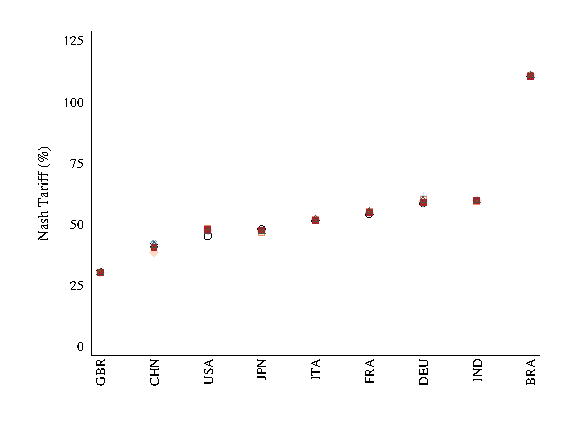
\includegraphics[scale=1.15]{Fig_6}
\par\end{centering}
\noindent\begin{minipage}[t]{1\columnwidth}%
\emph{\footnotesize{}Note:}{\footnotesize{} Each dot corresponds to
the Nash tariff applied on an individual export partner. The tariff-imposing
countries reported on the x-axis are the largest countries in the
2014 WIOD sample, excluding EU members.}%
\end{minipage}
\end{figure}
Next, I compare the welfare losses implied by the baseline approach
to those implied by the approximation-free approach. The comparison
is displayed in Figure \ref{fig: standard method loss}. Once again
it is clear that the two approaches deliver indistinguishable predictions.
Albeit, with different degrees of computational efficiency: on my
personal computer, for instance, the baseline approach produced output
more than 100-times faster than the approximation-free approach, which
itself converged more than 15-times faster than standard optimization-based
approach.

\begin{figure}[!tbh]
\caption{\label{fig: standard method loss}\% Loss in real GDP from a tariff
war}

\centering{}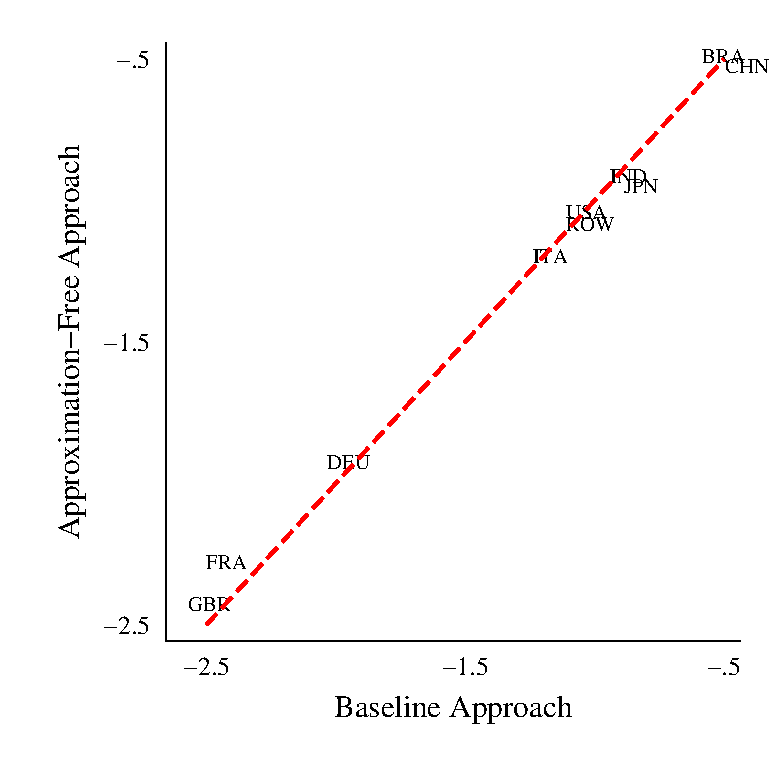
\includegraphics[scale=0.75]{Fig_7}
\end{figure}
Before concluding this appendix, let me reflect more on the computational
speed of the sufficient statistics methodology relative to the standard
iterative method. On the same computing device, my proposed methodology
reduces computation time from multiple hours or even days to \emph{a
few seconds}. Moreover, based on my experience, when smaller countries
are included in the analysis, the standard methodology (based on the
\noun{fmincon} solver in \noun{Matlab}) becomes increasingly sensitive
to the choice of initial values. My purposed methodology, however,
is not susceptible to this problem as it does not involve a numerical
optimization and also imposes \emph{theory-driven} uniformity constraints
on Nash tariffs. Finally, another word caution is that when I implemented
the standard methodology using the \noun{fmincon} solver in \noun{Matlab,
}I obtained output that did not actually correspond to a global optimum
in some instances. I noticed this by cross-checking the output from
\noun{fmincon} with that implied by my analytic formulas and comparing
the objective function's values. This is not a criticism of the standard
iterative methodology per-se, but more so a word caution regarding
the use of \emph{the}\noun{ fmincon} solver. 

\section{List of Industries in Quantitative Analysis}

Table \ref{tab: CP estimation} reports the list of industries in
the quantitative analysis performed in Section \ref{sec:Application}.
To elaborate on this list, the WIOD reports trade and production data
across 56 industries, of which 34 are service-related. To estimate
the industry-level trade elasticities, I group the WIOD industries
into 16 industrial categories. For each industrial category, the trade
elasticity is estimated using the \citet{caliendo2014estimates} methodology,
with specific details provided in Online Appendix G. Unfortunately,
for the ``Mining'' and ``Metal'' industries, my adoption of \citet{caliendo2014estimates}
does not render meaningful estimates for the trade elasticity. Presumably,
this is due to the main exporters in these two industries being WTO
members in 2014, which leads to a lack of sufficient variation in
discriminatory tariffs. As such, I assign \citeauthor{caliendo2014estimates}'s
\citeyearpar{caliendo2014estimates} estimated value to these two
industries. I normalize the trade elasticity in service-related industries
to $\epsilon=4$, following the convention in \citet{costinot2014trade}.
My quantitative results are, however, not sensitive to this normalization
choice, as there is little-to-no foreign trade in service-related
industries.

\begin{table}[tbph]
\caption{\label{tab: CP estimation}List of industries and estimated trade
elasticities.}

\begin{adjustwidth}{-0.25in}{0in}
\begin{center}
\resizebox*{!}{1\textwidth}{
{\renewcommand{\arraystretch}{1.2}
\begin{tabular}{|c|c|c|c|c|} 
										\hline  
\textbf{Number} & \textbf{Description} & \specialcell{trade elasticity \\ $\epsilon_{k}$ } & \specialcell{std. err.} & \specialcell{$N$}  \\ 
										\toprule  
		\multirow{3}{*}{1}& Crop and animal production, hunting & \multirow{3}{*}{0.69} & \multirow{3}{*}{0.12} & \multirow{3}{*}{11,440}\\
		   & Forestry and logging & & & \\
		   & Fishing and aquaculture & & & \\
\hline  2 & Mining and Quarrying & 13.53 & 3.67 & ... \\
\hline  3 & Food, Beverages and Tobacco & 0.47 & 0.13 & 11,440\\
\hline  4 &  Textiles, Wearing Apparel and Leather & 3.33 & 0.53 & 11,480\\
\hline  5 & Wood and Products of Wood and Cork & 5.73 & 0.93 & 11,326 \\
\hline  \multirow{2}{*}{6} & Paper and Paper Products & \multirow{2}{*}{8.50} & \multirow{2}{*}{1.52} & \multirow{2}{*}{11,440}\\
			& Printing and Reproduction of Recorded Media & & &\\
\hline  7 & Coke, Refined Petroleum and Nuclear Fuel & 14.94 & 2.05 & 8,798\\
\hline  \multirow{2}{*}{8} & Chemicals and Chemical Products & \multirow{2}{*}{0.92} & \multirow{2}{*}{0.96} & \multirow{2}{*}{11,440}\\
		  &  Basic Pharmaceutical Products & & & \\
\hline  9 & Rubber and Plastics & 1.69 & 0.78 & 11,480 \\
\hline  10 & Other Non-Metallic Mineral & 1.47 & 0.89 & 11,440 \\
\hline  \multirow{2}{*}{11} & Basic Metals & \multirow{2}{*}{3.28} & \multirow{2}{*}{1.23} & \multirow{2}{*}{...}\\
		   & Fabricated Metal Products & & & \\
\hline  \multirow{2}{*}{12} & Computer, Electronic and Optical Products & \multirow{2}{*}{3.44} & \multirow{2}{*}{1.07} & \multirow{2}{*}{11,480} \\
				& Electrical Equipment & & &\\
\hline  13 & Machinery and Equipment n.e.c & 3.64 & 1.45 & 11,480 \\
\hline  \multirow{2}{*}{14} & Motor Vehicles, Trailers and Semi-Trailers & \multirow{2}{*}{1.38} & \multirow{2}{*}{0.46} & \multirow{2}{*}{11,480}\\
			& Other Transport Equipment & & & \\
\hline  15 & Furniture; other Manufacturing & 1.64 & 0.60 & 11,480 \\
\hline  \multirow{2}{*}{16} & All Service-Related Industries   &  \multirow{2}{*}{4} & \multirow{2}{*}{...} & \multirow{2}{*}{...}  \\
				& (WIOD Industry No. 23-56) & & & \\
   	
							\bottomrule 
\end{tabular} } }
\end{center}
\end{adjustwidth}
\end{table}

\end{document}
